\chapter{Livello di rete}
Il livello di rete nello stack TCP/IP è responsabile della consegna dei datagrammi tra gli host. Questo procedimento comprende numerosi aspetti, come ad esempio la progettazione degli indirizzi logici necessari per identificare in maniera univoca gli host connessi ad Internet. Inoltre, richiede anche degli opportuni protocolli di instradamento che permettano ai pacchetti del livello di rete di giungere dalla sorgente fino alla destinazione.

\section{Introduzione}
\begin{Example}{Comunicazione a livello rete}{}
    \textit{La Figura mostra la comunicazione tra Gaia e Gabriele a livello di rete.}

    \begin{wrapfigure}{r}{0.45\textwidth}
        \vspace{-0.5cm}
        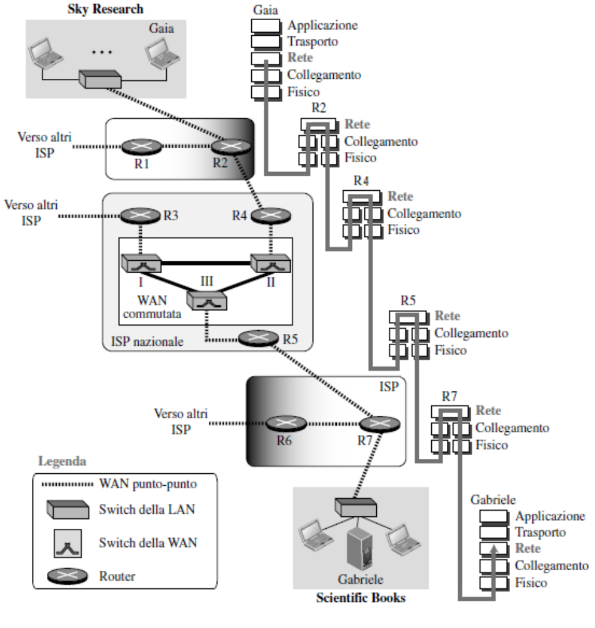
\includegraphics[width=0.45\textwidth]{images/liv-rete.PNG}
        \vspace{-0.5cm}
    \end{wrapfigure}
    
    Come viene mostrato, il livello di rete è presente nell'host sorgente, nell'host destinazione e in tutti i router lungo il percorso (R2, R4, R5 e R7). Nell'host sorgente (Gaia), il livello di rete accetta un pacchetto (più precisamente un segmento o un datagramma utente) dal livello trasporto, incapsula il pacchetto in un datagramma del livello di rete e lo consegna al livello di collegamento. Nell'host di destinazione (Gabriele), il datagramma viene decapsulato, il pacchetto viene estratto e consegnato al livello trasporto. Sebbene gli host sorgente e destinazione siano coinvolti in tutti e cinque i livelli della pila di protocolli TCP/IP, i router utilizzano solamente tre livelli durante l'attività vera e propria di instradamento dei pacchetti. Tuttavia, come vedremo in seguito, i router possono aver bisogno dei livelli di trasporto ed applicazione per alcuni scopi particolari (ad esempio per coordinarsi con altri router). Un router presente lungo il percorso tra sorgente e destinazione normalmente viene rappresentato con almeno due livelli di collegamento e due livelli fisici, in quanto riceve un pacchetto da una rete e lo invia su un'altra rete.    
\end{Example}

\subsection{Servizi a livello rete}
Il ruolo principale del livello di rete è quindi piuttosto semplice: trasferire pacchetti da un host a un altro. \textit{Ma quando un router riceve un pacchetto come fa a sapere a chi deve inviarlo?}

\subsubsection{Instradamento (routing)}
Un compito del livello di rete è l'instradamento (routing). Il compito del livello di rete è quello di instradare il pacchetto dalla sua sorgente alla destinazione. Una rete fisica non è altro che la combinazione di varie altre reti (LAN e WAN) e dei router che le collegano. Ciò significa che, normalmente, c'è più di un percorso che va dalla sorgente alla destinazione. Il livello di rete deve trovare il migliore tra tali possibili percorsi. La scelta del percorso migliore deve avvenire per mezzo di opportune strategie (algoritmi di routing). Nella Internet di oggi questo avviene tramite l'esecuzione di alcuni protocolli di routing (protocolli di instradamento), che hanno lo scopo di aiutare i router a condividere e coordinare la loro conoscenza sulla rete. Il risultato è la creazione di tabelle di instradamento che verranno utilizzate per decidere come instradare i pacchetti al momento del loro arrivo nei router.

\subsubsection{Inoltro (forwarding)}
Se routing significa applicare strategie ed eseguire protocolli per creare tabelle di instradamento in ogni router, l'inoltro (forwarding) si può definire come l'azione eseguita dai router quando un pacchetto arriva ad una delle sue interfacce e lo deve trasferire sull'appropriato collegamento di uscita. La tabella d'inoltro (forwarding table) che viene normalmente utilizzata da un router per completare tale azione viene talvolta definita, in modo piuttosto ambiguo, routing table. Quando un router riceve un pacchetto da una delle reti a cui è collegato direttamente, deve inoltrare il pacchetto ad un'altra delle reti a cui è collegato (nell'instradamento unicast) o a più reti a cui è collegato (nel caso di instradamento multicast). Per prendere questa decisione il router utilizza alcune informazioni che si trovano nell'intestazione del pacchetto, ovvero l'indirizzo di destinazione o un'etichetta, per trovare la giusta interfaccia di output all'interno della tabella d'inoltro.

%\begin{figure}[ht]
%    \centering
%    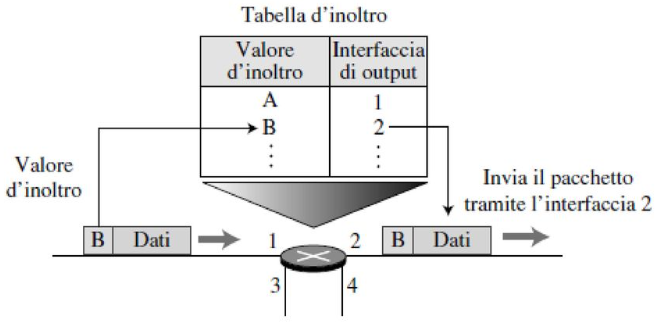
\includegraphics[width=8cm]{images/processo-inoltro.PNG}
%    \caption{Processo d'inoltro}
%    \label{fig:processo-inoltro}
%\end{figure}

\begin{Example}{Tabella di inoltro}{}
    \textit{Il pacchetto con valore del campo di intestazione pari a 0110 giunge a un router che, tramite la propria tabella di inoltro, individua che l'interfaccia in uscita è la 2 a cui lo inoltra internamente.}

    \begin{minipage}{\textwidth}
        \centering
        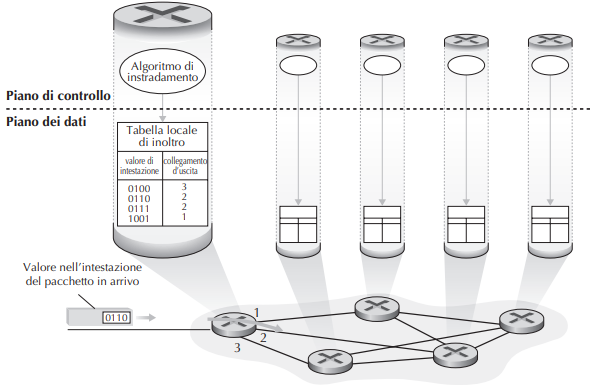
\includegraphics[width=0.7\textwidth]{images/es-tabella-inoltro.PNG}
        %\captionof{figure}{Esempio}
    \end{minipage}
\end{Example}

\subsection{Packet switching}
Dalla discussione su instradamento e inoltro deduciamo che a livello di rete avviene una qualche forma di switching (spostamento). Riserveremo il termine commutatore di pacchetto (packet switch o semplicemente switch) per indicare un generico dispositivo che si occupa del trasferimento dei pacchetti da un'interfaccia in ingresso a quella in uscita, in base al valore dei campi nell'intestazione del pacchetto. Alcuni commutatori di pacchetti, chiamati commutatori a livello di collegamento (link-layer switch), stabiliscono l'inoltro in relazione al valore del campo del frame a livello di collegamento (livello 2). Altri, chiamati router, prendono le decisioni di inoltro basandosi sul valore nel campo a livello di rete (livello 3). Un router infatti è un commutatore di rete che crea un collegamento tra una porta di input e una di output (o un insieme di porte di output).

\begin{Example}{Host, router e commutatori a livello di collegamento}{}
    \textit{La figura mostra il percorso seguito dai dati scendendo lungo la pila di protocolli del sistema mittente, risalendo e scendendo lungo le pile di protocolli dei commutatori e dei router che intervengono a livello di collegamento e, infine, risalendo la pila nel sistema ricevente.}

    \begin{minipage}{\textwidth}
        \centering
        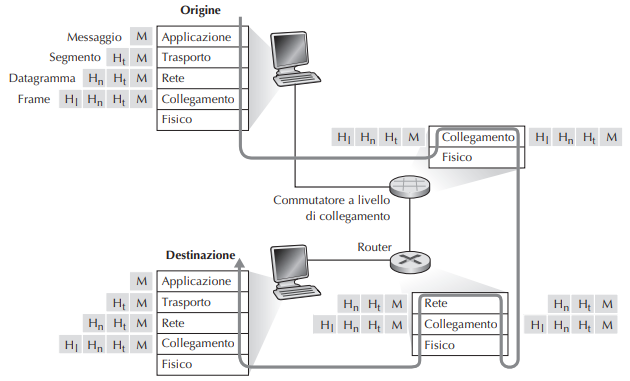
\includegraphics[width=0.7\textwidth]{images/host-router-commutatori.PNG}
        %\captionof{figure}{Esempio}
    \end{minipage}
    
    I router e i commutatori a livello di collegamento sono tutti commutatori di pacchetto. Al pari dei sistemi periferici, organizzano il proprio hardware e software di rete a livelli. In ogni caso non implementano tutti i livelli della pila di protocolli, ma solo quelli inferiori. I commutatori a livello di collegamento implementano i livelli 1 e 2, mentre i router implementano i livelli da 1 a 3. Ciò significa, per esempio, che i router Internet sono in grado di interpretare il protocollo IP (che è di livello 3), mentre i commutatori a livello di collegamento non possono farlo.
\end{Example}

Anche se nella comunicazione dei dati le tecniche di switching sono divise in due ampie categorie, il circuit switching (commutazione di circuito) e il packet switching (commutazione di pacchetto), solo quest'ultimo viene utilizzato a livello di rete in quanto l'unità dei dati, a questo livello, è il pacchetto, mentre il circuit switching viene usato soprattutto al livello fisico. A livello di rete un pacchetto proveniente dal livello superiore (un segmento o un datagramma utente) viene diviso in pacchetti (detti anche datagrammi) di dimensione gestibile ed ognuno di questi viene inviato tramite la rete. La sorgente invia i datagrammi uno alla volta: la destinazione li riceve uno per uno. Visto che durante il percorso è possibile che i datagrammi vengano frammentati in datagrammi più piccoli, la destinazione attende di aver ricevuto tutti i frammenti che fanno parte dello stesso datagramma prima di consegnare il contenuto al livello superiore. I dispositivi di interconnessione, in una rete basata su commutazione di pacchetto, dovranno anche determinare come instradare i datagrammi dalla sorgente alla destinazione finale. Oggi una rete basata su packet switching può utilizzare due approcci diversi per lo switching: l'approccio a datagramma e l'approccio a circuito virtuale.

\subsubsection{Approccio a datagramma: servizio senza connessione}
Con l'obiettivo della semplicità, Internet è stata progettata con un livello di rete in grado di fornire un servizio senza connessione, dove il protocollo di rete tratta ogni datagramma in modo del tutto indipendente ed i singoli datagrammi non hanno alcuna relazione con gli altri. L'idea alla base di questa progettazione è che il livello di rete deve essere solamente in grado di veicolare i datagrammi dalla sorgente alla destinazione. Secondo questo approccio i datagrammi che formano un messaggio (di livello applicazione) possono viaggiare tutti lungo lo stesso percorso verso la destinazione oppure no. Quando il livello di rete fornisce un servizio senza connessione, ogni datagramma che viaggia in Internet è un'entità indipendente, non c'è alcuna relazione tra i datagrammi che appartengono allo stesso messaggio. I commutatori in questo tipo di rete sono normalmente chiamati router.

\begin{figure}[ht]
    \centering
    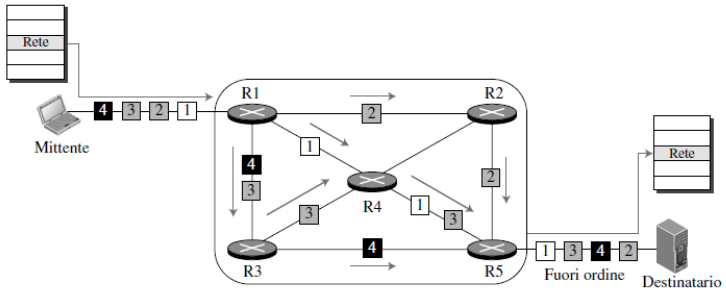
\includegraphics[width=11cm]{images/datagramma-senza-connessione.PNG}
    \caption{Una rete basata su packet switching senza connessione}
    \label{fig:datagramma-senza-connessione}
\end{figure}

Ogni datagramma viene instradato sulla base delle sole informazioni contenute nella sua intestazione: gli indirizzi sorgente e destinazione. L'indirizzo destinazione definisce dove il datagramma deve andare, l'indirizzo sorgente da dove viene. Il router in questo caso instrada il datagramma solo sulla base dell'indirizzo di destinazione. L'indirizzo sorgente può essere utilizzato per inviare un messaggio d'errore alla sorgente nel caso il datagramma venga scartato.

\begin{figure}[ht]
    \centering
    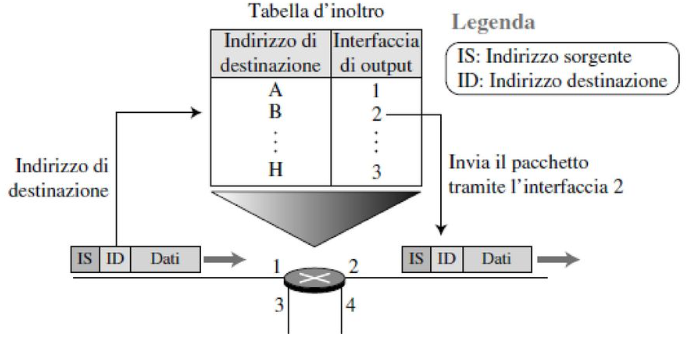
\includegraphics[width=9cm]{images/processo-datagramma-senza-connessione.PNG}
    \caption{Processo d'inoltro di un router in una rete priva di connessione}
    \label{fig:processo-datagramma-senza-connessione}
\end{figure}

\subsubsection{Approccio a circuiti virtuali: servizio orientato alla connessione}
In un servizio orientato alla connessione (chiamato anche approccio a circuiti virtuali) c'è una relazione tra tutti i datagrammi che appartengono a un messaggio (di livello applicazione). Prima che tutti i datagrammi di un messaggio possano essere inviati, è necessario impostare una connessione virtuale per definire il percorso dei datagrammi. Dopo aver impostato la connessione, i datagrammi seguono tutti lo stesso percorso. In questo tipo di servizio, non solo il datagramma deve contenere gli indirizzi sorgente e destinazione, ma deve anche contenere un'etichetta di flusso (flow label), che identifichi il circuito virtuale che definisce il percorso virtuale che il datagramma deve seguire. Anche se può apparire che l'uso dell'etichetta renda inutili gli indirizzi sorgente e destinazione durante la fase di trasferimento dati, bene ricordare che nel caso di Internet il livello di rete continua ad utilizzare tali indirizzi.
Una ragione di questa scelta è che parte del percorso del datagramma può dover utilizzare un servizio senza connessione dove gli indirizzi di sorgente e destinazione rimangono essenziali.

\begin{figure}[ht]
    \centering
    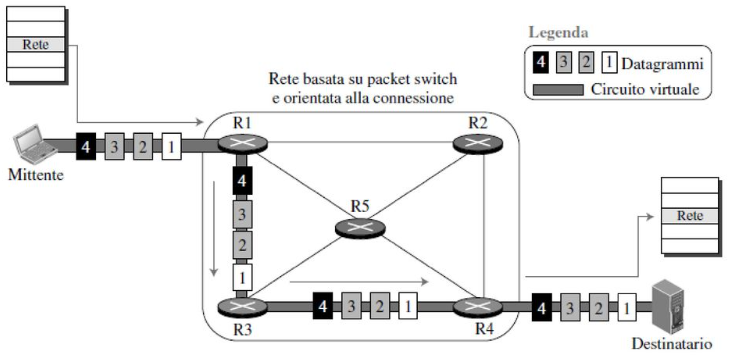
\includegraphics[width=10cm]{images/circuiti-virtuali.PNG}
    \caption{rete basata su circuiti virtuali}
    \label{fig:circuiti-virtuali}
\end{figure}

Ogni datagramma viene inoltrato sulla base dell'etichetta presente nella sua intestazione. Per procedere nel nostro esempio di Internet che utilizza un livello di rete basato su connessione supponiamo che il datagramma abbia già un'etichetta quando raggiunge il router. In questo caso la decisione d'inoltro si basa sul valore dell'etichetta, detta spesso virtual circuit identifier (identificatore del circuito virtuale).

\begin{figure}[ht]
    \centering
    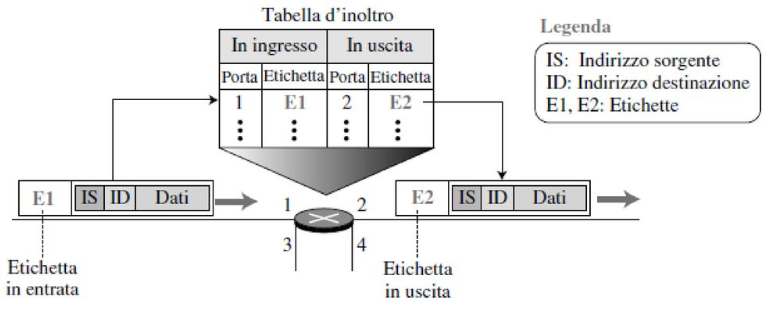
\includegraphics[width=9cm]{images/inoltro-circuito-virtuale.PNG}
    \caption{Inoltro di un router in una rete a circuito virtuale}
    \label{fig:inoltro-circuito-virtuale}
\end{figure}

Per implementare un servizio orientato alla connessione viene utilizzato un processo composto da tre fasi: setup (creazione del circuito virtuale), data transfer (trasferimento dei dati) e teardown (distruzione del circuito virtuale). Nella fase di setup gli indirizzi sorgente e destinazione del mittente e del ricevente vengono utilizzati per configurare nei router le tabelle necessarie per l'impostazione dei circuiti virtuali. Nella fase di teardown la sorgente e la destinazione informano i router di cancellare tutte le informazioni relative al circuito che si sta eliminando. Il trasferimento dei dati avviene necessariamente tra queste due fasi.

\subsection{Struttura di un router}
Nella nostra discussione circa l'inoltro e l'instradamento abbiamo rappresentato il router come una scatola nera che accetta pacchetti in entrata da una delle porte di input (interfacce), usa una tabella d'inoltro per trovare la porta di output e da questa invia il pacchetto. La nostra attenzione sarà specificamente rivolta alla funzione di inoltro: ossia, alle architetture dei router per trasferire i pacchetti dai collegamenti in ingresso a quelli in uscita. 

\subsubsection{Componenti}
Possiamo individuare quattro componenti principali: porte di input, porte di output, processore di routing e switching fabric.

\begin{figure}[ht]
    \centering
    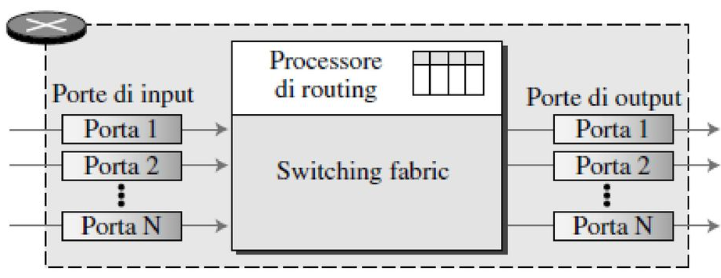
\includegraphics[width=8cm]{images/componenti-router.PNG}
    \caption{Componenti di un router}
    \label{fig:componenti-router}
\end{figure}

\subsubsection{Porte di input}
Una porta di input implementa le funzionalità del livello fisico e di collegamento del router. I bit vengono ricostruiti a partire dal segnale ricevuto. Il datagramma viene estratto dal frame che lo ha trasportato a livello collegamento, viene controllata la presenza di errori e viene quindi scartato se risulta danneggiato. Se il datagramma risulta integro, è pronto per essere processato dal livello di rete. In aggiunta a un processore del livello fisico e un processore del livello di collegamento, la porta di input ha dei buffer (ovvero delle code) per memorizzare i pacchetti in attesa di essere veicolati alla switching fabric.

\begin{figure}[ht]
    \centering
    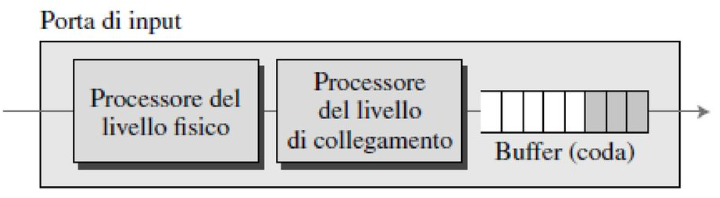
\includegraphics[width=8cm]{images/porta-input-router.PNG}
    \caption{Porta di input di un router}
    \label{fig:porta-input-router}
\end{figure}

\subsubsection{Porte di output}
Una porta di output svolge le stesse funzioni di quella di input, ma in ordine inverso. Per prima cosa i datagrammi in uscita vengono accodati, poi ogni datagramma viene incapsulato in un frame e alla fine per mezzo del livello fisico viene tradotto in un segnale da trasmettere.

\begin{figure}[ht]
    \centering
    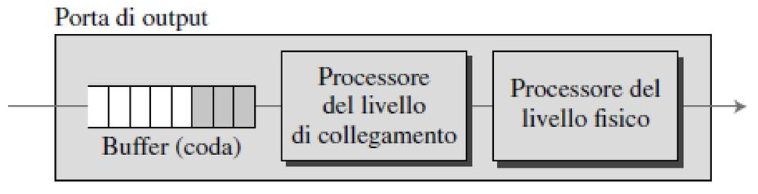
\includegraphics[width=8cm]{images/porta-output-router.PNG}
    \caption{Porta di input di un router}
    \label{fig:porta-output-router}
\end{figure}

\subsubsection{Processore di routing}
Il processore di routing implementa le funzionalità del livello di rete. L'indirizzo di destinazione viene usato per trovare l'indirizzo del salto (hop) successivo, cioè il prossimo apparato a cui inviare il pacchetto e il numero della porta di output da cui il datagramma deve essere spedito. A volte ci si riferisce a tale attività come "ricerca nella tabella" (table lookup) in quanto il processore di routing effettua una ricerca nella tabella d'inoltro. Nei router più recenti, questa funzione del processore di routing viene implementata nelle porte di input per semplificare e rendere più veloce il processo.

\subsubsection{Switching fabric}
Il compito più difficile all'interno di un router è spostare i datagrammi dalla coda di input a quella di output. La velocità con cui ciò viene fatto influisce sulla dimensione delle coda di input/output e sul ritardo complessivo nella consegna del datagramma. In passato, quando un router non era nulla più di un computer dedicato a questo scopo, la memoria del computer, o un bus, venivano usati come infrastruttura interna di comunicazione (la cosiddetta switching fabric). In pratica, la porta di input memorizzava il pacchetto nella memoria del calcolatore e quella di output invece prendeva il pacchetto dalla memoria. Oggi i router usano una varietà di switching fabric progettate per questo specifico scopo.

\subsection{Elaborazione alle porte di ingresso e inoltro}
\begin{figure}[ht]
    \centering
    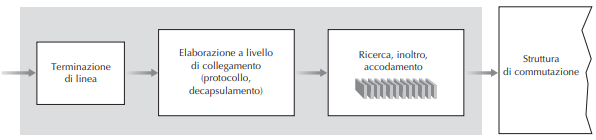
\includegraphics[width=10cm]{images/elaborazione-porte-ingresso.PNG}
    \caption{Elaborazione alle porte di ingresso}
    \label{fig:elaborazione-porte-ingresso}
\end{figure}

Come già detto, la funzione di terminazione della linea e l'elaborazione a livello di collegamento implementano rispettivamente il livello fisico e di collegamento associati a un singolo collegamento di ingresso al router. L'elaborazione effettuata alla porta di ingresso è centrale per la funzionalità del router: è qui che, utilizzando le informazioni della tabella di inoltro, viene determinata la porta di uscita a cui dirigere un pacchetto attraverso la struttura di commutazione. La tabella di inoltro viene elaborata e aggiornata dal processore di instradamento o ricevuta da un controller SDN remoto. Una sua copia conforme è di solito memorizzata su ciascuna porta di ingresso. La tabella di inoltro viene copiata sulla line card dal processore di instradamento tramite un bus separato. Essendoci copie locali della tabella di inoltro, la decisione relativa può essere presa dalle porte di ingresso, senza invocare il processore di instradamento centralizzato.

\begin{Example}{Tabella di inoltro}{}
    \textit{Consideriamo il caso “più semplice” in cui l'inoltro è basato sull'indirizzo di destinazione. Supponiamo che tutti gli indirizzi di destinazione siano a 32 bit (dimensione che è la lunghezza dell'indirizzo di destinazione nei datagrammi IPv4). Un'implementazione elementare della tabella di inoltro presenterebbe una riga per ogni possibile indirizzo di destinazione ma, dato che esistono più di 4 miliardi di possibili indirizzi, questa opzione non viene nemmeno presa in considerazione.}
    
    \textit{Supponiamo inoltre che il nostro router abbia quattro collegamenti, numerati da 0 a 3, e che i pacchetti debbano essere inoltrati verso le interfacce di collegamento come segue:}
    
    \begin{center}
        \begin{tabular}{c c c}
            & \textbf{Intervallo degli indirizzi di destinazione} & \textbf{Interfaccia}\\\hline
            da & 11001000 00010111 00010000 00000000 & \multirow{2}{*}{0}\\
            a & 11001000 00010111 00010111 11111111 &\\\hline
            da & 11001000 00010111 00011000 00000000 & \multirow{2}{*}{1}\\
            a & 11001000 00010111 00011000 11111111 &\\\hline
            da & 11001000 00010111 00011001 00000000 & \multirow{2}{*}{2}\\
            a & 11001000 00010111 00011111 11111111 &\\\hline
            & altrimenti & 3
        \end{tabular}
    \end{center}

    Chiaramente, in questo esempio, non è necessario avere 4 miliardi di righe nelle tabelle di inoltro dei router. Potremmo, per esempio, avere la seguente tabella, con appena quattro voci:

    \begin{center}
        \begin{tabular}{c c}
            \textbf{Corrispondenza di prefisso} & \textbf{Interfaccia}\\
            11001000 00010111 00010 & 0\\
            11001000 00010111 00011000 & 1\\
            11001000 00010111 00011 & 2\\
            altrimenti & 3
        \end{tabular}
    \end{center}

    Con questa struttura il router confronta un prefisso dell'indirizzo di destinazione del pacchetto con una riga della tabella; se c'è corrispondenza, il router inoltra il pacchetto al collegamento associato. Per esempio, supponiamo che l'indirizzo di destinazione del pacchetto sia \texttt{11001000 00010111 00010110 10100001}; dato che il prefisso a 21 bit di questo indirizzo rispecchia la prima riga nella tabella, il router inoltra il pacchetto all'interfaccia di collegamento 0. Se un prefisso non corrisponde alle prime tre righe, il router lo inoltra all'interfaccia 3.

    Sebbene tutto questo sembri sufficientemente semplice, in realtà nasconde un accorgimento ingegnoso. Avrete notato che un indirizzo di destinazione può corrispondere a più di una riga. Per esempio, i primi 24 bit dell'indirizzo \texttt{11001000 00010111 00011000 10101010} corrispondono alla seconda riga della tabella e i primi 21 alla terza riga della tabella. Quando si verificano corrispondenze multiple, il router adotta la regola di corrispondenza a prefisso più lungo; in altre parole, viene determinata la corrispondenza più lunga all'interno della tabella e i pacchetti vengono inoltrati all'interfaccia di collegamento associata.
\end{Example}

\subsection{Struttura di commutazione}
La struttura di commutazione (switching fabric) rappresenta il vero e proprio cuore
dei router, attraverso il quale i pacchetti vengono commutati (ossia inoltrati) dalla
porta di ingresso alla porta di uscita. La commutazione può essere ottenuta in vari
modi.

\begin{figure}[ht]
    \centering
    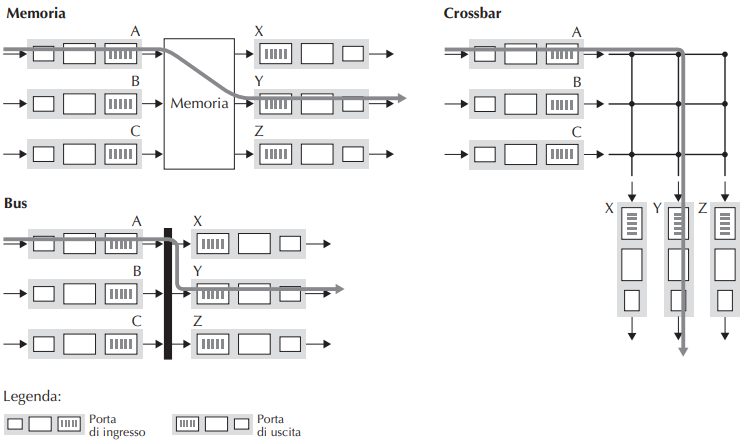
\includegraphics[width=10cm]{images/tecniche-commutazione.PNG}
    \caption{Tre tecniche di commutazione}
    \label{fig:tecniche-commutazione}
\end{figure}

\subsubsection{Commutazione in memoria}
I primi e più semplici router erano in genere calcolatori tradizionali, e la commutazione tra porte di ingresso e di uscita veniva effettuata sotto il controllo diretto della CPU (processore di instradamento). Le porte di ingresso e di uscita funzionavano come tradizionali dispositivi di I/O. Quando sopraggiungeva un pacchetto, la porta di ingresso ne segnalava l'arrivo tramite interrupt e quindi lo copiava nella memoria del processore di instradamento che procedeva a estrarre dall'intestazione l'indirizzo di destinazione. Quindi, individuava tramite la tabella di inoltro l'appropriata porta di uscita nel cui buffer copiava il pacchetto. Notiamo che se l'ampiezza di banda della memoria è tale da potervi scrivere o leggere $B$ pacchetti al secondo, allora il throughput complessivo di inoltro (ossia la velocità massima alla quale i pacchetti vengono trasferiti dalle porte di ingresso a quelle di uscita) è necessariamente inferiore a $B/2$. Notiamo inoltre che due pacchetti non possono essere inoltrati contemporaneamente, anche se hanno differenti porte di destinazione, perché può essere effettuata solo un'operazione alla volta di scrittura/lettura in memoria tramite il bus di sistema.

Anche alcuni router attuali effettuano la commutazione in memoria. Esiste però una differenza sostanziale rispetto ai primi router: la ricerca dell'indirizzo di destinazione e la memorizzazione del pacchetto nella locazione di memoria opportuna vengono effettuate dai processori direttamente sulle line card di ingresso. In alcuni casi, i router che effettuano la commutazione in memoria assomigliano molto a sistemi multiprocessore a memoria condivisa dove l'elaborazione su una line card scrive direttamente i pacchetti nella memoria della porta di uscita appropriata.

\subsubsection{Commutazione tramite bus}
In questo approccio le porte di ingresso trasferiscono un pacchetto direttamente alle porte di uscita tramite un bus condiviso e senza intervento da parte del processore di instradamento. Questo viene tipicamente fatto aggiungendo un'etichetta interna di commutazione (intestazione) al pacchetto che indica la porta locale di output alla quale il pacchetto deve essere trasferito quando viene trasmesso sul bus. Il pacchetto viene ricevuto da tutte le porte di output, ma solo la porta corrispondente all'etichetta lo raccoglierà. L'etichetta viene quindi rimossa dalla porta di output in quanto usata solo all'interno della struttura di commutazione per attraversare il bus. Se più pacchetti arrivano contemporaneamente al router, ognuno su una porta di input diversa, tutti tranne uno dovranno aspettare, dato che sul bus si può trasferire soltanto un pacchetto alla volta. Poiché ciascun pacchetto deve attraversare il bus, la larghezza di banda della commutazione è limitata da quella del bus. Questo tipo di commutazione tramite bus è comunque spesso sufficiente per router che operano in reti di accesso e in quelle aziendali.

\subsubsection{Commutazione attraverso rete di interconnessione}
Un modo per superare la limitazione di banda di un singolo bus condiviso è l'utilizzo di una rete di interconnessione più sofisticata, quale quella usata in passato nelle architetture multiprocessore. Una matrice di commutazione (crossbar switch) è una rete di interconnessione che consiste di $2n$ bus che collegano $n$ porte di ingresso a $n$ porte di uscita. Ogni bus verticale interseca tutti i bus orizzontali a un punto di incrocio che può essere in qualsiasi momento aperto o chiuso dal controller della struttura di commutazione (la cui logica è parte stessa della struttura). Quando un pacchetto giunge a una porta di ingresso A e deve essere inoltrato alla porta Y, il controller chiude l'incrocio di A e Y e la porta A invia il pacchetto sul suo bus e solo il bus Y lo riceverà. Si noti che un pacchetto dalla porta B può essere inoltrato a X nello stesso tempo, perché i pacchetti A-Y e B-X usano bus di input e output diversi. Quindi, al contrario degli altri due approcci, la commutazione attraverso rete di interconnessione è in grado di inoltrare più pacchetti in parallelo. Una matrice di commutazione è non-blocking: un pacchetto in via di inoltro verso una porta di uscita non viene bloccato a meno che esista un altro pacchetto in via di inoltro sulla stessa porta di uscita. Tuttavia, se due pacchetti provenienti da due diverse porte di input sono destinati alla stessa porta di output, uno dovrà accodarsi alla porta di input, perché solo un pacchetto alla volta può essere inoltrato su uno specifico bus.

\subsection{Elaborazione alle porte di uscita}
L'elaborazione alle porte di uscita prende i pacchetti dalla memoria della porta di uscita e li trasmette sul collegamento di uscita. Questo comprende selezionare e togliere dalla coda i pacchetti per la trasmissione e operare le necessarie funzioni a livello di collegamento e fisico.

\begin{figure}[ht]
    \centering
    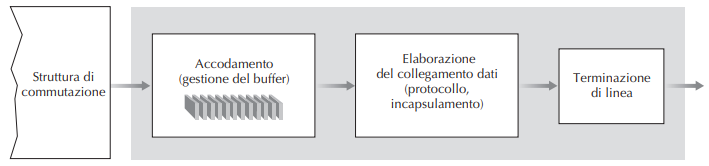
\includegraphics[width=10cm]{images/elaborazione-porte-uscita.PNG}
    \caption{Elaborazione alle porte di uscita}
    \label{fig:elaborazione-porte-uscita}
\end{figure}

\subsection{Dove si verifica l'accodamento?}
E' evidente che si possono formare code di pacchetti sia presso le porte di ingresso sia presso quelle di uscita. Il luogo e la lunghezza della coda (sia alle porte di input che di output) dipendono dalla quantità di traffico di rete, dalle velocità relative della struttura di commutazione e dalla linea. Quando queste code crescono, la memoria del router può esaurirsi e quindi può avvenire una perdita di pacchetti nel caso non vi sia memoria per immagazzinare quelli in arrivo.

\subsubsection{Accodamento in ingresso}
Ma che cosa avviene se la struttura di commutazione non è sufficientemente rapida (rispetto alle linee in ingresso) nel trasferire tutti i pacchetti in arrivo senza ritardo? In questo caso può verificarsi accodamento anche alle porte di ingresso. Per illustrare un'importante conseguenza di tale accodamento, consideriamo una struttura di commutazione facente uso di una rete di interconnessione, e supponiamo che (1) le velocità di tutti i collegamenti siano identiche, (2) un pacchetto possa essere trasferito da qualsiasi porta di ingresso a una data porta di uscita nello stesso intervallo di tempo richiesto perché un pacchetto sia ricevuto su un collegamento di ingresso, e (3) che i pacchetti vengano trasferiti da una coda di ingresso alla relativa coda di uscita desiderata con procedura FCFS (first-come-first-served, primo arrivato primo servito). E' possibile trasferire più pacchetti in parallelo quando le relative porte di uscita sono differenti. Tuttavia, se due pacchetti in testa a due code di ingresso sono destinati alla stessa coda di uscita, allora uno dei pacchetti sarà bloccato e dovrà attendere: istante per istante, la struttura di commutazione può trasferire solo un pacchetto a una certa porta di uscita.

\begin{Example}{HOL: Head Of the Line blocking}{}
    \textit{La figura mostra un esempio in cui due pacchetti (contraddistinti in grigio scuro) in testa alle rispettive code di ingresso sono destinati alla stessa porta di uscita, in alto a destra.} 
    
    \begin{minipage}{\textwidth}
        \centering
        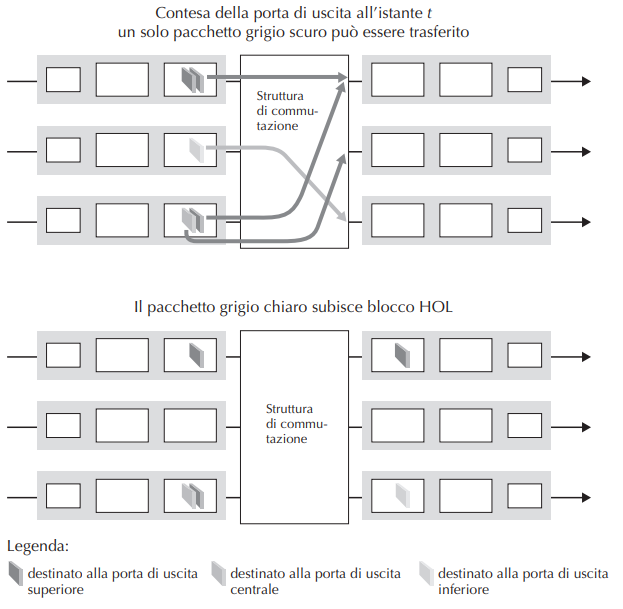
\includegraphics[width=0.7\textwidth]{images/hol.PNG}
        %\captionof{figure}{Esempio}
    \end{minipage}
    
    Supponiamo che la struttura di commutazione scelga di trasferire il primo pacchetto della coda in alto a sinistra. In questo caso, il pacchetto nella coda in basso a sinistra deve attendere, così come quello grigio più chiaro, che si trova dietro di lui, anche se non si verifica contesa per la porta di uscita centrale (che rappresenta la destinazione del pacchetto di colore chiaro). Questo fenomeno è noto come blocco in testa alla coda (HOL, head-of-the-line blocking): un pacchetto nella coda di ingresso deve attendere il trasferimento attraverso la struttura (anche se la propria porta di destinazione è libera) in quanto risulta bloccato da un altro pacchetto che lo precede.
\end{Example}

\subsubsection{Accodamento in uscita}
Dato che la porta di uscita può trasmettere un solo pacchetto in un intervallo prestabilito (tempo di trasmissione del pacchetto), gli $N$ pacchetti in arrivo dovranno mettersi in coda per la trasmissione sul collegamento in uscita. Di conseguenza, è possibile che giungano altri $N$ pacchetti nel periodo necessario per trasmettere solo uno degli $N$ pacchetti già accodati, e così via. Quindi è possibile che si formino code di pacchetti alle porte di uscita e il numero di pacchetti in coda può continuare a crescere fino a esaurire lo spazio di memoria sulla porta di uscita.

In assenza di sufficiente memoria per inserire nel buffer il nuovo pacchetto in ingresso, occorrerà stabilire se scartarlo (politica nota come drop-tail, eliminazione in coda) o se rimuoverne uno o più, fra quelli già in coda, per far posto al nuovo arrivato. In alcuni casi può risultare vantaggioso eliminare un pacchetto (o marcarne l'intestazione) prima che il buffer sia pieno, al fine di fornire al mittente un segnale di congestione.

\begin{Example}{Accodamento alla porta di uscita}{}
    \textit{All'istante $t$, a ciascuna delle porte di ingresso giunge un pacchetto destinato alla porta in uscita superiore. I tre pacchetti originali sono stati trasferiti sulla porta in uscita e sono accodati in attesa di trasmissione.}

    \begin{minipage}{\textwidth}
        \centering
        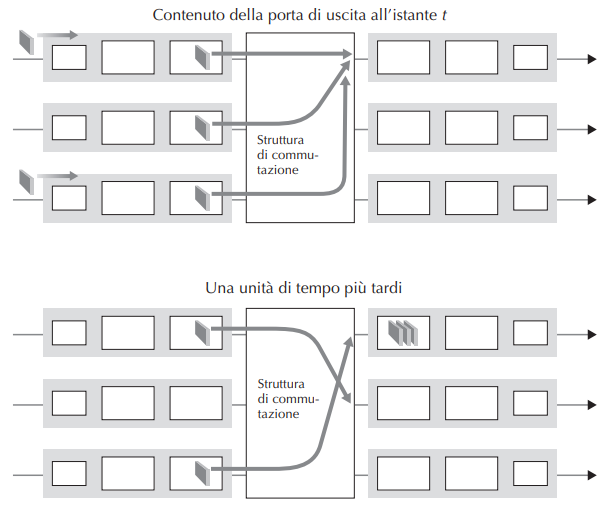
\includegraphics[width=0.7\textwidth]{images/accodamento-porte-uscita.PNG}
        %\captionof{figure}{Esempio}
    \end{minipage}

    Nell'unità di tempo successiva verrà trasmesso uno di questi tre pacchetti. Nel nostro esempio, due nuovi pacchetti sono giunti al commutatore; uno di questi pacchetti è destinato alla porta di uscita superiore. Quando vi sono più pacchetti accodati sulle porte di uscita, uno schedulatore di pacchetti (packet scheduler) deve stabilire in quale ordine trasmetterli. 
\end{Example}

\subsubsection{Capacità dei buffer}
Dato che i buffer nei router sono necessari per assorbire le fluttuazioni del traffico, sorge la domanda su quanto debba essere la loro capacità. Per molti anni la regola empirica usata per dimensionare i buffer era che la quantità di memoria riservata al buffer ($B$) dovesse essere uguale a un RTT medio (per esempio $250 ms$) per la capacità del collegamento ($C$). Questo risultato si basa sull'analisi delle dinamiche di accodamento di un numero relativamente piccolo di flussi TCP. Quindi, un collegamento a $10 Gbps$ con un RTT di $250 ms$ avrebbe bisogno di un buffer pari a $B = RTT * C = 2,5 Gbit$. Recenti studi teorici e sperimentali, tuttavia, suggeriscono che quando c'è un gran numero di flussi TCP ($N$) che passano attraverso un collegamento, la quantità di buffer necessaria sia $B = \frac{RTT*C}{\sqrt{N}}$. Con un gran numero di flussi, che tipicamente attraversano i grossi collegamenti dei router di dorsale, il valore di $N$ può essere grande e la diminuzione nella quantità di buffer necessaria diventa abbastanza significativa.

\section{Protocolli di livello rete}
Nel corso del tempo i protocolli di livello rete hanno avuto molte versioni differenti.

Nella versione 4 il livello di rete può essere visto come formato da un protocollo principale e da tre protocolli ausiliari. Il protocollo principale, l'Internet Protocol versione 4 (IPv4) è responsabile della suddivisione in pacchetti, dell'inoltro (forwarding) e della consegna (delivery) dei datagrammi a livello di rete. L'Internet Control Message Protocol versione 4 (ICMPv4) aiuta l'IPv4 a gestire alcuni errori che possono avvenire nella consegna a livello di rete. L'Internet Group Management Protocol (IGMP) viene utilizzato per supportare l'IPv4 nella gestione del multicasting. Infine, l'Address Resolution Protocol (ARP) viene usato per far interagire il livello di rete e quello di collegamento. Più in dettaglio, ARP ha il compito specifico di permettere l'associazione tra indirizzi di livello di rete ed indirizzi di livello di collegamento.

\begin{figure}[ht]
    \centering
    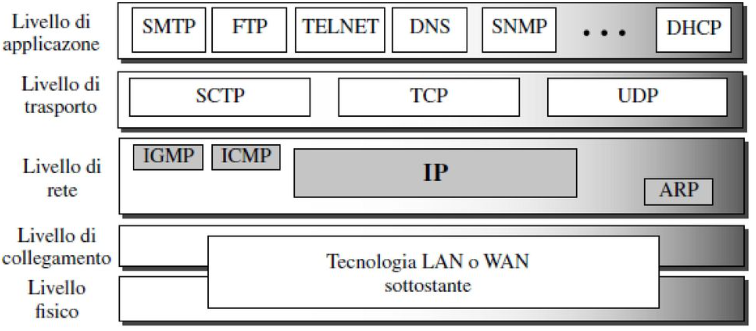
\includegraphics[width=11cm]{images/struttura-logica-tcp-ip.PNG}
    \caption{Struttura logica dello stack TCP/IP}
    \label{fig:struttura-logica-tcp-ip}
\end{figure}

L'IPv4 è un protocollo inaffidabile e senza connessione, basato su datagrammi. IPv4 offre un servizio di consegna di tipo best-effort, ovvero il protocollo fa del suo meglio per consegnare i dati che sono stati spediti ma non offre alcuna garanzia. Con il termine best-effort si intende che i datagrammi IPv4 possono essere danneggiati, persi, arrivare fuori ordine o in ritardo e possono anche generare congestione nella rete. Se è importante l'affidabilità allora è necessario associare ad IPv4 un protocollo di livello trasporto che sia in grado di garantirla aggiungendo alcune funzionalità, come ad esempio il TCP. Un esempio piuttosto semplice di servizio best-effort è l'ufficio postale: fa del suo meglio per consegnare la posta ordinaria ma non sempre ci riesce. Se una lettera non raccomandata viene persa, tocca al mittente (o al potenziale destinatario) scoprire la perdita e risolvere il problema. L'ufficio postale in sé non tiene traccia di ogni lettera e non può notificare al mittente la perdita o il danneggiamento.

\subsection{Formato di datagrammi IPv4}
I pacchetti usati dal protocollo IP vengono definiti datagrammi IP. Un datagramma è un pacchetto di lunghezza variabile composto da due parti: un'intestazione (header) e un campo dati (payload). L'intestazione è lunga da 20 a 60 byte e contiene le informazioni essenziali per il routing e la consegna dei datagrammi. Per comodità di lettura normalmente si rappresenta l'intestazione TCP/IP sotto forma di righe di 4 byte (32 bit) ciascuna.

\begin{figure}[ht]
    \centering
    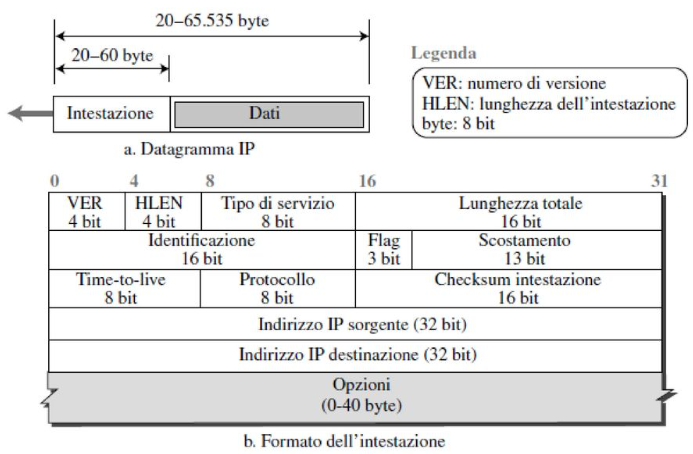
\includegraphics[width=11cm]{images/datagramma-ip.PNG}
    \caption{Datagramma IP}
    \label{fig:datagramma-ip}
\end{figure}

\begin{itemize}
    \item \textit{Numero versione}. Questo campo (VER), formato da 4 bit, definisce la versione del protocollo IP. Visto che si sta trattando IPv4 ovviamente il valore sarà 4.
    \item \textit{Lunghezza dell'intestazione.} Il campo lunghezza intestazione (HLEN), formato da 4 bit. definisce la lunghezza totale dell'intestazione del datagramma in parole formate da 4 byte. Il datagramma IPv4 ha un'intestazione di lunghezza variabile. Quando un dispositivo riceve un datagramma deve sapere dove finisce l'intestazione e dove iniziano i dati incapsulati nel datagramma. La lunghezza dell'intestazione, come numero di byte, deve essere rappresentata facendo uso dei soli 4 bit che formano questo campo. Per questo motivo, si ricorre ad una rappresentazione sotto forma di parole da 4 byte. Questo significa che la lunghezza totale dell'intestazione viene divisa per 4 e il valore inserito nel campo. Il ricevente ovviamente deve moltiplicare il valore di questo campo per 4 per trovare l'effettiva lunghezza totale.
    \item \textit{Tipo servizio.} Secondo la progettazione originaria dell' intestazione IP, questo campo doveva specificare il tipo di servizio (Type Of Service, TOS) ovvero il modo in cui il datagramma doveva essere gestito dai router lungo il percorso. Alla fine degli anni 90, I'IETF ha ridefinito il campo per fornire i cosi detti servizi differenziati (Differentiated Services, DiffServ).
    \item \textit{Lunghezza totale.} Questo campo, da 16 bit, definisce la lunghezza totale (intestazione più dati), espressa in byte, del datagramma IP. Un campo di 16 bit può rappresentare una lunghezza massima di 65.535 byte (nel caso in cui tutti i bit siano impostati a 1). Tuttavia la dimensione dei datagrammi normalmente è molto inferiore a questo massimo. Questo campo è utile al dispositivo ricevente per determinare se il pacchetto in ricezione è arrivato completamente.
    \item \textit{Identificazione, flag e scostamento di frammentazione (offset).} Questi tre campi riguardano la frammentazione dei datagrammi IP che avviene quando la loro dimensione è maggiore rispetto a quella che la tecnologia di livello collegamento sottostante è in grado di trasportare.
    \item \textit{Time-to-live (TTL, tempo di vita).} A causa di alcuni malfunzionamenti dei protocolli di instradamento, può accadere che un datagramma circoli su Internet, visitando alcune reti più di una volta, ma senza raggiungere la destinazione finale. Ovviamente questo porta alla creazione di traffico del tutto inutile. Il campo TTL viene usato per controllare il numero massimo di salti (hop), cioè il numero di router visitati dal datagramma. Quando un host sorgente invia il datagramma, esso memorizza un valore iniziale in questo campo. Questo valore è approssimativamente pari a due volte il numero massimo di salti tra due host qualsiasi presenti su Internet. Ogni router che elabora il datagramma decrementa di una unità questo numero. Se il TTL, dopo essere stato diminuito, giunge a zero allora il router scarta il datagramma.
    \item \textit{Protocollo.} In TCP/IP, la sezione relativa ai dati di un pacchetto, chiamata payload, incapsula l'intero pacchetto di un altro protocollo (solitamente di livello superiore). Un datagramma, per esempio, può portare un pacchetto che appartiene a un protocollo di livello trasporto come UDP (quindi un datagramma utente) o TCP (quindi un segmento). Un datagramma può anche portare un pacchetto di un altro protocollo che usa direttamente il servizio offerto da IP, come ad esempio alcuni protocolli di instradamento o alcuni protocolli ausiliari. Gli enti di gestione Internet hanno assegnato ad ogni protocollo che fa uso del servizio IP un numero univoco composto da 8 bit, numero che viene di volta in volta inserito nel campo protocollo all'interno dell'intestazione. Quando il payload viene incapsulato in un datagramma nella sorgente, il numero di protocollo corrispondente viene inserito in questo campo; quando il datagramma arriva a destinazione, il valore di questo campo permette di definire a quale protocollo va consegnato il payload estratto dal datagramma. In altre parole, questo campo fornisce il multiplexing alla sorgente e il demultiplexing a destinazione.

    \begin{figure}[ht]
        \centering
        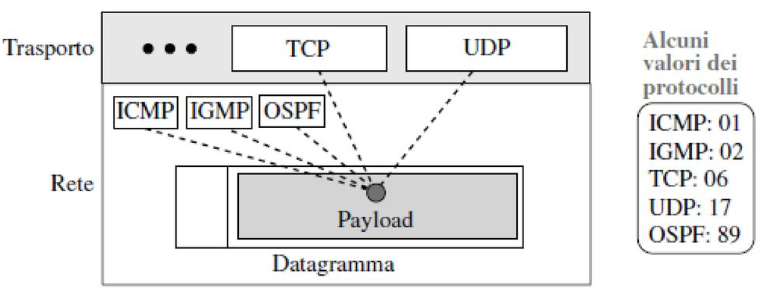
\includegraphics[width=9cm]{images/mult-demult-campo-protocollo.PNG}
        \caption{Multiplexing e demultiplexing utilizzando il valore del campo protocollo}
        \label{fig:mult-demult-campo-protocollo}
    \end{figure}
    
    \item \textit{Checksum dell'intestazione.} IP è un protocollo non affidabile, ad esempio non controlla se i dati incapsulati in un datagramma vengono danneggiati durante la trasmissione. IP lascia l'onere del controllo degli errori nei dati trasmessi al protocollo che è proprietario del payload, come ad esempio UDP o TCP. L'intestazione del datagramma, tuttavia, viene aggiunta dall'IP e il controllo degli errori è quindi di sua responsabilità. Gli errori nell'intestazione IP possono essere un grosso problema. Se l'indirizzo IP di destinazione è danneggiato, il pacchetto sarà consegnato all'host sbagliato. Se il campo protocollo è danneggiato, il payload sarà consegnato al protocollo errato. Se i campi relativi alla frammentazione sono danneggiati, il datagramma non sarà riassemblato correttamente a destinazione, e così via. Per tali ragioni IP aggiunge un campo checksum che riguarda la sola intestazione ma non il payload. E' bene ricordare che, siccome il valore di alcuni campi, come il TTL, la frammentazione e le opzioni, possono cambiare da router a router, il checksum deve essere ricalcolato in ogni router. Il checksum, che viene inserito in un campo da 16 bit, è ottenuto come il complemento della somma degli altri campi dell'intestazione, il tutto utilizzando l'aritmetica complemento a uno.
    \item \textit{Indirizzi sorgente e destinazione.} Questi campi, lunghi 32 bit, definiscono rispettivamente l'indirizzo IP della sorgente e quello della destinazione. L'host sorgente dovrebbe conoscere a priori il suo indirizzo IP. L'indirizzo IP di destinazione è invece noto al protocollo che utilizza il servizio offerto da IP oppure viene ottenuto per mezzo del DNS. Da notare che il valore di questi campi deve rimanere immutato durante tutto il tragitto del datagramma IP dall'host sorgente a quello di destinazione.
    \item \textit{Opzioni.} L'intestazione di un datagramma può avere fino a 40 byte di opzioni. Le opzioni posso essere usate per il test o il debug della rete. Anche se le opzioni non sono una parte necessaria dell'intestazione IP, è richiesto che tutte le implementazioni di IP siano in grado di gestirle, quando presenti.
    \item \textit{Payload (dati).} I dati trasportati ovviamente sono la ragione principale per la creazione del datagramma. Il payload è il pacchetto che deriva dagli altri protocolli che usano il servizio dell'IP, siano questi di livello superiore (per esempio, TCP e UDP) o di pari livello (per esempio, ICMP) nello stack TCP/IP. Equiparando un datagramma ad un pacchetto postale, il payload è il contenuto del pacchetto, mentre l'intestazione è solo l'informazione scritta sul pacco.
\end{itemize}

\subsection{Frammentazione}
Per giungere alla destinazione, un datagramma IP può dover viaggiare attraverso varie reti, ognuna con caratteristiche differenti. Ogni router toglie il datagramma dal frame di livello collegamento che ha ricevuto, lo elabora e poi lo incapsula in un nuovo frame. Il formato e la dimensione del frame ricevuto dipendono dalla tecnologia fisica e da quella di livello di collegamento utilizzati per trasportare il frame. Viceversa, il formato e le dimensione del frame inviato dipendono dalla tecnologia fisica e da quella di livello di collegamento della rete su cui il frame verrà inviato. Per esempio se un router collega una LAN ad una WAN, riceverà un frame in formato LAN e invierà un nuovo frame in formato WAN.

\subsubsection{Maximum Transfer Unit (MTU)}
Ogni protocollo di livello collegamento ha il proprio formato di frame. Una delle caratteristiche di ciascun formato è la dimensione massima del payload che può essere incapsulato nel frame. In altre parole, quando un datagramma è racchiuso in un frame, la dimensione totale del datagramma deve essere inferiore rispetto a questa misura massima, che è definita dalle restrizioni imposte dall'hardware e dal software usati nella rete. Il valore dell'MTU differisce tra i diversi protocolli di livello collegamento e fisico. Per esempio il valore per una LAN normalmente è di 1.500 byte, ma per una WAN può essere maggiore o inferiore.

\begin{figure}[ht]
    \centering
    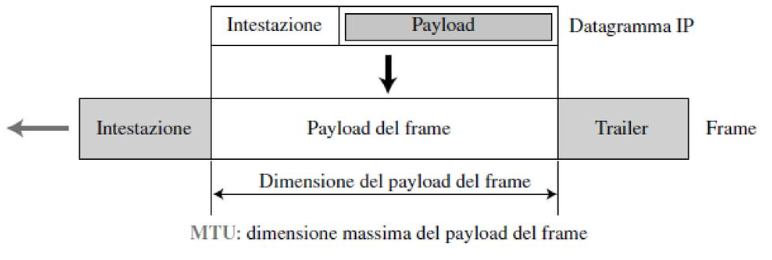
\includegraphics[width=9cm]{images/mtu.PNG}
    \caption{Matximux Transfer Unit (MTU)}
    \label{fig:mtu}
\end{figure}

Per rendere il protocollo IP indipendente dai livelli sottostanti, i progettisti hanno deciso di fissare la lunghezza massima del datagramma IP a 65.535 byte. Questo rende la trasmissione efficiente nel caso si usi un protocollo di livello collegamento con una MTU di tali dimensioni. Tuttavia, altre tecnologie di rete richiedono che il datagramma sia suddiviso in parti più piccole per poter essere trasportato. Questo procedimento viene chiamato frammentazione.

Quando un datagramma IP viene frammentato ogni frammento ha la propria intestazione, nella maggior parte dei casi i campi dell'intestazione sono uguali rispetto al datagramma originario ma alcuni devono essere cambiati. Un datagramma frammentato può essere a sua volta frammentato se incontra una rete con una MTU ancora più piccola. In altre parole un datagramma può essere frammentato più volte prima di raggiungere la sua destinazione finale.

Un datagramma può essere frammentato dall'host sorgente o da qualsiasi altro router lungo il percorso verso la destinazione. Il riassemblaggio del datagramma, tuttavia, viene fatto solo dall'host di destinazione, in quanto ogni frammento diventa un datagramma indipendente.

I diversi frammenti del datagramma originario possono viaggiare lungo percorsi differenti: questi percorsi non sono prevedibili o controllabili a priori ma, alla fine, tutti i frammenti che appartengono allo stesso datagramma dovrebbero arrivare all'host destinazione. Quindi è logico che il riassemblaggio avvenga solamente alla destinazione finale. Oltretutto, il riassemblaggio dei pacchetti durante il percorso provocherebbe una significativa perdita di efficienza.

Quando parliamo di frammentazione non intendiamo solamente che il payload del datagramma IP viene frammentato. Infatti, la maggior parte dell'intestazione, ad eccezione di alcune opzioni, deve essere copiata nell'intestazione di tutti i frammenti. L'host o il router che frammenta un datagramma IP deve cambiare i valori di tre campi dell'intestazione: i flag, lo scostamento di frammentazione e la lunghezza totale. Il resto dei campi dell'intestazione deve invece essere solamente copiato. Naturalmente il valore del checksum va ricalcolato ad ogni hop indipendentemente dalla frammentazione.

\subsubsection{Campi relativi alla frammentazione}
Abbiamo detto in precedenza che tre campi nell'intestazione del datagramma IP si riferiscono alla frammentazione: identificazione, flag e scostamento di frammentazione (offset).
\begin{itemize}
    \item Il campo identificazione, da 16 bit, identifica un datagramma che ha origine da un host sorgente. La combinazione tra indirizzo IP sorgente e campo identificazione deve definire in modo unico un datagramma quando lascia l'host sorgente. Per garantire l'unicità, il protocollo IP utilizza un contatore per etichettare i datagrammi. Il contatore viene inizializzato a un numero positivo. Quando il protocollo IP invia un datagramma, copia il valore corrente del contatore nel campo identificazione ed incrementa il contatore di uno. Quando un datagramma viene frammentato il valore nel campo identificazione viene copiato in tutti i frammenti ottenuti. In altre parole tutti i frammenti hanno lo stesso numero di identificazione, che è anche lo stesso del datagramma originale. Il numero d'identificazione aiuta la destinazione a riassemblare il datagramma. Esso sa che tutti i frammenti con lo stesso valore d'identificazione vanno assemblati in un unico datagramma IP.
    \item Il campo flag, da 3 bit, in realtà definisce tre flag distinti, ognuno composto da un singolo bit. Il bit all'estrema sinistra è riservato (non viene attualmente usato). Il secondo bit (bit D) è definito do not fragment (non frammentare). Se il suo valore è 1 allora il dispositivo non deve frammentare il datagramma. Se non è in grado di trasmettere il datagramma attraverso nessuna delle reti fisiche allora lo scarta ed invia un messaggio d'errore ICMP all'host sorgente. Se il suo valore è 0, se necessario, il datagramma può essere frammentato. Il terzo bit (bit M) detto more fragments, nel caso sia impostato a 1 indica che questo datagramma non è l'ultimo frammento della serie e che ci sono altri frammenti dopo di lui. In altre parole non si tratta dell'ultimo frammento di un datagramma originario. Se il suo valore è 0 significa che è l'ultimo (o l'unico) frammento.
    \item Il campo scostamento di frammentazione (offset), da 13 bit, mostra la posizione relativa di questo frammento rispetto all'intero datagramma. E' l'offset dei dati nel datagramma originario misurato in unità da 8 byte.

    \begin{Example}{Frammentazione: offset}{}
        \textit{La Figura mostra il payload di datagramma con una dimensione di 4000 byte suddiviso in tre frammenti.} 
        
        \begin{minipage}{\textwidth}
            \centering
            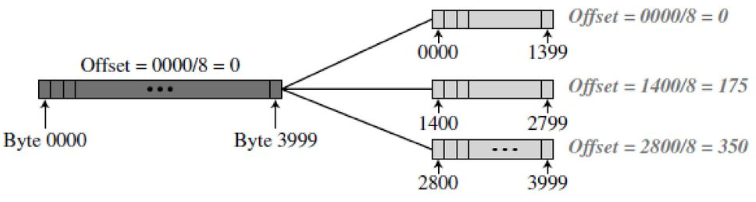
\includegraphics[width=0.7\textwidth]{images/es-frammentazione.PNG}
            %\captionof{figure}{Esempio}
        \end{minipage}
        
        I dati nel datagramma originario sono numerati da 0 a 3999. Il primo frammento porta i byte da 0 a 1399. L'offset per questo datagramma è 0/8 = 0. Il secondo frammento porta i byte da 1400 a 2799, il valore offset per questo frammento è 1400/8 = 175. Infine il terzo frammento porta i byte da 2800 a 3999. Il valore offset per questo frammento è 2800/8 = 350.
    \end{Example}

    E' necessario ricordare che il valore dell'offset viene misurato in unità da 8 byte. Questo avviene perché la lunghezza del campo offset è di soli 13 bit e non può rappresentare una sequenza di byte maggiore di 8191. Ciò costringe gli host o i router che frammentano i datagrammi a scegliere la dimensione dei frammenti in modo che sia divisibile per 8, ad esclusione ovviamente dell'ultimo frammento originato dalla suddivisione di un datagramma.
\end{itemize}

\begin{Example}{Frammentazione}{}
    \textit{La figura mostra una visione espansa dei frammenti dell'esempio precedente.} 
    
    \begin{minipage}{\textwidth}
        \centering
        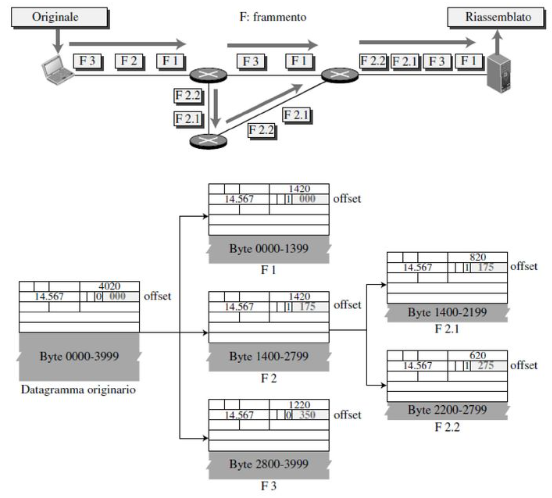
\includegraphics[width=0.6\textwidth]{images/es-frammentazione2.PNG}
        %\captionof{figure}{Esempio}
    \end{minipage}
    
    Il pacchetto originario viene generato da un host client, i frammenti vengono riassemblati nel server. Il valore del campo identificazione è lo stesso in tutti i frammenti, e il valore del flag more fragments è impostato a 1 in tutti i frammenti ad esclusione dell'ultimo. Inoltre nella figura viene mostrato il valore del campo offset per ogni frammento. Da notare che anche se i frammenti sono arrivati fuori ordine alla destinazione, possono essere riassemblati correttamente.
    
    La figura mostra inoltre cosa avviene se un frammento viene anch'esso frammentato. In questo caso il valore del campo offset si riferisce sempre al datagramma originario. Per esempio nella figura il secondo frammento è a sua volta frammentato in due frammenti da 800 e da 600 byte, ma l'offset mostra la posizione relativa dei frammenti rispetto ai dati originali. E' ovvio che anche se ogni frammento segue un percorso differente ed arriva in disordine, l'host di destinazione finale può riassemblare il datagramma originario dai frammenti ricevuti (se nessuno di essi è andato perso), utilizzando la seguente strategia:
    \begin{enumerate}
        \item Il primo frammento ha un valore del campo offset pari a 0.
        \item Dividere per 8 la lunghezza del primo frammento. Il secondo frammento ha un valore offset pari a tale risultato.
        \item Dividere per 8 la somma della lunghezza del primo e del secondo frammento. Il terzo frammento ha un valore offset pari a tale risultato.
        \item Continuare il procedimento. L'ultimo frammento ha il suo bit M impostato a 0.    
    \end{enumerate}
\end{Example}

\subsection{Indirizzi IPv4}
Generalmente un host ha un solo collegamento con la rete; quando l'implementazione di IP dell'host vuole inviare un datagramma, lo fa su tale collegamento. Il confine tra host e collegamento fisico viene detto interfaccia. Invece, dato che il compito di un router è ricevere datagrammi da un collegamento e inoltrarli su un altro, questo deve necessariamente essere connesso ad almeno due collegamenti. Anche il confine tra un router e i suoi collegamenti è chiamato interfaccia. Il router presenta più interfacce, una su ciascuno dei suoi collegamenti. Dato che host e router sono in grado di inviare e ricevere datagrammi, IP richiede che tutte le interfacce abbiano un proprio indirizzo IP. Pertanto, l'indirizzo IP è tecnicamente associato a un'interfaccia, anziché all'host o al router che la contiene.

Gli indirizzi IP sono lunghi 32 bit (4 byte). Tali indirizzi sono solitamente scritti nella cosiddetta notazione decimale puntata (dotted-decimal notation), in cui ciascun byte dell'indirizzo viene indicato in forma decimale ed è separato con un punto dagli altri byte dell'indirizzo. Ogni interfaccia di host e router di Internet ha un indirizzo IP globalmente univoco. Una parte dell'indirizzo di un'interfaccia è determinata dalla sottorete cui è collegata.

\begin{Example}{Indirizzi delle interfacce e sottoreti}{}
    \textit{La figura mostra un router (con tre interfacce) che connette sette host.} 
    
    \begin{minipage}{\textwidth}
        \centering
        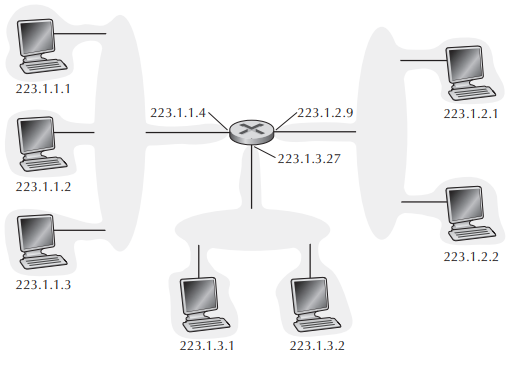
\includegraphics[width=0.6\textwidth]{images/es-sottoreti.PNG}
        %\captionof{figure}{Esempio}
    \end{minipage}
    
    I tre a sinistra e l'interfaccia del router cui sono connessi hanno un indirizzo IP della forma \texttt{233.1.1.xxx}: ossia, i 24 bit più a sinistra nell'indirizzo IP sono identici. Le quattro interfacce sono interconnesse da una rete che non contiene router. Per adesso rappresentiamo la rete priva di router che connette questi host come una nuvola. 

    Per IP, questa rete che interconnette tre interfacce di host e l'interfaccia di un router forma una sottorete. IP assegna a questa sottorete l'indirizzo \texttt{223.1.1.0/24}, dove la notazione \texttt{/24}, detta anche maschera di sottorete (subnet mask), indica che i 24 bit più a sinistra dell'indirizzo definiscono l'indirizzo della sottorete. Di conseguenza, la sottorete \texttt{223.1.1.0/24} consiste di tre interfacce di host (\texttt{223.1.1.1}, \texttt{223.1.1.2}, \texttt{223.1.1.3}) e di un'interfaccia di router (\texttt{223.1.1.4}). Ogni altro host connesso alla sottorete \texttt{223.1.1.0/24} deve avere un indirizzo della forma \texttt{223.1.1.xxx}.
\end{Example}

\subsubsection{Spazio degli indirizzi (address space)}
Un protocollo come l'IPv4 che utilizza degli indirizzi ha bisogno di definire uno spazio di indirizzi, cioè il numero totale di indirizzi utilizzati dal protocollo. Se un protocollo usa $b$ bit per rappresentare un indirizzo, lo spazio degli indirizzi è pari a $2^b$ perché ogni bit può assumere solo due valori distinti (0 o 1). IPv4 usa indirizzi a 32 bit, il che significa che lo spazio degli indirizzi è $2^{32}$ o 4.294.967.296 (più di quattro miliardi). Se non ci fosse alcuna restrizione, oltre 4 miliardi di dispositivi potrebbero essere collegati a Internet.

Esistono tre notazioni comunemente usate per rappresentare gli indirizzi IPv4: la notazione binaria (base 2), la notazione decimale puntata (base 256) e quella esadecimale (base 16). Nella notazione binaria un indirizzo IPv4 viene rappresentato con 32 bit. Per facilitare la lettura dell'indirizzo normalmente vengono inseriti uno o più spazi tra ogni ottetto (8 bit). Spesso ci si riferisce a ciascun ottetto come ad un byte. Per rendere l'indirizzo IPv4 più compatto e facile da leggere normalmente viene scritto in forma decimale, con un punto che separa i byte. Questo formato viene definito notazione decimale puntata (dotted-decimal notation). Da notare che siccome ogni byte (ottetto) è formato da soli 8 bit, ogni numero nella notazione decimale puntata è compreso tra 0 e 255. A volte è possibile trovare un indirizzo IPv4 espresso in notazione esadecimale. In questo caso ogni cifra esadecimale equivale a quattro bit. Ciò significa che un indirizzo a 32 bit ha 8 cifre esadecimali. Tale notazione viene spesso utilizzata nella programmazione di rete.

\begin{figure}[ht]
    \centering
    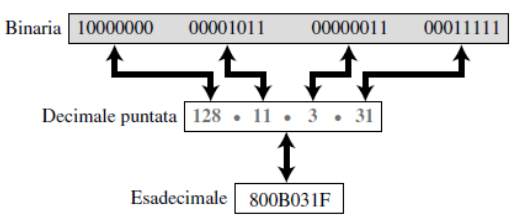
\includegraphics[width=9cm]{images/notazioni-indirizzi.PNG}
    \caption{Tre diverse notazioni per l'indirizzamento IPv4}
    \label{fig:notazioni-indirizzi}
\end{figure}

In ogni rete di comunicazione in cui è prevista la consegna di un messaggio da un mittente ad un destinatario il meccanismo di indirizzamento è gerarchico. Anche gli indirizzi IPv4 sono gerarchici, ma divisi in sole due parti. La prima parte dell'indirizzo, chiamata prefisso (prefix), identifica la rete, mentre la seconda parte dell'indirizzo, chiamata suffisso (suffix), identifica il nodo nella rete (o meglio il collegamento di un dispositivo a Internet).

\begin{figure}[ht]
    \centering
    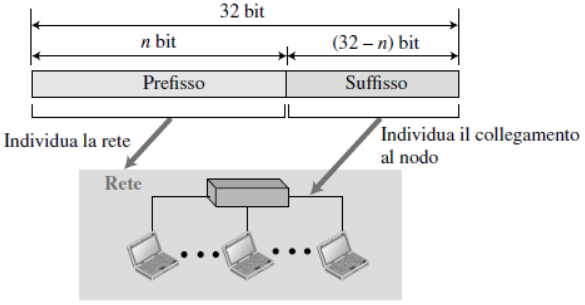
\includegraphics[width=9cm]{images/gerarchia-indirizzamento.PNG}
    \caption{Gerarchia dell'indirizzamento}
    \label{fig:gerarchia-indirizzamento}
\end{figure}

Un prefisso può avere una lunghezza fissa o variabile. Il sistema di identificazione delle reti in IPv4 è stato inizialmente progettato come prefisso a lunghezza fissa. Questo schema, che ormai è obsoleto, viene indicato come indirizzamento con classi (classful addressing). Il nuovo schema, chiamato indirizzamento senza classi (classless addressing), usa un prefisso di rete di lunghezza variabile.

\subsubsection{Indirizzamento con classi}
Come detto in precedenza, inizialmente l'indirizzamento IPv4 era stato progettato con un prefisso di lunghezza fissa, ma vista la necessità di supportare sia reti piccole che grandi, al posto di una sola lunghezza di prefisso ne erano state previste tre ($n = 8$ , $n = 16$ e $n = 24$). L'intero spazio degli indirizzi era stato diviso in cinque classi (classe A, B, C, D ed E).

\begin{figure}[ht]
    \centering
    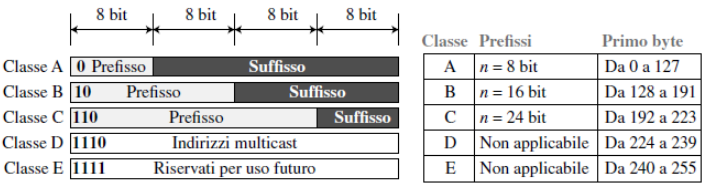
\includegraphics[width=11cm]{images/indirizzamento-con-classi.PNG}
    \caption{Indirizzamento con classi}
    \label{fig:indirizzamento-con-classi}
\end{figure}

Nella classe A la lunghezza della parte di rete è di 8 bit, ma siccome il primo bit, che è 0, identifica il tipo di classe, possiamo avere solo sette bit per l'identificazione delle reti. Ciò significa che ci sono solo $2 ^ 7 = 128$ reti al mondo che possono avere un indirizzo di classe A. Nella classe B la lunghezza della parte di rete è di 16 bit, ma siccome i primi due bit, che sono (10) 2 identificano la classe, possiamo avere solo 14 bit per identificare reti. Ciò significa che ci sono solo $2 ^{14} = 16.384$ reti al mondo che possono avere un indirizzo di classe B.

Tutti gli indirizzi che iniziano con (110), appartengono alla classe C, nella quale la lunghezza della parte di rete è di 24 bit, ma siccome tre bit definiscono la classe, possiamo avere solo 21 bit per identificare le reti. Ciò significa che ci sono $2 ^{21} = 2.097$ reti al mondo che possono avere un indirizzo di classe C.

Gli indirizzi che iniziano con (1110), appartengono alla classe D. una classe che non è divisa in prefisso e suffisso ed è usata per gli indirizzi di tipo multicast. Infine, la classe E raccoglie tutti gli indirizzi che iniziano con (1111). Come per la classe D, la classe E non è divisa in prefisso e suffisso ed è riservata per uso futuro.

La ragione per cui l'indirizzamento con classi è diventato obsoleto è l'esaurimento degli indirizzi. Siccome gli indirizzi non sono stati assegnati in modo appropriato, Internet ha dovuto affrontare il problema dell'esaurimento degli indirizzi disponibili per società ed individui che volevano collegarsi in rete. Per comprendere meglio il problema pensiamo alla classe A. Tale classe può essere assegnata solo a 128 organizzazioni al mondo, ma a causa della struttura della classe A ognuna deve avere una singola rete con 16.777.216 nodi (computer collocati in questa unica rete). Siccome ci sono ben poche organizzazioni così grandi, la maggior parte degli indirizzi in questa classe è andata sprecata (gran parte degli indirizzi erano assegnati ma rimanevano inutilizzati). Gli indirizzi di classe B sono stati progettati per le organizzazioni di media dimensione, ma anche in questo caso molti degli indirizzi sono rimasti inutilizzati. Gli indirizzi di classe C hanno un difetto di progettazione completamente diverso. Il numero di indirizzi disponibile in ogni rete (256) era talmente piccolo che la maggior parte delle organizzazioni non lo trovavano adeguato per le proprie esigenze. Infine, gli indirizzi di classe E erano riservati per uso futuro, sprecando l'intera classe.

\subsubsection{Indirizzamento senza ciassi}
Con la crescita di Internet era chiaro che, come soluzione a lungo termine, sarebbe servito uno spazio degli indirizzi più grande. Tuttavia, questa soluzione richiede necessariamente che la lunghezza degli indirizzi IP venga aumentata, il che significa anche che il formato dei datagrammi IP deve essere modificato. Anche se la soluzione a lungo termine è già stata ideata ed implementata (si chiama IPv6), è stata studiata anche una soluzione a breve termine. In questa soluzione si continua ad usare lo stesso spazio degli indirizzi ma si cambia la loro distribuzione, attraverso un approccio più equo. La soluzione a breve termine è ancora basata sugli indirizzi IPv4 ma non fa più uso della divisione in classi. In altre parole la suddivisione in classi è stata rimossa per compensare la scarsità di indirizzi disponibili.

Gli enti di gestione di Internet hanno annunciato una nuova struttura chiamata indirizzamento senza classi. In questa forma di indirizzamento vengono utilizzati dei blocchi di lunghezza variabile che non appartengono a nessuna classe. Possiamo avere un blocco da 1, 2, 4, 128 indirizzi e così via.

Il prefisso in un indirizzo definisce il blocco (individua la rete): il suffisso definisce il nodo (individua il dispositivo). In teoria possiamo avere un blocco di $2^0, 2^1, 2^2 ...$ indirizzi. Ad un'organizzazione si può quindi assegnare un blocco di indirizzi di dimensione adeguata alla sue esigenze.

A differenza dell'indirizzamento con classi, la lunghezza del prefisso nell'indirizzamento senza classi è variabile. Possiamo avere una lunghezza di prefisso che va da 0 a 32 bit. La dimensione della parte di rete è inversamente proporzionale alla lunghezza del prefisso. Un prefisso piccolo implica una rete più grande (con molti nodi al suo interno), un prefisso grande implica una rete più piccola (con pochi nodi).

Siccome la lunghezza del prefisso non è più parte integrante dell'indirizzo è necessario aggiungere questa informazione in modo separato. In questo caso la lunghezza del prefisso, $n$, viene aggiunta all'indirizzo separata da una barra (slash). La strategia di assegnazione degli indirizzi Internet è detta classless interdomain routing. CIDR generalizza la nozione di indirizzamento di sottorete. L'indirizzo IP viene diviso in due parti e mantiene la forma decimale puntata $a.b.c.d/x$, dove $x$ indica il numero di bit nella prima parte dell'indirizzo.
Gli $x$ bit più a sinistra di un indirizzo della forma $a.b.c.d/x$ costituiscono la porzione di rete dell'indirizzo IP e sono spesso detti prefisso (di rete) dell'indirizzo.

\begin{figure}[ht]
    \centering
    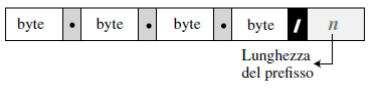
\includegraphics[width=7cm]{images/cidr.PNG}
    \caption{Numerazione slash (CIDR)}
    \label{fig:cidr}
\end{figure}

A un'organizzazione viene generalmente assegnato un blocco di indirizzi contigui con
un prefisso comune per tutti gli indirizzi IP dei dispositivi che si trovano al suo interno. I rimanenti $32-x$ bit di un indirizzo possono essere usati per distinguere i dispositivi interni dell'organizzazione, che hanno tutti lo stesso prefisso di rete.

Dato un indirizzo IP appartenente ad un blocco di indirizzi, normalmente vogliamo ricavare tre informazioni riguardo il suo blocco di appartenenza: il numero di indirizzi che contiene, il primo indirizzo del blocco e l'ultimo. Siccome la lunghezza del prefisso, $n$, è nota, possiamo facilmente ottenere queste tre informazioni.
\begin{enumerate}
    \item Il numero di indirizzi nel blocco è dato da $N = 2^{32-n}$.
    \item Per trovare il primo indirizzo, teniamo invariati i primi $n$ bit partendo da sinistra e impostiamo a 0 tutti i bit restanti a destra (sono $32-n$).
    \item Per trovare l'ultimo indirizzo, teniamo invariati i primi $n$ bit partendo da sinistra e impostiamo a 1 tutti i bit restanti a destra (anche in questo caso sono $32-n$).
\end{enumerate}

\begin{figure}[ht]
    \centering
    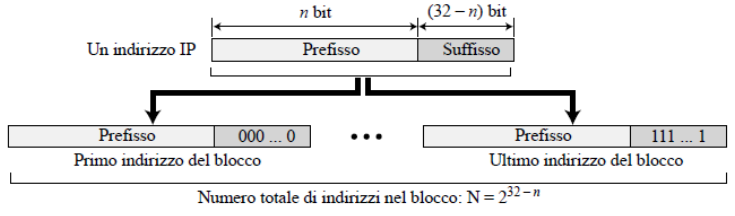
\includegraphics[width=11cm]{images/estrazione-informazioni.PNG}
    \caption{Estrazione delle informazioni nell'indirizzamento senza classi}
    \label{fig:estrazione-informazioni}
\end{figure}

Un altro modo per trovare il primo e l'ultimo indirizzo del blocco è usare la maschera dell'indirizzo (address mask), cioè un numero composto da 32 bit in cui i primi $n$ bit a sinistra sono impostati a 1 e il resto dei bit ($32-n$) sono impostati a 0. Il motivo principale per utilizzare una notazione di questo tipo è che può essere usata da un programma per calcolare in modo efficiente le informazioni di un blocco, usando solamente tre semplici operatori sui bit: NOT, AND e OR.

\begin{enumerate}
    \item Il numero degli indirizzi nel blocco è N = NOT (maschera) + 1.
    \item Il primo indirizzo nel blocco = (qualsiasi indirizzo del blocco) AND (maschera)
    \item L'ultimo indirizzo nel blocco = (qualsiasi indirizzo nel blocco) OR (NOT (maschera)).
\end{enumerate}

\subsubsection{Indirizzo di rete (network address)}
Il primo indirizzo, detto indirizzo di rete (network address), è particolarmente importante in quanto è usato nell'instradamento dei datagrammi verso la rete di destinazione. Per il momento supponiamo che Internet sia composta da $m$ reti e da un router con $m$ interfacce. Quando un datagramma giunge al router da un qualsiasi host sorgente, il router deve sapere a quale rete va inviato il datagramma e quindi da quale interfaccia va inviato. Quando il datagramma arriva alla rete di destinazione, raggiungerà l'host di destinazione utilizzando un'altra strategia. Dopo che il network address è stato trovato, il router consulta la sua tabella d'inoltro per trovare l'interfaccia corrispondente dalla quale inviare il datagramma. L'indirizzo di rete in realtà è lo strumento per l'identificazione delle reti: ogni rete è identificata per mezzo del suo network address.

\begin{figure}[ht]
    \centering
    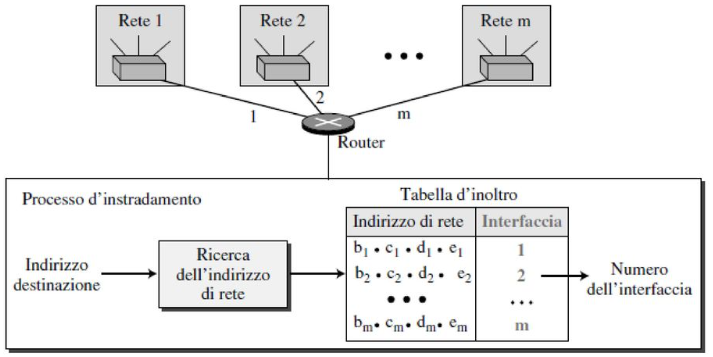
\includegraphics[width=10cm]{images/network-address.PNG}
    \caption{Indirizzo di rete (network address)}
    \label{fig:network-address}
\end{figure}

Prima di terminare l'argomento degli indirizzi IPv4 dobbiamo parlare di cinque indirizzi speciali che vengono usati per scopi particolari: l'indirizzo this-host, l'indirizzo limited-broadcast, l'indirizzo di loopback.
\begin{itemize}
    \item \textit{Indirizzo this-host.} L'unico indirizzo del blocco 0.0.0.0/32 viene chiamato indirizzo this-host (questo host). Viene usato ogni volta che un host ha la necessità di inviare un datagramma IP ma non conosce il proprio indirizzo da usare come indirizzo sorgente.
    \item \textit{Indirizzo limited-broadcast.} L'unico indirizzo nel blocco 255.255.255.255/32 viene chiamato indirizzo limited-broadcast. Viene usato ogni volta che un router o un host devono inviare un datagramma a tutti i dispositivi che si trovano all'interno della rete. I router della rete, bloccano i datagrammi che hanno questo indirizzo come destinazione, in questo modo la sua diffusione sarà limitata alla rete locale.
    \item \textit{Indirizzo di loopback.} Il blocco 127.0.0.0/8 viene chiamato indirizzo di loopback. Un datagramma con uno degli indirizzi in questo blocco come indirizzo di destinazione non lascia mai l'host di spedizione, rimane al suo interno. Questi indirizzi vengono usati per il test e debug del software in esecuzione sull'host locale.
\end{itemize}

\subsubsection{Ottenere indirizzi IP}
Per ottenere un blocco di indirizzi IP da usare in una sottorete, un amministratore di
rete deve innanzitutto contattare il proprio ISP e ottenere un blocco di indirizzi contigui con un prefisso comune. I router esterni alla rete dell'organizzazione considerano solo gli $x$ bit del prefisso, cioè, quando un router all'esterno dell'organizzazione inoltra un datagramma avente un indirizzo di destinazione che è interno, dovrà considerare solo i primi $x$ bit dell'indirizzo. Questo riduce in modo considerevole la dimensione della tabella di inoltro dei router, dato che una sola riga della forma $a.b.c.d/x$ è sufficiente per far pervenire i pacchetti all'organizzazione. I rimanenti $32-x$ bit di un indirizzo possono essere usati per distinguere i dispositivi interni dell'organizzazione, che hanno tutti lo stesso prefisso di rete. Saranno quindi i router della rete interna che utilizzeranno i restanti bit dell'indirizzo per indirizzarli al dispositivo destinatario. Tali bit potrebbero presentare un'aggiuntiva struttura di sottorete.

Rivolgersi a un ISP è solo un modo per ottenere un blocco di indirizzi, ma non è l'unico. Anche perché lo stesso ISP deve richiedere, a sua volta, un blocco di indirizzi. Esiste un'autorità globale che ha la responsabilità ultima di gestire lo spazio di indirizzamento IP e di allocare i blocchi di indirizzi: l'Internet Corporation for Assigned Names and Numbers (ICANN). Il ruolo di ICANN non è solo allocare indirizzi IP, ma anche gestire i root DNS server. Ha anche il compito, assai controverso, di assegnare e risolvere dispute sui nomi di dominio.

\subsubsection{Dynamic Host Configuration Protocol (DHCP)}
Un'organizzazione che ha ottenuto un blocco di indirizzi li può assegnare individualmente alle interfacce di host e router nella propria struttura. Per gli indirizzi delle interfacce dei router, l'amministratore di sistema configura manualmente gli indirizzi IP nel router (spesso da remoto, tramite uno strumento di gestione della rete). Gli indirizzi degli host possono essere configurati manualmente, ma più spesso questo compito è svolto utilizzando il dynamic host configuration protocol (DHCP). DHCP consente a un host di ottenere un indirizzo IP in modo automatico. L'amministratore di rete può configurare DHCP di modo che un dato host riceva un indirizzo IP persistente, in modo che ogni volta che l'host entra in rete gli venga assegnato sempre lo stesso indirizzo IP, oppure in modo da assegnare a ciascun host che si connette un indirizzo IP temporaneo, che sarà diverso tutte le volte che l'host si collega alla rete. 

DHCP viene spesso detto protocollo plug-and-play o zero-conf (zero-configuration) per la sua capacità di automatizzare la connessione degli host alla rete. Questa peculiarità lo rende molto interessante per gli amministratori di rete che, altrimenti, dovrebbero svolgere questi compiti manualmente. DHCP è anche largamente usato nelle reti residenziali di accesso a Internet e nelle LAN wireless, dove gli host arrivano e se ne vanno con estrema frequenza dalla rete.

DHCP è un protocollo client-server. Un client è di solito un host appena connesso che desidera ottenere informazioni sulla configurazione della rete, non soltanto su uno specifico indirizzo IP. Nel caso più semplice, ogni sottorete dispone di un server DHCP. In caso contrario, è necessario un agente di relay DHCP (generalmente implementato in un router), che conosca l'indirizzo di un server DHCP per quella rete.
In aggiunta al suo indirizzo IP, un computer necessita anche di conoscere il proprio prefisso di rete (o la maschera di rete dell'indirizzo). La maggior parte dei computer ha bisogno anche di altre due informazioni: l'indirizzo di un router di default che deve essere usato per comunicare con le altre reti (oltre a quella locale) e l'indirizzo di almeno un server per la risoluzione dei nomi. Riassumendo, normalmente servono quattro informazioni fondamentali: l'indirizzo del computer, il prefisso, l'indirizzo del default router e l'indirizzo IP del server dei nomi di dominio. DHCP può essere usato per fornire tutte queste informazioni all'host.

Per i nuovi host, il protocollo DHCP si articola in quattro punti:
\begin{enumerate}
    \item \textit{Individuazione del server DHCP.} Il primo compito di un host appena collegato è l'identificazione del server DHCP con il quale interagire. Questa operazione è svolta utilizzando un messaggio DHCP discover, che un client invia in un pacchetto UDP attraverso la porta 67. Il pacchetto UDP è incapsulato in un datagramma IP. Ma a chi dovrebbe essere inviato questo datagramma? L'host non conosce ancora l'indirizzo IP della rete alla quale è collegato e ancor meno l'indirizzo di un server DHCP per quella rete. Detto ciò, il client DHCP crea un datagramma IP contenente il suo messaggio DHCP con l'indirizzo IP di destinazione broadcast di 255.255.255.255 e l'indirizzo IP sorgente di 0.0.0.0, cioè “questo host”. Il client DHCP inoltra il datagramma IP al suo livello di collegamento, che invia il frame in broadcast a tutti i nodi collegati alla sottorete.
    \item \textit{Offerta del server DHCP.} Un server DHCP, che riceve un messaggio di identificazione, risponde al client con un messaggio DHCP offer, che viene inviato in broadcast a tutti i nodi della sottorete, usando di nuovo l'indirizzo IP broadcast 255.255.255.255. Dato che in una sottorete possono essere presenti diversi server DHCP, il client dovrebbe trovarsi nell'invidiabile posizione di essere in condizione di scegliere tra le diverse “offerte” disponibili. Ciascun messaggio di offerta server contiene l'ID di transazione del messaggio di identificazione ricevuto, l'indirizzo IP proposto al client, la maschera di sottorete e la durata della concessione (lease time) dell'indirizzo IP (il lasso di tempo durante il quale l'indirizzo IP sarà valido). Tale valore è comunemente dell'ordine delle ore o dei giorni.
    \item \textit{Richiesta DHCP.} Il client appena collegato sceglierà tra le offerte dei server e risponderà con un messaggio DHCP request, che riporta i parametri di configurazione.
    \item \textit{Conferma DHCP.} Il server risponde al messaggio di richiesta DHCP con un messaggio DHCP ACK, che conferma i parametri richiesti.
\end{enumerate}

Il DHCP è un protocollo client/server nel quale il client invia un messaggio di richiesta e il server invia un messaggio di risposta. Nella Figura \ref{fig:messaggi-dhcp} viene mostrato il formato generale dei messaggi DHCP.

\begin{figure}[ht]
    \centering
    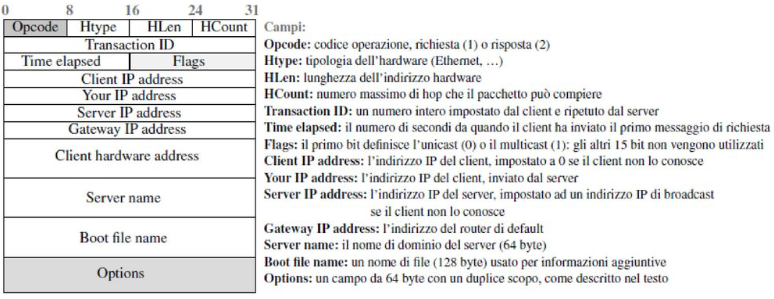
\includegraphics[width=11cm]{images/messaggi-dhcp.PNG}
    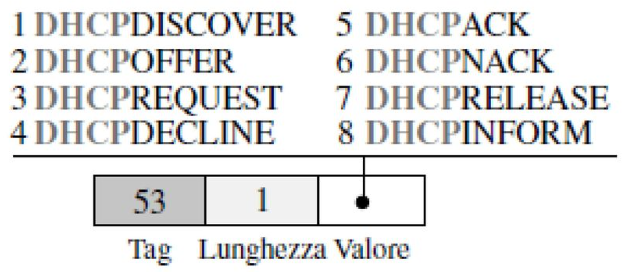
\includegraphics[width=4cm]{images/formato-opzioni.PNG}
    \caption{Formato dei messaggi e delle opzioni DHCP}
    \label{fig:messaggi-dhcp}
\end{figure}

Il campo \verb|Options| (composto da 64 bit) ha un duplice scopo. Può trasportare informazioni aggiuntive oppure la specifica di opzioni DHCP. Per scegliere quest'ultima possibilità, il server utilizza un numero, chiamato magic cookie, sotto forma di un indirizzo IP con valore \texttt{99.130.83.99}, ed inserisce questo valore nei primi 4 byte del campo opzioni del pacchetto di risposta. Quando il cliente legge una risposta cerca il magic cookie nel campo opzioni del pacchetto ricevuto. Se è presente allora i 60 byte successivi sono opzioni. Un'opzione è composta da tre campi: un campo tag da 1 byte, un campo lunghezza da 1 byte e un campo valore di lunghezza variabile. Ci sono numerosi campi tag che vengono usati e possono anche differire a seconda delle implementazioni. Se il campo tag è 53 allora il campo valore definisce uno degli 8 tipi di messaggio illustrati nella Figura \ref{fig:messaggi-dhcp}.

\begin{Example}{Funzionamento del DHCP}{}
    \textit{Viene illustrato un semplice scenario di funzionamento del DHCP.}

    \begin{minipage}{\textwidth}
        \centering
        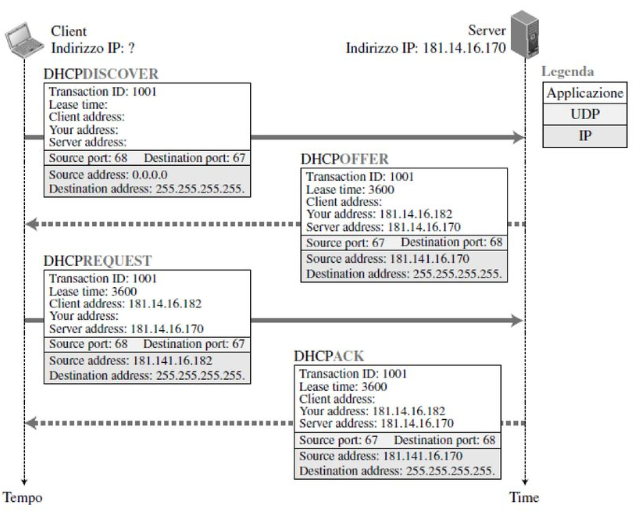
\includegraphics[width=0.7\textwidth]{images/es-dhcp.PNG}
        %\captionof{figure}{Esempio}
    \end{minipage}

    \begin{enumerate}
        \item L'host che vuole entrare in rete crea un messaggio di tipo \texttt{DHCPDISCOVER} nel quale solo il campo \texttt{transaction-ID} viene impostato usando un numero generato casualmente. L'host non può impostare alcun altro campo in quanto non ha le informazioni necessarie per farlo. Questo messaggio viene incapsulato in un datagramma utente UDP con porta sorgente impostata a 68 e la porta destinazione impostata a 67, entrambe sono porte note. Il datagramma utente viene quindi incapsulato in un datagramma IP con indirizzo sorgente impostato a 0.0.0.0 ("this-host") e l'indirizzo di destinazione impostato a 255.255.255.255 (indirizzo broadcast). Il motivo è semplice, l'host al momento non conosce né il proprio indirizzo né quello del server.
        \item Il server o i server DHCP (ce ne possono essere più di uno) rispondono con un messaggio di tipo \texttt{DHCPOFFER} nel quale il campo \texttt{your-IP-address} contiene l'indirizzo IP offerto per l'host che ne ha fatto richiesta e il \texttt{server-IP-address} comprende l'indirizzo IP del server. Il messaggio contiene anche un lease time (tempo di concessione), cioè per quanto tempo l'host potrà far uso di quell'indirizzo IP. Questo messaggio di risposta viene incapsulato in un datagramma utente con gli stessi numeri di porta della richiesta, ma ovviamente in ordine inverso. Il datagramma utente a sua volta viene incapsulato in un datagramma IP con l'indirizzo del server come indirizzo IP sorgente, ma l'indirizzo destinazione è ancora un indirizzo broadcast. Questo è utile anche per consentire agli altri server DHCP di ricevere l'offerta e fornire un'offerta migliore, qualora possano.
        \item L'host richiedente riceve una o più offerte e seleziona la migliore. A questo punto l'host deve inviare un messaggio di tipo \texttt{DHCPREQUEST} al server che ha inviato l'offerta migliore. Tutti i campi con valore noto vengono impostati. Il messaggio viene incapsulato in un datagramma utente con numeri di porta uguali al primo messaggio di richiesta. Il datagramma utente viene incapsulato in un datagramma IP con l'indirizzo sorgente impostato al nuovo indirizzo assegnato al client, ma l'indirizzo di destinazione è ancora impostato all'indirizzo broadcast. Questo è necessario per annunciare a tutti gli altri server che la loro offerta non è stata accettata.
        \item Infine, il server selezionato risponde con un messaggio di tipo \texttt{DHCPACK} al client se l'indirizzo IP offerto è valido. Se il server non è più in grado di mantenere la sua offerta (per esempio se nel frattempo l'indirizzo è stato offerto ad un altro host), il server invia un messaggio di tipo \texttt{DHCPNACK} e il client deve ripetere il procedimento. Anche questo messaggio è broadcast per far sapere agli altri server se la richiesta è stata accettata o rifiutata.
    \end{enumerate}
\end{Example}

\subsubsection{NAT}
La distribuzione degli indirizzi per mezzo degli ISP ha creato un nuovo problema. Supponiamo che un ISP abbia assegnato un blocco di indirizzi di dimensione molto limitata ad una piccola azienda o a una famiglia. Se l'azienda cresce o la famiglia necessita di un blocco più ampio, l'ISP potrebbe non essere in grado di soddisfare la richiesta in quanto gli indirizzi che precedono o seguono il blocco possono essere già stati assegnati ad altre reti.

La proliferazione di sottoreti “small office, home office” (o SOHO, piccoli uffici in ambiente domestico), sembrerebbe implicare che ogni volta che si voglia installarne una, l'ISP debba allocare un intervallo di indirizzi per coprire tutte le macchine della sottorete. Di conseguenza, al crescere della LAN dovrebbe esserle allocato un blocco maggiore di indirizzi. Ma che cosa avverrebbe se l'ISP avesse già allocato la parte contigua all'intervallo di indirizzi dell'attuale rete SOHO? E che cosa dovrebbe sapere il normale utente per gestire gli indirizzi IP? Fortunatamente, esiste un approccio più semplice e sempre più usato: il NAT (network address translation). Questa tecnologia consente di usare una serie di indirizzi privati per la comunicazione interna e una serie di indirizzi Internet globali (almeno uno) per la comunicazione con il resto del mondo. In questo modo, la rete interna necessita di un solo collegamento all'Internet globale, per mezzo di un router in grado di effettuare le operazioni di NAT.

\begin{figure}[ht]
    \centering
    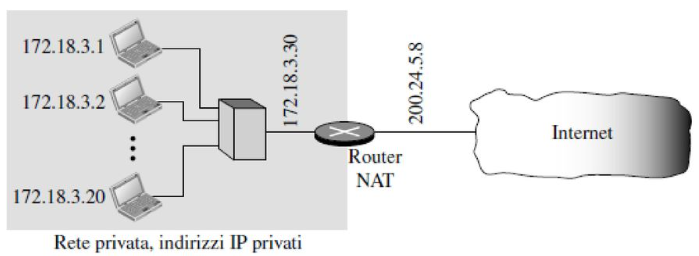
\includegraphics[width=10cm]{images/nat.PNG}
    \caption{Network Address Translation (NAT)}
    \label{fig:nat}
\end{figure}

Come mostrato in Figura \ref{fig:nat}, la rete privata utilizza solamente indirizzi IP privati. Il router che collega la rete interna ad Internet utilizza due indirizzi IP, uno privato e uno globale (pubblico). E' bene notare che la rete privata risulta invisibile al resto di Internet, dall'esterno è possibile rilevare solamente il router NAT con indirizzo pubblico \texttt{200.24.5.8}.

Tutti i pacchetti in uscita dalla rete privata passano tramite il router NAT, che sostituisce l'indirizzo IP sorgente presente nel datagramma con l'indirizzo NAT globale del router (l'indirizzo pubblico). Anche tutti i pacchetti in entrata passano tramite il router NAT, che in questo caso sostituisce l'indirizzo destinazione nel pacchetto (l'indirizzo globale del router NAT) con l'indirizzo privato appropriato (quello dell'host nella rete interna).

Ma se gli indirizzi privati hanno significato solo all'interno di una data rete, come viene gestito l'indirizzamento dei pacchetti relativi all'Internet globale, in cui gli indirizzi sono necessariamente univoci? La risposta è il NAT. I router abilitati al NAT non appaiono come router al mondo esterno, ma si comportano come un unico dispositivo con un unico indirizzo IP.

Contestualmente, ci si potrebbe chiedere dove i calcolatori della rete domestica ottengano i propri indirizzi e dove il router acquisisca il proprio indirizzo IP. Spesso la risposta è DHCP. Il router ottiene il proprio indirizzo dal server DHCP dell'ISP e manda in esecuzione un server DHCP per fornire gli indirizzi ai calcolatori all'interno dello spazio di indirizzamento della rete domestica. Se tutti i datagrammi in arrivo al router NAT dalla rete geografica hanno lo stesso indirizzo IP di destinazione (nello specifico, quello dell'interfaccia sul lato WAN del
router NAT), allora come apprende il router a quale host interno dovrebbe essere inoltrato un determinato datagramma? Il trucco consiste nell'utilizzare una tabella di traduzione NAT (NAT translation table) nel router NAT e nell'includere nelle righe di tale tabella i numeri di porta oltre che gli indirizzi IP.

\begin{Example}{NAT}{}
    \textit{La figura mostra l'attività di un router abilitato al NAT, con un'interfaccia che fa parte della rete domestica (sulla destra della figura).}
    
    \begin{minipage}{\textwidth}
        \centering
        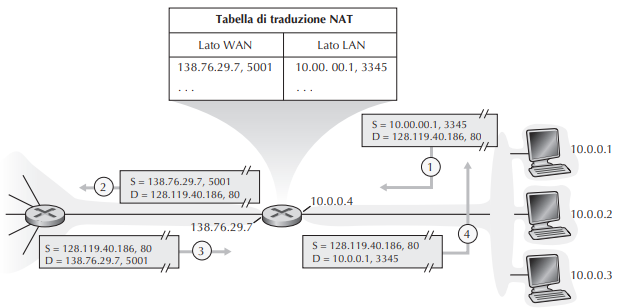
\includegraphics[width=0.7\textwidth]{images/es-nat.PNG}
        %\captionof{figure}{Esempio}
    \end{minipage}
    
    Come visto in precedenza, le quattro interfacce della rete domestica hanno lo stesso indirizzo di sottorete, \texttt{10.0.0.0/24}. Lo spazio di indirizzamento \texttt{10.0.0.0/8} è una delle tre parti dello spazio di indirizzi IP riservato alle reti private, o reame (realm) con indirizzi privati: ossia, una rete i cui indirizzi hanno significato solo per i dispositivi interni. In effetti, esistono centinaia di migliaia di reti private, molte delle quali usano un identico spazio di indirizzamento, \texttt{10.0.0.0/24}, per scambiare pacchetti fra i loro dispositivi. 
    
     Nella figura tutto il traffico che lascia il router domestico verso Internet ha l'indirizzo IP di origine \texttt{138.76.29.7} e tutto il traffico in entrata deve avere lo stesso indirizzo come destinazione. In sostanza, il router abilitato al NAT nasconde i dettagli della rete domestica al mondo esterno.

     Supponiamo che un utente che si trovi nella rete domestica dietro l'host \texttt{10.0.0.1} richieda una pagina web da un server (porta 80) con indirizzo IP \texttt{128.119.40.186}. L'host \texttt{10.0.0.1} assegna il numero di porta di origine (arbitrario) 3345 e invia il datagramma nella rete locale. Il router NAT riceve il datagramma, genera per esso un nuovo numero di porta di origine 5001, sostituisce l'indirizzo IP sorgente con il proprio indirizzo IP sul lato WAN \texttt{138.76.29.7} e sostituisce il numero di porta di origine iniziale 3345 con il nuovo numero 5001. Quando genera un nuovo numero di porta di origine, il router NAT può selezionare qualsiasi numero di porta che attualmente non si trova nella tabella di traduzione NAT. Notiamo che, essendo il campo numero di porta lungo 16 bit, il protocollo NAT può supportare più di 60.000 connessioni simultanee con un solo indirizzo IP sul lato WAN relativo al router. Il NAT del router aggiunge inoltre una riga alla propria tabella di traduzione NAT. Il web server, ignaro della manipolazione subita dal datagramma in arrivo con la richiesta HTTP, risponde con un datagramma con l'indirizzo IP del router NAT come destinazione e il cui numero di porta di destinazione è 5001. Quando questo datagramma arriva al router NAT, quest'ultimo consulta la tabella di traduzione NAT usando l'indirizzo IP di destinazione e il numero di porta di destinazione per ottenere l'appropriato l'indirizzo IP (\texttt{10.0.0.1}) e il corretto numero di porta di destinazione (3345) del browser nella rete domestica. Il router quindi riscrive l'indirizzo di destinazione del datagramma e il suo numero di porta di destinazione e inoltra il datagramma nella rete domestica.
\end{Example}

\subsection{Inoltro dei datagrammi IP}
Come abbiamo detto in precedenza, inoltrare significa collocare il pacchetto nel giusto percorso che lo porterà a destinazione. Dato che oggi Internet è costituita da una combinazione di collegamenti (reti), inoltrare significa inviare il pacchetto al salto (hop) successivo (che può essere la destinazione finale o un dispositivo d'interconnessione intermedio).

\subsubsection{Inoltro basato sull'indirizzo di destinazione}
Per prima cosa ci occuperemo dell'inoltro basato sull'indirizzo di destinazione. Questo è l'approccio tradizionale, e oggi è quello prevalente. Questo approccio richiede che l'host o il router che deve effettuare il forwarding abbia una tabella d'inoltro. Quando un host ha un datagramma da inviare o quando un router ha ricevuto un datagramma da inoltrare, esso fa riferimento a questa tabella per trovare il salto successivo a cui inviare il datagramma.


Il compito del modulo di forwarding è quello di effettuare le ricerche nella tabella. In ciascuna riga, gli $n$ bit a sinistra nell'indirizzo di destinazione (prefisso) sono lasciati invariati e il resto dei bit (suffisso) sono impostati a 0. Se l'indirizzo risultante (chiamato indirizzo di rete) combacia con l'indirizzo nella prima colonna, allora l'informazione nelle successive due colonne viene estratta. In caso contrario la ricerca continua. Normalmente l'ultima riga ha un valore di default nella prima colonna che rappresenta tutti gli indirizzi di destinazione che non combaciano con le righe precedenti (in generale si dice quindi che è una "riga di default").

\begin{Example}{Tabella d'inoltro}{}
    \textit{Realizzare una tablella d'inoltro per il router R1 utilizzando la configurazione mostrata in figura.}

    \begin{minipage}{\textwidth}
        \centering
        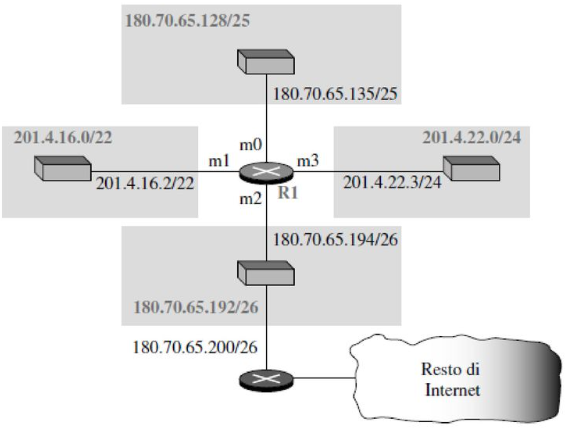
\includegraphics[width=0.5\textwidth]{images/es-tab-inoltro.PNG}
        %\captionof{figure}{Esempio}
    \end{minipage}

    La tabella risultante è la seguente:
    \begin{center}
    \begin{tabular}{|l|l|l|}
         \hline\textit{Indirizzo di rete/maschera} & \textit{Salto successivo} & \textit{Interfaccia}\\\hline
        180.70.65.192/26 & - & m2\\\hline
        180.70.65.128/25 & - & m0\\\hline
        201.4.22.0/24 & - & m3\\\hline
        201.4.16.0/22 & - & m1\\\hline
        Default & 180.70.65.200 & m2\\\hline
    \end{tabular}
    \end{center}

    Viene illustrata anche la stessa tabella d'inoltro usando la rappresentazione in bit del prefisso:
    \begin{center}
    \begin{tabular}{|l|l|l|}
         \hline\textit{Indirizzo di rete/maschera} & \textit{Salto successivo} & \textit{Interfaccia}\\\hline
         10110100 01000110 01000001 11 & - & m2\\\hline
         10110100 01000110 01000001 1 & - & m0\\\hline
         11001001 00000100 00011100 & - & m3\\\hline
         11001001 00000100 000100 & - & m1\\\hline
        Default & 180.70.65.200 & m2\\\hline
    \end{tabular}
    \end{center}

    Quando arriva un datagramma in cui i 26 bit a sinistra nell'indirizzo di destinazione combaciano con i bit della prima riga, il pacchetto viene inviato attraverso l'interfaccia m2. Quando arriva un pacchetto i cui 25 bit nell'indirizzo di destinazione combaciano con i bit della seconda riga, il pacchetto viene inviato attraverso l'interfaccia m0, e così via. La tabella mostra chiaramente che la prima riga ha il prefisso più lungo e la quarta riga ha il prefisso più corto. Il prefisso più lungo indica un intervallo di indirizzi più piccolo, il prefisso più corto indica invece un intervallo di indirizzi più grande.\\\\
    \textit{Mostrare il processo d'inoltro di un datagramma, con indirizzo di destinazione \texttt{180.70.65.140}, nel caso arrivi a R1.}

    Il router esegue i seguenti passaggi:
    \begin{enumerate}
        \item La prima maschera (/26) è applicata all'indirizzo di destinazione. Il risultato è \texttt{180.70.65.128}, che non combacia con l'indirizzo di rete corrispondente.
        \item La seconda maschera (/25) è applicata all'indirizzo di destinazione. Il risultato è \texttt{180.70.65.128} che combacia con l'indirizzo di rete corrispondente. L'indirizzo del salto successivo e il numero di interfaccia m0 vengono estratti dalla tabella e usati per inoltrare il datagramma.
    \end{enumerate}
\end{Example}

\subsubsection{Aggregazione degli indirizzi}
Quando viene utilizzato l'indirizzamento con classi, nella tabella d'inoltro è presente solamente una riga per ciascuna rete esterna all'organizzazione a cui appartiene il router. Quando un datagramma arriva al router, questo verifica la riga corrispondente ed effettua l'inoltro in base alle informazioni ricavate. Quando invece si utilizza l'indirizzamento senza classi, si assiste ad un aumento del numero delle righe nella tabella d'inoltro. Questo perché lo scopo dell'indirizzamento senza classi è proprio quello di dividere lo spazio degli indirizzi in blocchi più piccoli e gestibili. L'aumento nel numero delle righe da controllare porta ad un maggior tempo necessario per le ricerche nella tabella d'inoltro. Per attenuare questo problema è stato ideato il meccanismo di aggregazione degli indirizzi. 

\begin{Example}{Aggregazione degli indirizzi}{}
    \textit{La figura mostra un esempio dove sono presenti due router. R1 è connesso alle reti di quattro organizzazioni, ciascuna con un blocco da 64 indirizzi, R2 è da qualche parte in Internet, lontano da R1.} 
    
    \begin{minipage}{\textwidth}
        \centering
        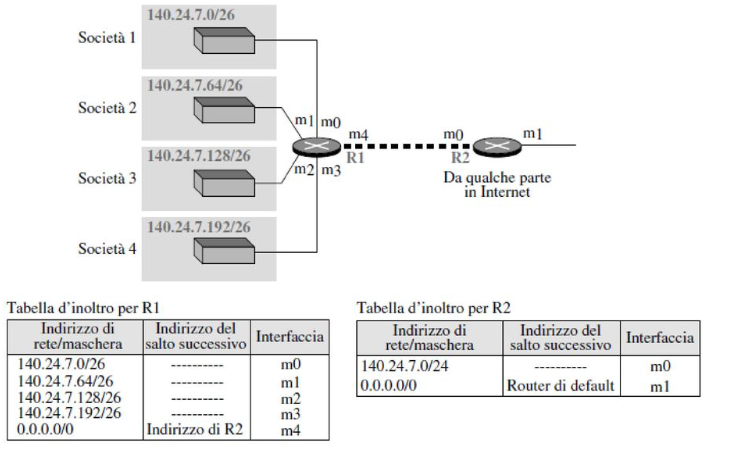
\includegraphics[width=0.7\textwidth]{images/es-aggregazione-indirizzi.PNG}
        %\captionof{figure}{Esempio}
    \end{minipage}
    
    E' evidente che R1 ha una tabella d'inoltro più lunga di R2 poiché ciascun datagramma che gli arriva deve essere indirizzato correttamente all'organizzazione appropriata. R2, invece, può avere una tabella d'inoltro molto piccola. Per R2, qualunque datagramma con indirizzo di destinazione compreso da \texttt{140.24.7.0} a \texttt{140.24.7.255} è inviato attraverso l'interfaccia m0, senza considerare in alcun modo il destinatario specifico (a quale organizzazione dovrà alla fine essere consegnato il datagramma). Questo meccanismo è chiamato aggregazione degli indirizzi, poiché i blocchi degli indirizzi di quattro società sono stati aggregati in un solo blocco più grande. Nel caso ciascuna organizzazione avesse blocchi di indirizzi che non possono essere aggregati in un blocco più grande (ad esempio blocchi non contigui), R2 sarebbe costretto ad avere una tabella d'inoltro molto più lunga.
\end{Example}

\subsubsection{Corrispondenza con la maschera più lunga}
Che cosa accade se una delle organizzazioni nella figura precedente non è geograficamente vicina alla altre tre? Ad esempio, se l'organizzazione 4 non può essere connessa al router R1 per qualche ragione, possiamo ancora utilizzare l'idea di aggregazione di indirizzo e assegnare il blocco \texttt{140.24.7.192/26} alla società 4? La risposa è si poiché l'instradamento nell'indirizzamento senza classi sfrutta un altro principio, la corrispondenza con la maschera più lunga (longest mask matching). Questo principio afferma che la tabella d'inoltro viene ordinata dalla maschera più lunga alla maschera più corta. In altre parole, se ci sono 3 maschere, /27, /26 e /24, la maschera /27 deve essere nella prima riga e la /24 deve essere nell'ultima (senza considerare la regola di default). 

\begin{Example}{Corrispondenza con la maschera più lunga}{}
    \textit{Vediamo se questo principio permette di risolvere la situazione nella quale l'organizzazione 4 è separata dalle altre tre.}

    \begin{minipage}{\textwidth}
        \centering
        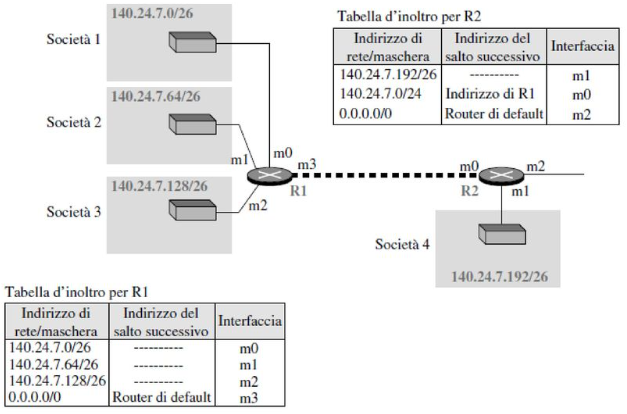
\includegraphics[width=0.6\textwidth]{images/es-corr-maschera.PNG}
        %\captionof{figure}{Esempio}
    \end{minipage}

    Supponiamo che un pacchetto arrivi al router R2 con indirizzo di destinazione \texttt{140.24.7.200}. La prima maschera nel router R2 è applicata e da l'indirizzo di rete \texttt{140.24.7.192}. Il datagramma è quindi instradato correttamente all'interfaccia m1 e raggiunge l'organizzazione 4. Tuttavia, se la tabella d'inoltro non fosse memorizzata con il prefisso più lungo per primo, applicando la maschera /24 si avrebbe un instradamento sbagliato e l'invio del datagramma al router R1.
\end{Example}

\subsection{ICMP}
L'IPv4 non implementa alcun meccanismo per segnalare gli errori o correggerli. Cosa accade se qualcosa va storto? Che cosa accade se un router deve scartare un datagramma perché non riesce a trovare un percorso per la destinazione finale o perché il campo time-to-live ha raggiunto il valore zero? Che cosa accade se un host di destinazione non ha ricevuto tutti i frammenti di un datagramma entro un determinato limite di tempo prestabilito? Queste sono tutte situazioni nelle quali si è verificato un errore, ma il protocollo IP non ha meccanismi integrati per renderlo noto all'host mittente.

Inoltre, il protocollo IP è sprovvisto di un meccanismo per effettuare richieste sullo stato di un sistema remoto. Ad esempio, un host, può a volte aver bisogno di determinare se un router o un altro host è attivo. Altre volte un amministratore di rete può aver bisogno di informazioni relative ad un host o un router.

Il protocollo ICMP (Internet Control Message Protocol) viene usato da host e router per scambiarsi informazioni a livello di rete: il suo uso più tipico è la notifica degli errori.

ICMP è spesso considerato parte di IP, ma dal punto di vista dell'architettura si trova esattamente sopra IP, dato che i suoi messaggi vengono trasportati nei datagrammi IP: ossia, i messaggi ICMP vengono trasportati come payload di IP, esattamente come i segmenti TCP o UDP. Allo stesso modo, se un host riceve un datagramma IP, che specifica ICMP come protocollo di livello superiore, allora effettua il demultiplexing dei contenuti del datagramma a ICMP, esattamente come farebbe per contenuti TCP o UDP.

\subsubsection{Messaggi}
I messaggi ICMP hanno un campo tipo e un campo codice e contengono l'intestazione e i primi 8 byte del datagramma IP che ha provocato la generazione del messaggio, in modo che il mittente possa determinare il datagramma che ha causato l'errore. Vengono mostrati alcuni tipi di messaggio ICMP:

\begin{center}
\begin{tabular}{|l|l|l|}
    \hline \textbf{Tipo ICMP} & \textbf{Codice} & \textbf{Descrizione}\\\hline
    0 & 0 & risposta echo (a ping)\\\hline
    3 & 0 & rete destinazione irraggiungibile\\\hline
    3 & 1 & host destinazione irraggiungibile\\\hline
    3 & 2 & protocollo destinazione irraggiungibile\\\hline
    3 & 3 & porta destinazione irraggiungibile\\\hline
    3 & 6 & rete destinazione sconosciuta\\\hline
    3 & 7 & host destinazione sconosciuto\\\hline
    4 & 0 & riduzione (controllo di congestione)\\\hline
    8 & 0 & richiesta echo\\\hline
    9 & 0 & annuncio di un router\\\hline
    10 & 0 & scoperta di un router\\\hline
    11 & 0 & TTL scaduto\\\hline
    12 & 0 & intestazione IP errata\\\hline
\end{tabular}
\end{center}

Una delle applicazioni che un host può utilizzare per verificare il funzionamento di un altro host è il programma ping. Il programma ping si basa sui messaggi di richiesta e risposta eco dell'ICMP. Un host invia una richiesta eco (tipo 8, codice 0) a un altro host che, se attivo, può rispondere con una risposta eco (tipo (0, codice 0). In maniera molto grossolana, il programma ping può anche misurare l'affidabilità e la congestione del router tra due host inviando una sequenza di messaggi richiesta-risposta.

\begin{Example}{Ping}{}
    \textit{Si mostra come inviare un messaggio ping al sito \texttt{pads.cs.unibo.it}. Il programma effettua automaticamente la risoluzione DNS del nome di dominio e inizializza il numero di sequenza a partire da 0: questo numero viene incrementato di uno ogni volta che viene inviato un nuovo messaggio di richiesta. Si noti che ping calcola il tempo di round-trip.}
    
    \texttt{
    \$ping pads.cs.unibo.it\\
    PING chernobog.pads.cs.unibo.it (130.136.132.11) 56(84) bytes of data.\\
    64 bytes from chernobog.pads.cs.unibo.it (130.136.132.11): icmp\_req=1 ttl=52 time=34.2 ms\\
    64 bytes from chernobog.pads.cs.unibo.it (130.136.132.11): icmp\_req=2 ttl=52 time=33.1 ms\\
    64 bytes from chernobog.pads.cs.unibo.it (130.136.132.11): icmp\_req=3 ttl=52 time=34.0 ms\\
    64 bytes from chernobog.pads.cs.unibo.it (130.136.132.11): icmp\_req=4 ttl=52 time=33.9 ms\\
    64 bytes from chernobog.pads.cs.unibo.it (130.136.132.11): icmp\_req=5 ttl=52 time=33.3 ms\\
    --- chernobog.puds.cs.unibo.it ping statistics ---\\
    5 packets transmitted, 5 received, 0\% packet loss, time 4005ms rtt min/avg/max/mdev = 33.177/33.758/34.220/0.417 ms
    }
\end{Example}

\subsubsection{Traceroute}
Il programma traceroute in UNIX o tracert in Windows può essere utilizzato per individuare il percorso di un datagramma dalla sorgente alla destinazione tramite l'identificazione dell'indirizzo IP di tutti i router che vengono visitati lungo il percorso. Solitamente il programma viene impostato per un massimo di 30 salti (router), che sono usualmente sufficienti per raggiungere la destinazione.

Il programma traceroute ha un funzionamento molto diverso da ping. Ping è basato su due messaggi query; traceroute è invece implementato per mezzo di due messaggi di segnalazione degli errori: tempo scaduto e destinazione non raggiungibile. Traceroute è un programma di livello di applicazione, ma in questo caso è necessario soltanto il programma client e non il server, poiché non è necessario raggiungere il livello di applicazione dell'host di destinazione. In altre parole non ci sono programmi server di traceroute. Il client traceroute genera un datagramma utente UDP usando intenzionalmente un numero di porta che, con alta probabilità, nel destinatario risulta inutilizzata. Se vi sono $n$ router nel percorso, il programma traceroute invia $(n + 1)$ datagrammi. I primi a messaggi vengono scartati dagli $n$ router, uno per ogni router, l'ultimo messaggio è scartato dall'host di destinazione. Il programma client traceroute utilizza $(n+1)$ messaggi ICMP di segnalazione degli errori per trovare il percorso tra sorgente e destinazione. 


\begin{Example}{Traceroute}{}
    \textit{Mostreremo che il programma traceroute non ha bisogno di conoscere il valore di n; esso viene trovato automaticamente. La figura mostra un esempio nel quale $n = 3$.}

    \begin{minipage}{\textwidth}
        \centering
        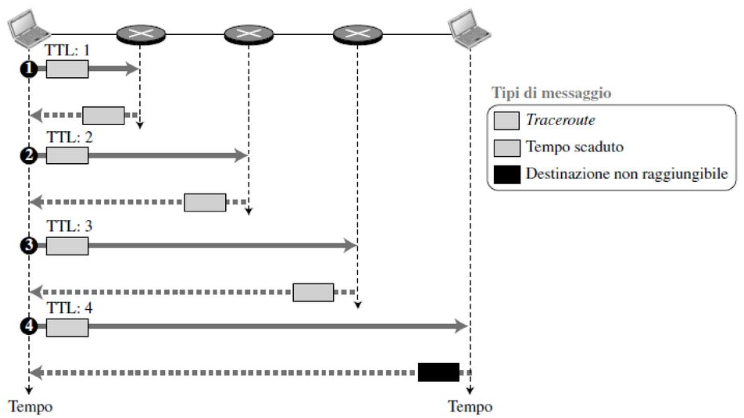
\includegraphics[width=0.7\textwidth]{images/es-traceroute.PNG}
        %\captionof{figure}{Esempio}
    \end{minipage}

    Il primo messaggio traceroute viene inviato con valore time-to-live (TTL) impostato a 1, il messaggio viene scartato quindi dal primo router e di conseguenza viene inviato un messaggio di errore ICMP di tempo scaduto. Grazie a quest'ultimo traceroute è in grado di determinare l'indirizzo IP del primo router (l'indirizzo IP del mittente del messaggio di errore) e il nome del router (che può essere presente nella sezione dati del messaggio). Il secondo messaggio traceroute è inviato con TTL impostato a 2, e il mittente può quindi trovare l'indirizzo IP e il nome del secondo router. Analogamente, il terzo messaggio permette di trovare le informazioni relative al router 3. Anche il quarto messaggio viene scartato quando raggiunge l'host di destinazione, ma per un'altra ragione. L'host di destinazione non trova alcuna applicazione in ascolto sulla porta di destinazione specificata nel datagramma utente UDP. Questa volta l'ICMP invia un messaggio diverso, il messaggio destinazione non raggiungibile con codice 3 (porta non raggiungibile), per indicare che non è stato possibile consegnare il datagramma. Dopo aver ricevuto questo messaggio ICMP diverso dai precedenti, il programma traceroute sa che la destinazione finale è stata raggiunta. Può quindi utilizzare le informazioni presenti nell'ultimo messaggio ICMP ricevuto per trovare l'indirizzo IP e il nome della destinazione finale.
\end{Example}

Il programma traceroute imposta inoltre un timer per trovare il tempo di round-trip di ciascun router e della destinazione. La maggior parte dei programmi traceroute invia tre messaggi a ogni dispositivo, con lo stesso valore di TTL, per poter effettuare una stima migliore del tempo di round-trip.

\section{Routing}
Instradare un pacchetto dalla sua sorgente alla sua destinazione significa pertanto instradare il pacchetto da un router sorgente (il router di default dell'host sorgente) a un router di destinazione (il router collegato alla rete di destinazione). Anche se un pacchetto deve passare attraverso i router sorgente e destinazione, la domanda è: quali altri router dovrà attraversare il pacchetto? In altre parole, poiché solitamente ci sono molti percorsi diversi tra la sorgente e la destinazione, quale percorso deve effettuare il pacchetto?

Per formulare i problemi di instradamento si utilizza un grafo. Ricordiamo che un grafo $G = (N,E)$ è un insieme $N$ di nodi e un insieme $E$ di archi (edge), ove ciascun arco collega una coppia di nodi di $N$. Nel contesto dell'instradamento a livello di rete, i nodi del grafo rappresentano i router – che prendono decisioni sull'inoltro dei pacchetti – e gli archi che connettono tali nodi rappresentano i collegamenti fisici tra i router.

\begin{figure}[ht]
    \centering
    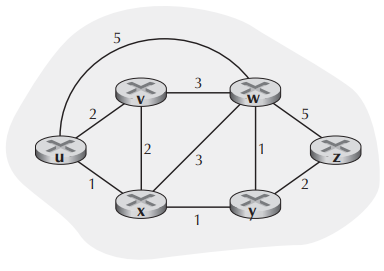
\includegraphics[width=7cm]{images/grafo.PNG}
    \caption{Modello astratto di un grafo di una rete di calcolatori}
    \label{fig:grafo}
\end{figure}

Un arco è anche associato un valore che ne indica il costo. In genere, questo può riflettere la lunghezza fisica del collegamento corrispondente (per esempio, un collegamento transoceanico può avere costo superiore rispetto a un collegamento terrestre a corto raggio), la velocità del collegamento o il suo prezzo. Per i nostri scopi, considereremo i costi degli archi come dati, senza preoccuparci di come siano stati determinati (spesso viene usato il termine metrica per indicare i costi associati agli archi di una rete). Per ogni arco $(x,y)$ tra i nodi $x$ e $y$ denotiamo con $c(x,y)$ il suo costo. Se la coppia $(x,y)$ non appartiene a $E$, poniamo $c(x,y) = +\infty$. Inoltre, consideriamo sempre e solo grafi non orientati, cioè con archi bidirezionali, ragion per cui l'arco $(x,y)$ è uguale all'arco $(y,x)$ e $c(x,y) = c(y,x)$. Inoltre, un nodo $y$ viene detto adiacente o vicino (neighbor) a un nodo $x$ se $(x,y)$ è un arco in $E$.

Dato che agli archi del grafo sono assegnati dei costi, obiettivo naturale di un algoritmo di instradamento è l'individuazione dei percorsi meno costosi tra sorgenti e destinazioni. Per rendere questo problema più preciso, ricordiamo che un percorso in un grafo $G = (N,E)$ è una sequenza di nodi $(x_1, x_2, ..., x_p)$ tali che ciascuna delle coppie $(x_1, x_2), (x_2, x_3), ..., (x_{p–1}, x_p)$ sia un arco appartenente a $E$. Il costo di un percorso $(x_1, x_2,..., x_p)$ è semplicemente la somma di tutti i costi degli archi lungo il percorso, ossia $c(x_1,x_2) + c(x_1, x_3) +...+ c(x_{p–1}, x_p)$. Dati due nodi qualsiasi $x$ e $y$, esistono più percorsi che li congiungono, ciascuno con il proprio costo. Uno o più di tali percorsi rappresenta un percorso a costo minimo (least-cost path). Il problema è quindi chiaro: determinare un percorso tra l'origine e la destinazione che abbia il costo minimo. Si noti che se tutti gli archi del grafo hanno lo stesso costo, il percorso a costo minimo rappresenta anche il percorso più breve (shortest path), ossia il percorso con il minor numero di collegamenti tra sorgente e destinazione.

\subsection{Algoritmi d'instradamento}
\subsubsection{Algoritmo d'instradamento con vettore distanza (Distance Vector - DV)}
L'instradamento distance-vector è iterativo, asincrono e distribuito. E' distribuito nel senso che ciascun nodo riceve parte dell'informazione da uno o più dei suoi vicini direttamente connessi, a cui, dopo aver effettuato il calcolo, restituisce i risultati. E' iterativo nel senso che questo processo si ripete fino a quando non avviene ulteriore scambio informativo tra vicini. E' asincrono nel senso che non richiede che tutti i nodi operino al passo con gli altri. Prima di presentare l'algoritmo usato dall'instramento DV sarà bene discutere un'importante relazione esistente tra costi e percorsi a costo minimo. Sia $d_x(y)$ il costo del percorso a costo minimo dal nodo $x$ al nodo $y$. Allora i costi minimi sono correlati dalla nota formula di Bellman-Ford:
\begin{equation*}
    d_x(y)=\min_v\{c(x,v)+d_v(y)\}
\end{equation*}
dove $\min_v$ riguarda tutti i vicini di $x$. Tale relazione è piuttosto intuitiva. Infatti se, dopo aver viaggiato da $x$ a $v$, consideriamo il percorso a costo minimo da $v$ a $y$, il costo del percorso sarà $c(x,v) + d_v(y)$. Dato che dobbiamo iniziare viaggiando verso qualche vicino $v$, il costo minimo da $x$ a $y$ è il minimo di $c(x,v) + d_v(y)$ calcolato su tutti i nodi adiacenti $v$.

\begin{Example}{Rappresentazione grafica dell'equazione di Bellman-Ford}{}
    \begin{minipage}{\textwidth}
        \centering
        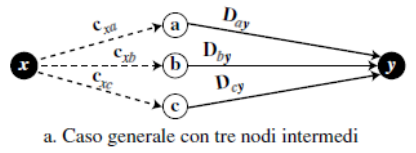
\includegraphics[width=0.5\textwidth]{images/es-bellman-ford.PNG}
        %\captionof{figure}{Esempio}
    \end{minipage}
    
    Possiamo pensare a $(a\to y)$, $(b\to y)$ e $(c\to y)$ come ai percorsi a costo minimo precedentemente stabiliti e a $(x\to y)$ come al nuovo percorso a costo minimo.
    \begin{equation*}
        D_{xy}=\min\{(c_{xa} + D_{ay} ), (c_{xb} + D_{by}), (c_{xc} + D_{cy})\}
    \end{equation*}
\end{Example}

Il concetto di vettore distanza è alla base del distance-vector routing. Un albero a costo minimo è una combinazione di percorsi a costo minimo dalla radice dell'albero verso tutte le destinazioni. Tali percorsi vengono collegati insieme per formare l'albero. Il routing a vettore distanza scinde questi percorsi e crea quello che viene chiamato un vettore distanza, cioè un array monodimensionale che rappresenta l'albero.

\begin{figure}[ht]
    \centering
    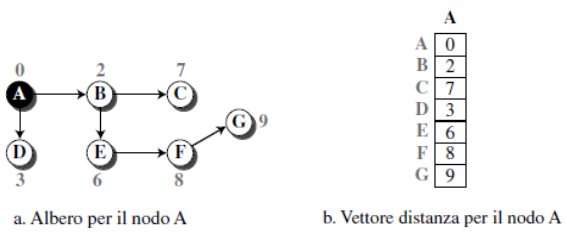
\includegraphics[width=9cm]{images/es-vettore-distanza.PNG}
    \caption{Il vettore a distanza che corrisponde ad un albero}
    \label{fig:es-vettore-distanza}
\end{figure}

Da notare che il "nome" del vettore distanza definisce la radice, gli indici invece definiscono le destinazioni e il valore di ogni cella definisce il costo minimo dalla radice alla destinazione. Un vettore distanza non fornisce il percorso da seguire per giungere alla destinazione (informazione che invece l'albero è in grado di fornire); il vettore riporta solo i costi minimi per le destinazioni.

Sappiamo che un vettore distanza può rappresentare i percorsi a costo minimo di un albero a costo minimo, ma la questione è: in quale modo i nodi all'interno di una rete all'inizio creano il proprio vettore distanza? Ogni nodo della rete, quando viene inizializzato, crea un vettore distanza molto rudimentale con le sole informazioni che il nodo riesce ad ottenere dai propri vicini (i nodi con cui è direttamente collegamento). Per fare questo, il nodo invia alcuni messaggi di benvenuto attraverso tutte le sue interfacce e scopre l'identità dei vicini e la sua distanza con ciascuno di essi. Quindi crea un semplice vettore distanza inserendo le distanze scoperte nelle celle corrispondenti e lascia il valore delle altre celle ad infinito. Questi vettori distanza rappresentano i percorsi a costo minimo elaborati sulla base delle sole informazioni (limitate) di cui dispone il nodo in questo momento. Quando si è a conoscenza di una sola distanza tra due nodi, questa può essere considerata il minimo. Per migliorare questi vettori, i nodi della rete devono aiutarsi scambiandosi informazioni. Dopo che ogni nodo ha creato il suo vettore ne invia una copia a tutti i suoi vicini. Quando un nodo riceve un vettore distanza da un vicino provvede ad aggiornare il suo vettore distanza applicando l'equazione di Bellman-Ford.

\begin{Example}{Vettori a distanza}{}
    \textit{Vengono mostrati i vettori a distanza iniziali della nostra rete:}

    \begin{minipage}{\textwidth}
        \centering
        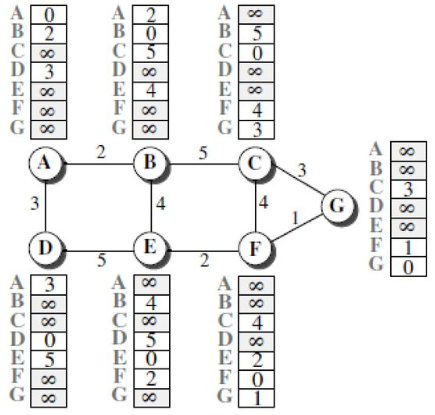
\includegraphics[width=0.4\textwidth]{images/es-vett-dist.PNG}
        %\captionof{figure}{Esempio}
    \end{minipage}

    Questi vettori iniziali non permettono veramente ad una rete di inoltrare i pacchetti. Per esempio il nodo A crede di non essere collegato al nodo G in quanto la cella corrispondente mostra un costo infinito.

    \begin{minipage}{\textwidth}
        \centering
        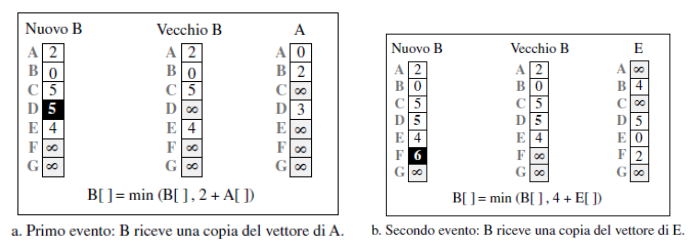
\includegraphics[width=0.7\textwidth]{images/es-vett-dist2.PNG}
        %\captionof{figure}{Esempio}
    \end{minipage}

    La figura mostra due eventi asincroni, che avvengono uno dopo l'altro, a distanza di qualche tempo. Nel primo evento il nodo A ha inviato il suo vettore al nodo B. Il nodo B aggiorna il suo vettore usando il costo $c_{BA}=2$. Nel secondo evento E ha inviato il suo vettore al nodo B. Il nodo B aggiorna il suo vettore usando il costo $c_{EA}=4$. Grazie al primo evento, il nodo B ha un miglioramento nel suo vettore: il suo costo minimo verso il nodo D è ora cambiato da infinito a 5 (passando attraverso il nodo A). Dopo il secondo evento il nodo B ha un ulteriore miglioramento del suo vettore: il suo costo minimo verso il nodo F è cambiato da infinito a 6 (passando attraverso il nodo E).
\end{Example}

Ora possiamo vedere lo pseudocodice semplificato che descrive l'algoritmo di routing basato su vettore a distanza. L'algoritmo viene eseguito da ogni nodo in modo indipendente e asincrono.

\begin{Algoritmo}{Algoritmo Distance Vector}{}
    L'idea di base è la seguente. Ciascun nodo $x$ inizia con $D_x(y)$, una stima del costo del percorso a costo minimo da se stesso al nodo $y$, per tutti i nodi in $N$. Sia \texttt{$D_x$ = [$D_x(y)$: y in N]} il vettore delle distanze del nodo $x$, che è il vettore delle stime dei costi da $x$ a tutti gli altri nodi, $y$, in $N$. Con l'algoritmo Bellman Ford, ciascun nodo $x$ mantiene i seguenti dati di instradamento. 
    \begin{itemize}
        \item Per ciascun vicino $v$, il costo $c(x,v)$ da $x$ al vicino $v$.
        \item Il vettore delle distanze del nodo $x$, che è \texttt{$D_x$ = [$D_x(y)$: y in N]}, contenente la stima presso $x$ del costo verso tutte le destinazioni, $y$, in $N$. 
        \item I vettori delle distanze di ciascuno dei suoi vicini, ossia \texttt{$D_v$ = [$D_v(y)$: y in N]}, per ciascun vicino $y$ di $x$.
    \end{itemize}
    
    In questo algoritmo distribuito e asincrono, di quando in quando un nodo invia una copia del proprio vettore delle distanze a ciascuno dei suoi vicini. Quando un nodo $x$ riceve un nuovo vettore da qualcuno dei suoi vicini $v$, lo salva e quindi usa la formula di Bellman-Ford per aggiornare il proprio vettore come segue:
    \begin{equation*}
    D_x(y) = \min_v\{c(x,v) + D_v(y)\} \textit{ per ciascun nodo y in N}
    \end{equation*}
    
    Se il vettore delle distanze del nodo $x$ è cambiato per via di tale passo di aggiornamento, il nodo $x$ manderà il proprio vettore aggiornato a ciascuno dei suoi vicini, i quali a loro volta aggiorneranno il proprio vettore.

    \begin{lstlisting}
    A ciascun nodo x:
    Inizializzazione
        per tutte le destinazioni y in N:
            se y e' un vicino
                Dx(y) = c(x, y)
            else
                Dx(y) = infinito
        per ciascun vicino w
            invia il vettore delle distanze Dx = [Dx(y): y in N] a w
    \end{lstlisting}
\end{Algoritmo}

Un problema con il routing basato su vettore distanza è che i decrementi di costo (cioè le buone notizie) si diffondono rapidamente, mentre gli aumenti di costo (le cattive notizie) si propagano lentamente. Affinché un protocollo di routing lavori correttamente, se un collegamento è rotto (e quindi il costo del relativo arco diventa infinito), ogni altro router dovrebbe venirne a conoscenza immediatamente, ma nel routing basato su vettore distanza serve un po' di tempo. Questo problema è spesso chiamato conteggio all'infinito. A volte servono molti aggiornamenti prima che il costo di un collegamento rotto venga registrato come infinito da tutti i router.

\begin{Example}{Conteggio all'infinito: ciclo a due nodi}{}
    \textit{Un esempio di conteggio all'infinito è il problema del ciclo a due nodi. Per comprendere il problema, diamo un'occhiata allo scenario illustrato.}

    \begin{minipage}{\textwidth}
        \centering
        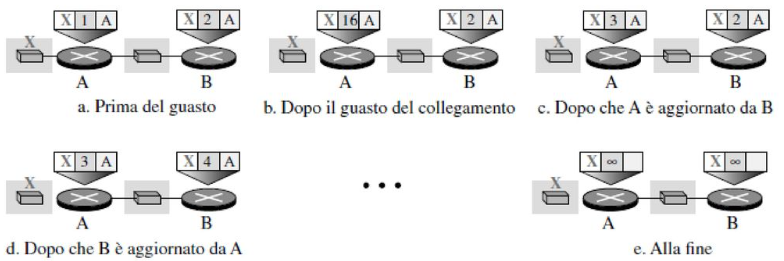
\includegraphics[width=0.8\textwidth]{images/es-instabilita-nodi.PNG}
        %\captionof{figure}{Esempio}
    \end{minipage}

    La figura illustra un sistema formato da tre nodi. Abbiamo mostrato solo le parti della tabella d'inoltro necessarie per la discussione. All'inizio sia il nodo A che il nodo B sanno come raggiungere il nodo X. Ma improvvisamente si guasta il collegamento tra A e X. Di conseguenza, il nodo A modifica la sua tabella. Se A invia immediatamente la sua tabella a B allora non c'è problema. Tuttavia, se B invia la sua tabella d'inoltro ad A prima ricevere quella di A, il sistema diventa instabile. Il nodo A riceve l'aggiornamento e, supponendo che B abbia trovato un modo per raggiungere X, aggiorna immediatamente la sua tabella d'inoltro. Ora A invia il suo nuovo aggiornamento a B. Quello che accade è che B è portato a credere che qualcosa sia cambiato vicino ad A e di conseguenza aggiorna la sua tabella d'inoltro. Il costo per raggiungere X aumenta gradualmente fino ad arrivare all'infinito. Ora, finalmente, sia A che B sanno che X non può essere raggiunto. Tuttavia, durante questo periodo di tempo il sistema non è stabile. Il nodo A crede che il percorso per raggiungere X passi da B e il nodo B crede che il percorso per raggiungere X passi attraverso A. Se A riceve un pacchetto destinato a X il pacchetto va a B e quindi ritorna ad A. Allo stesso modo, se B riceve un pacchetto destinato a X, va verso A e torna a B. I pacchetti rimbalzano tra A e B, creando un ciclo a due nodi.
\end{Example}

Una soluzione all'instabilità viene chiamata split horizon. Con questa strategia invece di inviare la tabella attraverso ogni interfaccia, ciascun nodo invia solo una parte della sua tabella tramite le sue varie interfacce. Se, secondo tale tabella, il nodo B ritiene che il percorso ottimale per raggiungere X passi tramite A, allora non deve fornire questa informazione ad A: l'informazione è arrivata da A che quindi la conosce già. Il fatto che le informazioni vengano prese dal nodo A, vengano modificate ed inviate nuovamente al nodo A è ciò che crea confusione. Nel nostro scenario, il nodo B elimina l'ultima riga della sua tabella d'inoltro prima di inviarla ad A. In questo caso il nodo A mantiene il valore di anche il nodo B corregge la sua tabella. Il sistema diventa stabile subito dopo il primo aggiornamento: sia il nodo A che il nodo B sanno che X non è più raggiungibile.

L'utilizzo della strategia split horizon ha un effetto collaterale. Normalmente il protocollo che implementa l'algoritmo di routing utilizza un timer: se per una certa quantità di tempo non ci sono novità circa un percorso, il nodo lo elimina dalla sua tabella. Quando il nodo B, nello scenario precedente, elimina il percorso verso X dai suoi annunci ad A, il nodo A non può sapere se ciò è dovuto alla strategia split horizon (la sorgente delle informazioni era A) o se dipende dal fatto che B recentemente non ha ricevuto alcuna notizia di X. Nella strategia dell'inversione avvelenata, B può ancora rendere pubblico il valore per X, ma se la sorgente delle informazioni è A, allora sostituisce la distanza con valore infinito. In questo caso l'infinito viene usato come avvertimento: "Non usare questo valore, quello che so circa questo percorso viene da te".

\subsubsection{Algoritmo d'instradamento a stato del collegamento (LS)}
Un algoritmo di routing che deriva direttamente dalla nostra precedente discussione sulla creazione degli alberi a costo minimo e delle tabelle d'inoltro è il routing a stato del collegamento, Link-State (LS) routing.

Questo metodo utilizza il termine link-state (stato del collegamento) per definire le caratteristiche di un collegamento (un arco) che rappresenta una rete, parte di una internet. In questo algoritmo, il costo associato ad un arco definisce lo stato del collegamento. I collegamenti con costi inferiori sono preferibili rispetto a quelli con costi superiori; se il costo di un collegamento è infinito, significa che esso non esiste più o è stato interrotto.

Per creare un albero a costo minimo utilizzando questo metodo ogni nodo deve avere una mappa completa della rete, il che significa che deve conoscere lo stato di ciascun collegamento. La raccolta di stati per tutti i collegamenti viene chiamata Link-State Database (LSDB). Il LSDB è unico per l'intera rete, ma ogni nodo deve averne un duplicato per poter essere in grado di creare l'albero a costo minimo. Il LSDB può essere rappresentato per mezzo di un array bidimensionale (matrice) in cui il valore di ogni cella definisce il costo del collegamento corrispondente.

\begin{figure}[ht]
    \centering
    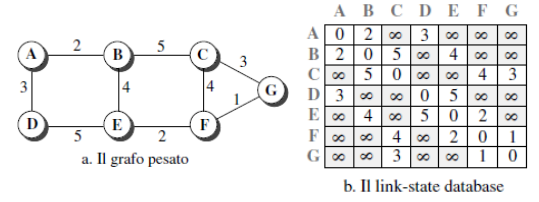
\includegraphics[width=10cm]{images/es-link-state-database.PNG}
    \caption{Esempio di un link-state database}
    \label{fig:es-link-state-database}
\end{figure}

Ora il problema è come può ogni nodo creare la sua copia del LSDB che contenga le informazioni necessarie sull'intera rete? Ciò può essere fatto tramite un procedimento chiamato flooding (inondazione). Ogni nodo può inviare dei messaggi di benvenuto a tutti i suoi vicini (i nodi ai quali è collegato direttamente) per raccogliere una coppia di informazioni circa ogni suo vicino: l'identità del nodo e il costo del collegamento. La combinazione di queste due informazioni viene chiamata pacchetto LS (LS packet, LSP). L'LSP viene inviato attraverso ogni interfaccia del nodo. Quando un nodo riceve un LSP da una delle sue interfacce e confronta il nuovo LSP con un'eventuale vecchia copia che potrebbe già avere. Se l'LSP appena arrivato è più vecchio di quello che ha già (questo è rilevabile confrontando i numeri di sequenza), l'LSP viene scartato. Se è più recente o è il primo ricevuto, il nodo scarta il vecchio LSP (se ce n'è uno) e conserva quello che ha appena ricevuto. A questo punto il nodo invia una copia dell'LSP da ogni sua interfaccia ad esclusione di quella da cui è arrivato il pacchetto. Questo garantisce che il flooding si interrompa da qualche parte nella rete (ad esempio dove un nodo ha una sola interfaccia). Dopo aver ricevuto tutti i nuovi LSP, ogni nodo è in grado di creare la sua copia dell'LSDB globale. Questo LSDB è esattamente uguale per ogni nodo e rappresenta l'intera mappa della rete.

\begin{figure}[ht]
    \centering
    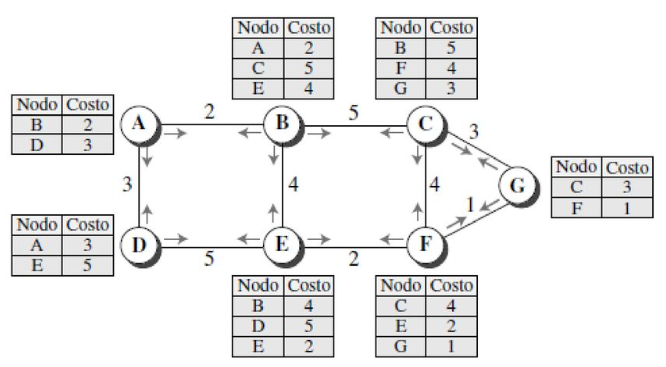
\includegraphics[width=10cm]{images/lsp-globale.PNG}
    \caption{Gli LSP creati ed inviati da ciascun nodo per costruire l'LSDB}
    \label{fig:lsp-globale}
\end{figure}

A questo punto possiamo confrontare l'algoritmo di routing a stato del collegamento con quello a vettore distanza. In quest'ultimo, ogni router comunica ai suoi vicini ciò che sa sull'intera rete, mentre nell'algoritmo di routing a stato del collegamento ogni router riferisce all'intera rete ciò che sa dei suoi vicini.

L'algoritmo di calcolo dei percorsi che presentiamo associato all'instradamento link state è noto come algoritmo di Dijkstra. L'algoritmo di Dijkstra calcola il percorso a costo minimo da un nodo (l'origine, che chiameremo $u$) a tutti gli altri nodi nella rete, è iterativo e ha le seguenti proprietà: dopo la $k$-esima iterazione, i percorsi a costo minimo sono noti a $k$ nodi di destinazione e, tra i percorsi a costo minimo verso tutti i nodi di destinazione, questi $k$ percorsi hanno i $k$ costi più bassi.

\begin{Algoritmo}{Algoritmo di Dijkstra}{}
    Per costruire il suo albero a costo minimo utilizzando I'LSDB condiviso, ogni nodo deve eseguire l'algoritmo di Dijkstra. Questo algoritmo è composto dai seguenti passi:
    \begin{itemize}
        \item il nodo sceglie se stesso come radice dell'albero, crea un albero con un singolo nodo e imposta il costo totale di ogni nodo sulla base delle informazioni che trova nell'LSDB;
        \item il nodo seleziona un altro nodo, tra tutti quelli che non sono presenti nell'albero, in modo che sia il più vicino possibile alla radice, e lo aggiunge all'albero. Dopo che questo nodo è stato aggiunto all'albero, il costo dei nodi non presenti nell'albero deve essere aggiornato in quanto i percorsi potrebbero essere cambiati;
        \item il nodo ripete il passaggio 2 finché tutti i nodi non sono stati aggiunti all'albero. I tre passaggi sopra riportati alla fine creano un albero a costo minimo.
    \end{itemize}
    
    Adottiamo la seguente notazione:
    \begin{itemize}
        \item $N$: insieme dei nodi della rete.
        \item $c(x,y)$: costo del collegamento dal nodo $x$ al nodo $y$.
        \item $D(v)$: costo minimo del percorso dal nodo origine alla destinazione $v$ per quanto concerne l'iterazione corrente dell'algoritmo.
        \item $p(v)$: immediato predecessore di $v$ lungo il percorso a costo minimo dall'origine a $v$.
        \item $N'$: sottoinsieme di nodi contenente tutti (e solo) i nodi $v$ per cui il percorso a costo minimo dall'origine a $v$ è definitivamente noto.
    \end{itemize}

    \begin{lstlisting}
    Inizializzazione:
    N' = {r} /* r e' la radice dell'albero */
    per tutti i nodi n
        se n e' adiacente a r
            allora D(n) = c(r,n)
        altrimenti D(n) = infinito

    Ciclo
    determina un n non in N' tale che D(n) sia minimo
    aggiungi n a N'
    per ogni nodo a adiacente a n e non in N' aggiorna D(a):
        D(a) = min(D(a), D(n) + c(n,a))
    /* il nuovo costo verso a e' il vecchio costo verso a oppure
    il costo del cammino minimo noto verso a piu' il costo da n a a */
    Finche' N' = N
    \end{lstlisting}
\end{Algoritmo}

\begin{Example}{Algoritmo di Dijkstra}{}
    \textit{Consideriamo la rete in figura e calcoliamo i percorsi a costo minimo da $u$ a tutte le destinazioni.} 
    
    \begin{minipage}{\textwidth}
        \centering
        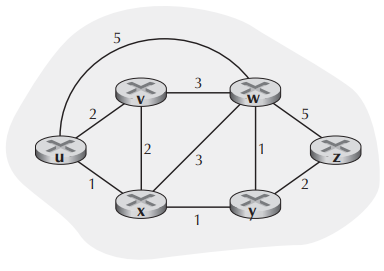
\includegraphics[width=0.4\textwidth]{images/grafo.PNG}
        %\captionof{figure}{Esempio}
    \end{minipage}
    
    I passi dell'algoritmo sono mostrati nella tabella, le cui righe forniscono i valori delle variabili dell'algoritmo al termine dell'iterazione. 

    \begin{center}
    \begin{tabular}{|l|l|l|l|l|l|l|}
        \hline\textbf{Passo} & \textbf{N'} & \textbf{D(v), p(v)} & \textbf{D(w), p(w)} & \textbf{D(x), p(x)} & \textbf{D(y), p(y)} & \textbf{D(z), p(z)}\\\hline
        0 & u & 2,u & 5,u & 1,u & $\infty$ & $\infty$\\\hline
        1 & ux & 2,u & 4,x &  &2,x & $\infty$\\\hline
        2 & uxy & 2,u & 3,y & & & 4,y\\\hline
        3 & uxyv &  & 3,y & & & 4,y\\\hline
        4 & uxyvw & & & & & 4,y\\\hline
        5 & uxyvwz & & & & &\\\hline
    \end{tabular}
    \end{center}
    
    Analizziamo in dettaglio i primissimi passi.
    \begin{itemize}
        \item Nel passo di inizializzazione i valori dei percorsi a costo minimo noti da $u$ ai suoi nodi adiacenti, $v$, $w$ e $x$, sono posti rispettivamente a 2, 5 e 1. In particolare il costo verso $w$ vale 5 (anche se vedremo presto che di certo esiste un percorso a costo inferiore) dato che questo è il costo del collegamento diretto (un solo hop) da $u$ a $w$. I costi verso $y$ e $z$ sono posti a infinito dato che tali nodi non sono adiacenti a $u$.
        \item Nella prima iterazione prendiamo in considerazione i nodi non ancora aggiunti all'insieme $N'$ e determiniamo il nodo a costo minimo come alla fine della precedente iterazione. Tale nodo è $x$, di costo 1, e pertanto $x$ viene aggiunto all'insieme $N'$. Viene poi aggiornato $D(v)$ per tutti i nodi, ottenendo i risultati mostrati nella seconda riga (Passo 1) della tabella. Il costo del percorso verso $v$ non è cambiato. Il costo del percorso verso $w$ (che era 5 al termine dell'inizializzazione) passando per il nodo $x$ è diventato 4. Viene quindi selezionato questo percorso a costo inferiore e il predecessore di $w$ lungo il percorso minimo da $u$ diventa $x$. Analogamente, il costo verso $y$ (attraverso $x$) viene calcolato essere 2, e la tabella viene aggiornata di conseguenza.
        \item Nella seconda iterazione si trova che i nodi $v$ e $y$ hanno percorsi a costo minimo (2), ne scegliamo arbitrariamente uno e aggiungiamo $y$ all'insieme $N'$ che ora conterrà $u$, $x$ e $y$. I costi verso i nodi rimanenti non ancora in $N'$, ossia $v$, $w$ e $z$, sono aggiornati dell'algoritmo Dijkstra, ottenendo i risultati mostrati nella terza riga della tabella.
        \item E così via...
    \end{itemize}
        
    Quando l'algoritmo Dijkstra termina, abbiamo per ciascun nodo il suo predecessore lungo il percorso a costo minimo dal nodo origine. Per ciascun predecessore abbiamo il rispettivo predecessore, e in questo modo riusciamo a costruire l'intero percorso dall'origine a tutte le destinazioni. La tabella di inoltro in un nodo, diciamo $u$, può pertanto essere costruita da queste informazioni memorizzando, per ciascuna destinazione, il nodo del successivo hop sul percorso a costo minimo da $u$ alla destinazione.

    \begin{minipage}{\textwidth}
        \centering
        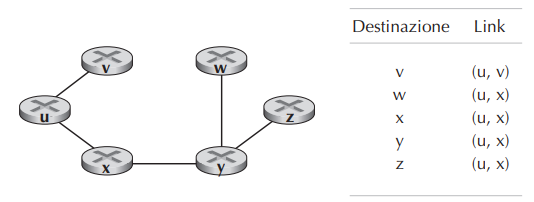
\includegraphics[width=0.6\textwidth]{images/es-dijkstra.PNG}
        \captionof{figure}{Percorso a costo minimo e tabella di inoltro per il nodo $u$}
    \end{minipage}
\end{Example}

\subsubsection{Confronto tra gli instradamenti LS e DV}
I due meccanismi di instradamento studiati utilizzano approcci complementari nel calcolare i percorsi. Nel DV ciascun nodo dialoga solo con i vicini direttamente connessi, informandoli delle stime a costo minimo da sé stesso a tutti i nodi (che conosce) nella rete. Nel LS, ciascun nodo dialoga con tutti gli altri nodi via broadcast, ma comunica loro solo i costi dei  collegamenti direttamente connessi. Concludiamo la nostra trattazione degli instradamenti LS e DV con un veloce confronto di alcuni dei rispettivi attributi. Ricordiamo che $N$ rappresenta l’insieme dei nodi (router) ed $E$ l’insieme degli archi (collegamenti).
\begin{itemize}
    \item \textit{Complessità dei messaggi.} LS richiede che ciascun nodo conosca il costo di ogni collegamento nella rete. Ciò implica l’invio di $O(|N|*|E|)$ messaggi. Inoltre, ogniqualvolta cambia il costo di un collegamento, il nuovo costo deve essere comunicato a tutti i nodi. A ogni iterazione l’instradamento DV richiede scambi di messaggi tra nodi adiacenti. Abbiamo visto che il tempo richiesto perché l’algoritmo converga può dipendere da molti fattori. Quando cambiano i costi dei collegamenti, l’instradamento DV propaga i risultati dei costi cambiati se il nuovo costo ha causato la variazione del percorso a costo minimo per uno o più nodi connessi a tale collegamento.
    \item \textit{Velocità di convergenza.} Abbiamo visto che la nostra implementazione di LS è un algoritmo $O(|N|^2)$ che richiede $O(|N|*|E|)$ messaggi. L’algoritmo del DV può convergere lentamente e può presentare cicli di instradamento. DV presenta anche il problema del conteggio all’infinito.
    \item \textit{Robustezza.} Che cosa avviene se un router si guasta, funziona male o viene sabotato? Con LS, un router può comunicare via broadcast un costo sbagliato per uno dei suoi collegamenti connessi (ma non per altri). Un nodo può anche alterare o eliminare i pacchetti ricevuti in broadcast LS. Ma i nodi LS si occupano di calcolare soltanto le proprie tabelle di inoltro, e gli altri nodi effettuano calcoli simili per quanto li riguarda. Ciò significa che i calcoli di instradamento sono in qualche modo isolati, il che fornisce un certo grado di robustezza. Con DV, un nodo può comunicare percorsi a costo minimo errati a tutte le destinazioni. Più in generale notiamo che, a ogni iterazione, il calcolo di DV in un nodo viene comunicato ai suoi vicini e quindi ai vicini dei vicini alla successiva iterazione. In questo senso, un calcolo errato su un nodo si può diffondere per l’intera rete.
\end{itemize}

In conclusione, nessuno dei due meccanismi di instradamento è nettamente superiore all’altro ed entrambi vengono utilizzati in Internet.

\subsubsection{Path-vector routing}
Sia il routing a stato del collegamento che a vettore distanza si basano sul costo minimo. Tuttavia, ci sono dei casi in cui il costo non è l'obiettivo prioritario. Ad esempio, supponiamo che nella rete ci siano dei router tramite i quali un mittente non vuole che passino i suoi pacchetti. Per esempio un router può appartenere ad una società che non fornisce un sufficiente livello di sicurezza o che appartiene a un rivale commerciale del mittente che potrebbe analizzare i pacchetti alla ricerca di informazioni riservate. Il routing a costo minimo non può evitare che un pacchetto transiti in un'area se tale area si trova lungo il percorso a costo minimo. In altre parole, lo scopo del costo minimo applicato dal routing LS o DV, non consente a un mittente di applicare politiche specifiche al percorso dei suoi pacchetti.

Per soddisfare queste richieste è stato ideato un terzo algoritmo di routing, chiamato path vector (PV) routing (routing a vettore-distanza). Il routing PV non ha gli svantaggi del routing LS o DV sopra descritti, in quanto non si basa sul routing a costo minimo. Il percorso migliore viene determinato dalla sorgente utilizzando la politica che essa stessa decide di imporre al percorso. In altre parole la sorgente può controllare il percorso.

Nel path-vector routing, il percorso da una sorgente a tutte le destinazioni viene determinato dal miglior albero di copertura (spanning tree). Esso, tuttavia, non è l'albero a costo minimo bensì è quello determinato dalla sorgente quando impone la propria politica. Se ci sono più percorsi per la destinazione, la sorgente può scegliere il percorso che corrisponde meglio a tale politica. Una sorgente è libera di applicare politiche multiple allo stesso tempo. Una delle politiche più comuni ho lo scopo di minimizzare il numero di nodi visitati. Un'altra politica comune è quella di imporre che i propri pacchetti non passino mai da alcuni nodi intermedi durante il loro percorso.

Il path-vector routing, come quello a vettore distanza, è un algoritmo di instradamento asincrono e distribuito. Gli alberi di copertura vengono creati gradualmente e in modo asincrono da ciascun nodo. Quando un nodo viene inizializzato, esso crea un path vector (vettore percorso) basato sulle informazioni che riesce ad ottenere dai suoi vicini. Anche in questo caso, un nodo invia dei messaggi di benvenuto ai suoi vicini per raccogliere tali informazioni. 

Ogni nodo, dopo la creazione del path-vector iniziale, lo invia a tutti i suoi vicini. Ogni nodo, quando riceve un path-vector da un vicino, aggiorna il suo path-vector tramite un'equazione simile a quella di Bellman-Ford, ma applicando la sua politica invece del costo minimo. Possiamo definire tale equazione come
\begin{equation*}
    percorso (x, y) = miglior \{percorso(x, y), [(x + percorso(v, y)]\} \textit{ per tutti i }v\textit{ nella rete}    
\end{equation*}

In tale equazione l'operatore ($+$) significa che bisogna aggiungere $x$ all'inizio del percorso. Dobbiamo anche essere cauti ed evitare di aggiungere un nodo a un percorso vuoto perché un percorso vuoto non è altro che un percorso inesistente. 

La politica viene definita selezionando il migliore tra vari percorsi. Il path-vector routing impone anche un'altra condizione a questa equazione: se il percorso $(v, y)$ comprende $x$, tale percorso viene scartato per evitare di aggiungere un ciclo. In altre parole $x$ non vuole visitare se stesso quando seleziona un percorso verso $y$.

\begin{Example}{Path vector routing}{}
    \textit{Viene mostrata una piccola rete con solo cinque nodi. Ogni sorgente ha creato il suo albero di copertura che corrisponde alla propria politica. La politica imposta da tutte le sorgenti è usare il numero minimo di nodi per raggiungere una destinazione.}

    \begin{minipage}{\textwidth}
        \centering
        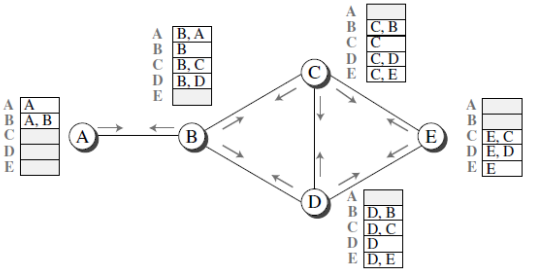
\includegraphics[width=0.6\textwidth]{images/es-path-vector.PNG}
        %\captionof{figure}{Percorso a costo minimo e tabella di inoltro per il nodo $u$}
    \end{minipage}

    E' bene notare che, anche in questo caso, non intendiamo dire che tutte queste tabelle vengono create simultanemente; esse vengono create quando i vari nodi vengono inizializzati. La figura mostra anche come questi path-vector vengono inviati ai vicini subito dopo che sono stati creati (le frecce in figura).

    \begin{minipage}{\textwidth}
        \centering
        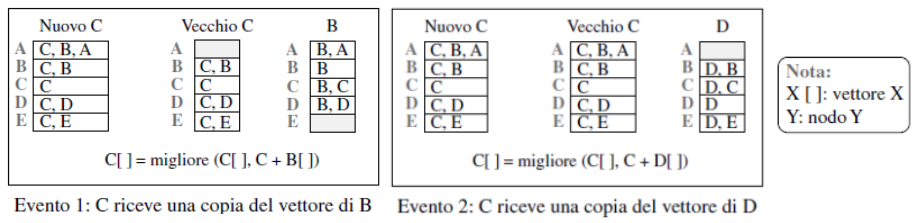
\includegraphics[width=0.9\textwidth]{images/es-path-vector2.PNG}
        %\captionof{figure}{Percorso a costo minimo e tabella di inoltro per il nodo $u$}
    \end{minipage}

    Viene mostrato il path-vector del nodo C dopo due eventi. Nel primo evento il nodo C riceve una copia del vettore B, che migliora il suo vettore: ora sa come raggiungere il nodo A. Nel secondo evento il nodo C riceve una copia del vettore D, che non cambia il suo vettore. Di fatto il vettore per il nodo C dopo il primo evento diviene stabile e serve da tabella d'inoltro.
\end{Example}

\begin{Algoritmo}{Algoritmo path-vector}{}
    Viene riportata una versione semplificata dell'algoritmo path-vector:
    \begin{lstlisting}
    Path Vector_Routing()
    {
        // Inizializzazione
        for (y = 1 to N)
        {
            if (y e' me stesso)
                Path[y] = me_stesso
            else if (y e' un vicino)
                Path[y] = me_stesso + il_nodo_vicino
            else
                Path[y] = vuoto
        }
        Spedisci il vettore (Path[1], Path[2],..., Path[y]} 
                                            a tutti i vicini
        // Aggiornamento
        repeat (sempre)
        {
            wait (un vettore Path, da un vicino w)
            for (y=1 to N)
            {
                if (Path comprende me_stesso)
                    scarta il percorso // Evita ogni ciclo
                else
                    Path[y] = il_migliore_tra [Path[y], 
                                (me_stesso + Path [y])]
            }
            If (c'e' un cambiamento nel vettore)
                Spedisci il vettore [Path[1], Path[2]..... Path[y]] 
                                                    a tutti i vicini
        }
    }// Fine del path-vector
    \end{lstlisting}
\end{Algoritmo}

\subsection{Protocollo di routing}
Un protocollo è qualcosa di più di un algoritmo. Un protocollo deve definire il suo ambito di
funzionamento, i messaggi che vengono scambiati, la comunicazione tra router e l’interazione con i protocolli di altri ambiti.

\subsubsection{Routing Information Protocol (RIP)}
Il Routing Information Protocol (RIP) è uno dei protocolli di routing intra-dominio più ampiamente utilizzati ed è basato sull'algoritmo di instradamento a vettore distanza.

La gestione dei costi viene gestita in modo molto semplice ed indipendentemente da fattori quali le prestazioni dei router e dei collegamenti, come ad esempio: ritardi, ampiezza della banda ecc. Quindi, il costo viene definito come il numero di salti (hop), cioè il numero di sottoreti, che un pacchetto deve visitare per andare dal router sorgente all'host di destinazione. Da notare che la rete nel quale si trova l'host sorgente non viene considerata in questo calcolo. Questo perché l'host sorgente non usa alcuna tabella d'inoltro: il pacchetto viene semplicemente consegnato al router di default. In RIP il costo massimo di un percorso è di 15 hop, il che significa che il valore 16 rappresenta l'infinito (nessuna connessione).

\begin{figure}[ht]
    \centering
    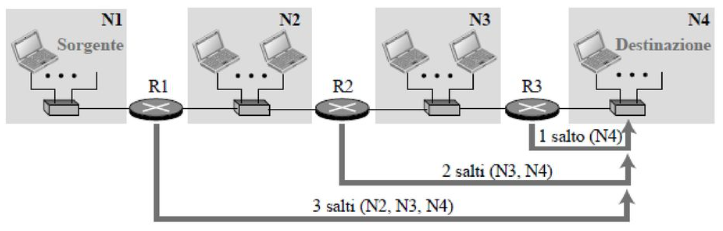
\includegraphics[width=11cm]{images/rip.PNG}
    \caption{Conto degli hop in RIP}
    \label{fig:rip}
\end{figure}

L'algoritmo a vettore distanza di cui abbiamo parlato ha lo scopo principale di scambiare vettori distanza tra i nodi vicini. Invece, in questo caso dei router il loro obiettivo è quello di costruire delle tabelle d'inoltro per far giungere i pacchetti alla loro rete di destinazione.

In RIP, una tabella d'inoltro è formata da tre colonne: nella prima c'è l'indirizzo della rete di destinazione, nella seconda l'indirizzo del prossimo router al quale il pacchetto deve essere inoltrato e nella terza il costo (numero di hop) per raggiungere la rete di destinazione. Si noti che la prima e la terza colonna insieme contengono le stesse informazioni di un vettore distanza, ma con la differenza che in questo caso il costo mostra il numero di salti fino alla rete di destinazione.

\begin{figure}[ht]
    \centering
    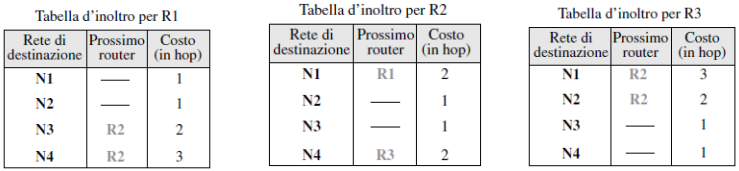
\includegraphics[width=11cm]{images/tabelle-rip.PNG}
    \caption{Tabelle d'inoltro}
    \label{fig:tabelle-rip}
\end{figure}

Anche se una tabella d'inoltro RIP definisce solo il prossimo router (nella seconda colonna), questa informazione è sufficiente per ricostruire l'intero albero minimo. Ad esempio R1 definisce che il prossimo router per il percorso verso N4 è R2; R2 definisce che il prossimo router per N4 è R3; R3 definisce che non c'è alcun router successivo per tale percorso. Quindi l'albero è $R1\to R2\to R3\to N4$.

Ci si potrebbe chiedere qual è l'uso della terza colonna della tabella d'inoltro. La terza colonna non è necessaria per inoltrare il pacchetto, ma serve per aggiornare la tabella d'inoltro quando ci sono modifiche del percorso.

RIP si basa su una coppia di processi, un client e un server, e sul loro scambio di messaggi. Una parte del messaggio, che chiamiamo voce (entry), può essere ripetuta tante volte quante necessarie. Ogni voce fornisce le informazioni relative a una riga della tabella d'inoltro del router che invia il messaggio.

\begin{figure}[ht]
    \centering
    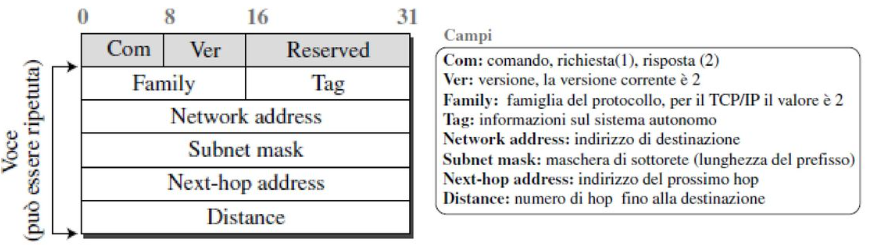
\includegraphics[width=11cm]{images/formato-messaggi-rip.PNG}
    \caption{Formato dei messaggi RIP}
    \label{fig:formato-messaggi-rip}
\end{figure}

Il RIP ha due tipi di messaggio: richieste e risposte. Un messaggio di richiesta viene inviato da un router appena acceso o da un router che ha delle voci scadute in memoria. I messaggi di richiesta possono riguardare voci specifiche oppure richiedere tutte le vocí disponibili. Un messaggio di risposta (o aggiornamento) può essere sollecitato o meno. Un messaggio di risposta sollecitato viene inviato solo come risposta a un messaggio di richiesta. Esso contiene informazioni circa la destinazione specificata nel messaggio di richiesta corrispondente. Un messaggio di risposta non sollecitato, invece, viene inviato periodicamente (ogni 30 secondi) o quando c'è un cambiamento nella tabella d'inoltro.

Per il suo funzionamento, RIP utilizza tre timer.
\begin{itemize}
    \item Il \textit{timer periodico} controlla l'invio dei messaggi di aggiornamento. Ogni router ha un timer periodico che viene impostato a un valore scelto casualmente nell'intervallo tra 25 e 35 secondi (per evitare che tutti i router inviino i loro messaggi allo stesso tempo e creino un picco di traffico). Il timer effettua il conto alla rovescia; quando arriva a zero viene inviato un messaggio d'aggiornamento e il timer viene impostato nuovamente in modo casuale. 
    \item Il \textit{timer di scadenza} regola la validità dei percorsi. Quando un router riceve delle informazioni aggiornate per un percorso, il timer di scadenza viene impostato a 180 secondi (per quel particolare percorso). Ogni volta che viene ricevuto un nuovo aggiornamento, il timer del relativo percorso viene fatto ripartire dal valore iniziale. Se ci sono dei problemi in una rete e non viene ricevuto alcun aggiornamento nell'arco dei 180 secondi assegnati, il percorso viene considerato come scaduto e il suo conto dei salti viene impostato a 16 (il che significa che la destinazione è irraggiungibile). 
    \item Il \textit{timer per la garbage collection} viene usato per eliminare i percorsi dalla tabella d'inoltro. Quando le informazioni circa un percorso non sono più valide, un router non provvede immediatamente alla loro rimozione dalla sua tabella. Al contrario, il router continua a annunciare il percorso con un valore di 16. Allo stesso tempo, per quel percorso, un timer per la garbage collection viene impostato a 120 secondi. Quando il contatore raggiunge lo 0, il percorso viene definitivamente eliminato dalla tabella. Questo timer consente ai vicini di venire a conoscenza di un percorso che non è più valido, prima che sia eliminato.
\end{itemize}

Analizziamo brevemente le caratteristiche di RIP:
\begin{itemize}
    \item \textit{Split horizon with poisoned reverse (inversione avvelenata).} Serve per evitare che un router invii rotte non valide al router da cui ha imparato la rotta (evitare cicli). Si mette a infinito (16) il costo della rotta che passa attraverso il vicino a cui si manda advertisement.
    \item \textit{Triggered updates.} Riduce il problema della convergenza lenta. Quando cambia una rotta si inviano immediatamente informazioni ai vicini senza attendere il timeout.
    \item \textit{Hold-down.} Fornisce robustezza. Quando si riceve una informazione di una rotta non più valida, si avvia un timer e tutti gli advertisement riguardanti quella rotta che arrivano entro il timeout vengono tralasciati.
\end{itemize}

Il RIP è implementato per mezzo di un processo demone (sempre attivo) che ascolta sulla porta nota 520 UDP. Nel caso di UNIX BSD tale processo viene chiamato routed (come abbreviazione di route daemon). Questo significa che anche se RIP è un protocollo di routing i messaggi RIP vengono incapsulati all'interno di datagrammi utente UDP, che a loro volta sono incapsulati in datagrammi IP. In altre parole, RIP lavora a livello di applicazione ma crea delle tabelle d'inoltro per IP (che si trova a livello di rete). Poiché RIP viene implementato come un processo a livello di applicazione, può inviare e ricevere messaggi su una socket standard e utilizzare un protocollo di trasporto standard.

\subsubsection{Open Shortest Path First (OSPF)}
Il termine open nell’acronimo indica che le specifiche del protocollo sono pubblicamente disponibili. 

OSPF è un protocollo link-state che utilizza il flooding (inondazione) di informazioni riguardo lo stato dei collegamenti e l’algoritmo di Dijkstra per la determinazione del percorso a costo minimo. In OSPF, un router costruisce una mappa topologica, cioè un grafo, dell’intero sistema autonomo e manda in esecuzione (locale) l’algoritmo di Dijkstra per determinare un albero dei percorsi minimi verso tutte le sottoreti (albero in cui il router stesso rappresenta il nodo radice). I costi dei collegamenti vengono fissati dall’amministratore di rete.

In OSPF, ogni qualvolta che si verifica un cambiamento nello stato di un collegamento (per esempio, una variazione di costo o un cambiamento di disponibilità), il router manda informazioni di instradamento via broadcast a tutti gli altri router nel sistema autonomo. Inoltre, invia periodicamente lo stato dei collegamenti (almeno ogni 30 minuti), anche se questo non è cambiato. Gli annunci OSPF sono contenuti in messaggi OSPF che vengono trasportati direttamente da IP come un protocollo di livello superiore con identificativo 89.

OSPF è un protocollo molto complesso che utilizza ben cinque tipi diversi di messaggi.
\begin{itemize}
    \item Il \textit{messaggio hello} (ciao) viene usato dai router per annunciare la propria esistenza e per indicare tutti gli altri nodi che sono già noti.
    \item Il \textit{messaggio database description} (descrizione database) viene normalmente inviato in risposta ad un messaggio hello per consentire a un router che si è appena connesso di ottenere l'intero LSDB. 
    \item Il \textit{messaggio link-state request} (richiesta stato del collegamento) viene inviato da un router che ha bisogno di informazioni su uno specifico collegamento. 
    \item Il \textit{messaggio link-state update} (aggiornamento stato del collegamento) è il messaggio principale usato da OSPF ed è essenziale per la costruzione dell'LSDB.
    \item Il \textit{messaggio di riscontro link-state} (link-state ack) viene usato per rendere affidabile OSPF: ogni router che riceve un messaggio di aggiornamento link-state deve darne riscontro al mittente.
\end{itemize}

\subsubsection{Struttura di Internet}
Prima di parlare dei protocolli di routing unicast dobbiamo comprendere la struttura attuale di Internet. La rete è cambiata, passando da una topologia ad albero, con un'unica dorsale (backbone), a una topologia con dorsali multiple gestite da aziende private.

\begin{figure}[ht]
    \centering
    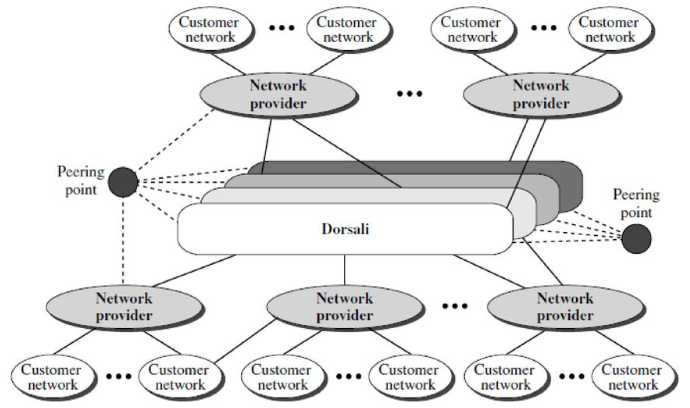
\includegraphics[width=11cm]{images/struttura-internet.PNG}
    \caption{Struttura di internet}
    \label{fig:struttura-internet}
\end{figure}

Ci sono numerose dorsali, gestite da società private di telecomunicazioni, che forniscono la connettività globale. Tali dorsali sono connesse tramite alcuni peering point che consentono la connettività tra dorsali. A livello inferiore, ci sono dei network provider (fornitori di rete) che utilizzano le dorsali per avere connettività globale ma principalmente forniscono servizi di connettività a clienti Internet. Infine ci sono le customer network (reti dei clienti) che usano i servizi forniti dai network provider. Tutte queste entità (dorsali, network provider o customer network) possono essere definite Internet Service Provider (ISP). In tutti e tre i casi forniscono dei servizi, ma a livelli differenti.

Nel nostro studio degli algoritmi di instradamento abbiamo visto la rete semplicemente come una collezione di router interconnessi. Ciascun router era indistinguibile dagli altri nel senso che tutti eseguivano lo stesso algoritmo per calcolare l’instradamento attraverso la rete. In pratica, questo modello con la sua visione omogenea dei router risulta un po’ semplicistico per almeno due importanti motivi.

\begin{itemize}
    \item \textit{Scalabilità.} Al crescere del numero di router, il tempo richiesto per calcolare, memorizzare e comunicare le informazioni di instradamento diventa proibitivo. Attualmente, Internet è costituita da centinaia di milioni di host. Archiviare le informazioni di instradamento su ciascuno di essi richiederebbe chiaramente un’enorme quantità di memoria, e il traffico generato dalla comunicazione broadcast degli aggiornamenti non lascerebbe banda per i pacchetti di dati. Un algoritmo distance-vector con interazioni tra un così grande numero di router non convergerebbe mai. Ovviamente, si deve fare qualcosa per ridurre la complessità del calcolo dei percorsi nelle reti di grandi dimensioni.
    \item \textit{Autonomia amministrativa.} Internet è una rete di ISP che generalmente desiderano gestire liberamente i propri router (per esempio, scegliendo l’algoritmo di instradamento preferito) o nascondere all’esterno aspetti dell’organizzazione interna della rete. L’ideale sarebbe che ciascuno fosse in grado di amministrare la propria rete nel modo auspicato, pur mantenendo la possibilità di connetterla alle reti esterne.
\end{itemize}

Implementare un routing gerarchico significa considerare ogni ISP come un sistema autonomo (Autonomous System, AS). Ogni AS può eseguire un protocollo di routing che soddisfa le sue esigenze. A livello di Internet globale, questo non è possibile: è necessario un protocollo di routing globale in grado di unire assieme tutti gli AS. Il protocollo di routing usato all'interno degli AS viene definito protocollo di routing intra-AS, protocollo di routing intradominio (intradomain routing protocol), o Interior Gateway Protocol (IGP); il protocollo di routing globale viene definito protocollo di routing inter-AS, protocollo di routing interdominio (interdomain routing protocol) o Exterior Gateway Protocol (EGP). Ci sono numerosi protocolli di routing intra-dominio, e ogni AS è libero di sceglierne uno, ma dovrebbe essere chiaro che dobbiamo avere un solo protocollo inter-dominio che gestisce il routing tra queste entità. Attualmente i due protocolli di routing intra-dominio più comuni sono RIP e OSPF; l'unico protocollo di routing inter-dominio è il BGP.

Come si è detto in precedenza, ogni ISP è un sistema autonomo quando si tratta di gestire le reti ed i router sotto il suo controllo. Anche se possono esserci AS piccoli, di medie dimensioni e grandi, ad ogni AS viene assegnato un numero identificativo (autonomous number, ASN) dall'ICANN. L'ASN è un numero intero senza segno, di 16 bit, che identifica in modo univoco l'AS. I sistemi autonomi, tuttavia, non sono classificati rispetto alla loro dimensione; vengono classificati a seconda del modo in cui sono connessi agli altri AS. Abbiamo degli AS stub (terminali), degli AS multihomed (a collegamenti multipli) e degli AS di transito. Il tipo, come vedremo in seguito, influenza il funzionamento del protocollo di routing inter-dominio rispetto all'AS.

\begin{itemize}
    \item \textit{AS stub.} Un AS stub ha un solo collegamento verso un altro AS. Il traffico dati può essere generato da o destinato ad un AS stub ma non può accadere che i dati transitino attraverso l'AS. Un buon esempio di AS stub è la rete di una grande azienda che può essere solamente sorgente o destinazione dei dati.
    \item \textit{AS multihomed.} Un AS multihomed ha più di una connessione con altri AS, ma non consente al traffico dei dati di passare attraverso di esso. Un buon esempio di questo tipo di AS è quello di un'azienda che può usare i servizi di più di un network provider ma come politica impone che gli AS a cui è collegata non possano sfruttare la sua rete per il transito dei loro dati.
    \item \textit{AS di transito.} Un AS di transito è collegato a vari AS e consente anche il transito del traffico dati. I network provider e le dorsali sono dei buoni esempi di AS di transito.
\end{itemize}

\subsubsection{Border Gateway Protocol (BGP)}
Il border gateway protocol, detto BGP, rappresenta l’attuale standard de facto dei protocolli di instradamento tra sistemi autonomi in Internet. BGP è forse il più importante dei protocolli di Internet, al pari di IP, in quanto è la colla che tiene insieme le migliaia di ISP che formano Internet. E' un protocollo di tipo distance-vector decentralizzato e asincrono.

BGP mette a disposizione di ciascun router un modo per:
\begin{enumerate}
    \item Ottenere informazioni sulla raggiungibilità dei prefissi di sottorete da parte dei sistemi confinanti. In particolare, BGP consente a ciascuna sottorete di comunicare la propria esistenza al resto di Internet. Basta che una sottorete urli “Esisto, son qui” e BGP si assicura che lo sappiano tutti i router di Internet. Se non fosse per BGP, ogni sottorete sarebbe isolata, sola, sconosciuta e irraggiungibile dal resto di Internet.
    \item Determinare i percorsi “ottimi” verso le sottoreti. Un router può venire a conoscenza di più cammini verso uno specifico prefisso; per determinare il migliore, esegue localmente BGP, sulla base delle informazioni di raggiungibilità e delle politiche del sistema.
\end{enumerate}

Per permettere ad ogni router di instradare correttamente i pacchetti, qualsiasi sia la destinazione, è necessario installare su tutti i router di confine (border router) dell'AS una variante del BGP chiamata BGP esterno (external BGP, eBGP). Tutti i router (non solamente quelli di confine) dovranno invece usare la seconda variante del BGP, chiamata BGP interno (internal BGP, iBGP). Questo significa che i router di confine devono eseguire ben tre protocolli d'instradamento (intra-dominio, eBGP e iBGP) e che tutti gli altri router ne eseguono due (intra-dominio e iBGP).



\begin{Example}{eBGP e iBGP}{}
    \textit{Si consideri la rete in figura con tre AS: AS1, AS2 e AS3, quest’ultimo con una sottorete di prefisso x.}

    \begin{minipage}{\textwidth}
        \centering
        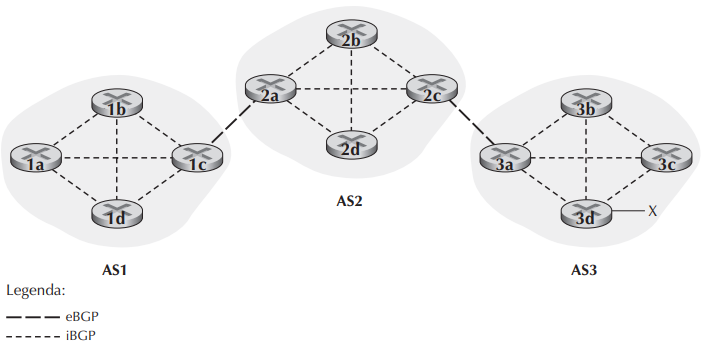
\includegraphics[width=0.7\textwidth]{images/es-eBGP-iBGP.PNG}
        %\captionof{figure}{Percorso a costo minimo e tabella di inoltro per il nodo $u$}
    \end{minipage}

    Ogni router, in ogni AS, funge sia da router gateway, vale a dire un router di bordo direttamente connesso a uno o più router in altri AS, sia da router interno, connesso cioè solo a host e router interni all’AS. In AS1, per esempio, il router 1c è un router gateway, mentre 1a, 1b e 1d sono router interni.

    Esaminiamo ora come BGP distribuirebbe le informazioni di raggiungibilità del prefisso x a tutti i router. In linea di principio è semplice. AS3 invia un messaggio BGP ad AS2, con l’annuncio dell’esistenza in AS3 di x; denotiamo tale messaggio con “AS3 x”. Quindi AS2 invia un messaggio BGP a AS1 con l’annuncio che x esiste ed è raggiungibile passando prima da AS2 per poi arrivare a AS3: “AS2 AS3 x”. In questo modo ogni AS verrà a conoscenza non solo dell’esistenza di x ma anche dei percorsi per raggiungerlo.

    Benché questa sia l’idea generale, in realtà sono i router e non gli AS a inviare gli annunci. In BGP, coppie di router si scambiano informazioni di instradamento su connessioni TCP semi-permanenti usando la porta 179. Ogni connessione TCP, con tutti i messaggi BGP che vi vengono inviati, è detta sessione BGP. Nel caso in cui questa coinvolga due sistemi autonomi viene detta sessione BGP esterna (sessione eBGP), mentre quella tra router dello stesso sistema autonomo è chiamata sessione BGP interna (sessione iBGP).
    Generalmente, in BGP c’è una connessione TCP di questo tipo per ciascun collegamento che connette direttamente due router in due diversi sistemi autonomi; nella figura vediamo una connessione sessione eBGP tra i gateway 2a e 1c e tra i router 2c e 3a.

    Esaminiamo ora come BGP distribuirebbe le informazioni di raggiungibilità del prefisso x ad AS1 e AS2. In router gateway 3a invia un messaggio eBGP “AS3 x” al router gateway 2c che a sua volta lo invia su una sessione iBGP a tutti i router di AS2 compreso il gateway 2a. Quest’ultimo quindi invia un messaggio eBGP “AS2 AS3 x” al router gateway 1c, che infine usa iBGP per inviare il messaggio “AS2 AS3 x” a tutti i router di AS1. Completato tale processo, ogni router di AS1 e AS2 è a conoscenza dell’esistenza di x e del percorso per raggiungerlo. Ovviamente in una rete reale esistono più percorsi da un router a una data destinazione che attraversano AS diversi.
\end{Example}

Il BGP è un protocollo sostanzialmente punto-punto. Quando il software BGP viene installato in due router, essi cercano di creare una connessione TCP utilizzando la porta nota 179. In altre parole si forma una coppia client/server che continua a scambiarsi messaggi. I due router che eseguono i processi BGP vengono chiamati peer BGP oppure speaker BGP.

La variante eBGP del BGP permette a due router di confine che si trovano in due diversi AS di formare coppie di speaker eBGP e di scambiarsi messaggi. Ogni connessione logica nella terminologia BGP viene definita sessione. 

\begin{Example}{Funzionamento di eBGP}{}\label{funzionamento-eBGP}
    \textit{Nel nostro esempio ci sono tre sessioni, come mostrato in figura.}

    \begin{minipage}{\textwidth}
        \centering
        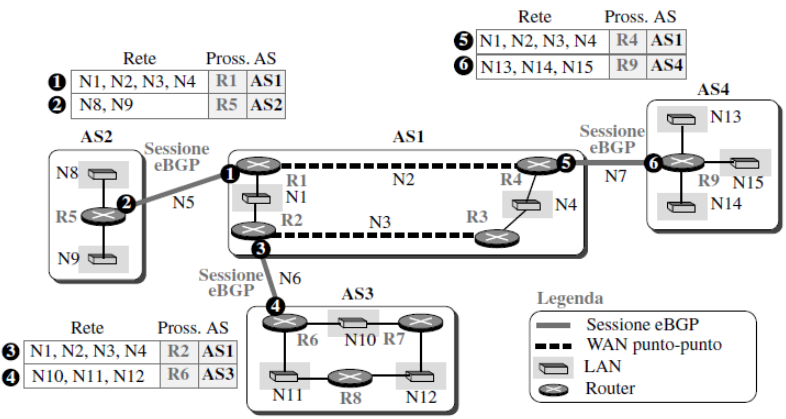
\includegraphics[width=0.8\textwidth]{images/funzionamento-eBGP.PNG}
        %\captionof{figure}{Percorso a costo minimo e tabella di inoltro per il nodo $u$}
    \end{minipage}

    La figura mostra anche i messaggi di aggiornamento (in versione molto semplificata) inviati dai router coinvolti nelle sessioni eBGP. Caso per caso, il numero cerchiato indica il router mittente del messaggio. Ad esempio, il messaggio numero 1 viene inviato dal router R1 e dice al router R5 che N1, N2, N3 ed N4 sono reti che possono essere raggiunte tramite il router R1 (R1 trae questa informazione dalla sua tabella d'inoltro intra-dominio). Il Router R5 ora può aggiungere queste informazioni in coda alla sua tabella d'inoltro. Quando R5 riceve un qualsiasi pacchetto destinato ad una di queste quattro reti può usare la sua tabella d'inoltro e scoprire che il prossimo router a cui inviare il pacchetto è R1.    
\end{Example}

E' facile notare che i messaggi scambiati durante le tre sessioni eBGP servono per indicare ad alcuni router come instradare i pacchetti destinati ad alcune reti nella internet, ma le informazioni di raggiungibilità non sono complete. Ci sono due problemi che devono ancora essere affrontati.
\begin{enumerate}
    \item Alcuni router di confine non sanno come instradare un pacchetto destinato ad un AS che non è un vicino. Ad esempio, R5 non sa come instradare i pacchetti destinati alle reti in AS3 e AS4. I router R6 ed R9 si trovano nella stessa situazione di R5, infatti R6 non sa  nulla delle reti in AS4 e R9 non sa nulla delle reti in AS3. 
    \item Nessuno dei router non di confine sa come instradare un pacchetto destinato alle reti che si trovano in altri AS.
\end{enumerate}

Per risolvere questi due problemi dobbiamo vedere l'uso della seconda variante del protocollo BGP, l'iBGP, che a differenza dell'eBGP viene eseguito tra tutte le coppie di router (di confine e non).

Il protocollo iBGP è simile al protocollo eBGP per il fatto che utilizza anch'esso connessioni TCP su porta nota 179. Ma a differenza di eBGP crea una sessione tra ogni possibile coppia di router all'interno di un AS. Tuttavia vanno chiariti alcuni punti. Per prima cosa, se un AS ha un solo router ovviamente non può esserci alcuna sessione iBGP. Infatti, nella nostra rete d'esempio, non possiamo creare una sessione iBPG all'interno di AS2 o AS4. In secondo luogo, se ci sono $n$ router in un AS, saranno generate $[n(n-1)/2]$ sessioni iBGP interne all'AS. 

\begin{Example}{Combinazione di sessioni eBGP e iBGP}{}
    \textit{Viene mostra la combinazione delle sessioni eBGP e iBGP nell'esempio.}

    \begin{minipage}{\textwidth}
        \centering
        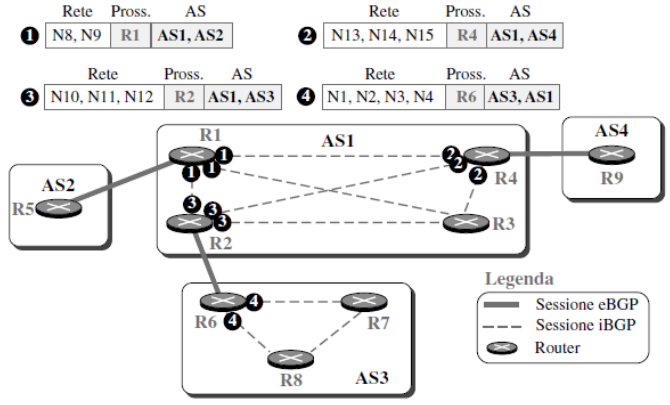
\includegraphics[width=0.7\textwidth]{images/combinazione-eBGP-iBGP.PNG}
        %\captionof{figure}{Percorso a costo minimo e tabella di inoltro per il nodo $u$}
    \end{minipage}

    Da notare che non è stato necessario mostrare in figura le reti fisiche all'interno degli AS visto che le sessioni BGP sfruttano normali connessioni TCP. Inoltre, è interessante notare anche che in questa fase vengono scambiati solo quattro messaggi. Il primo messaggio (numero 1) viene inviato da R1 e rende noto che le reti N8 e N9 sono raggiungibili tramite il percorso AS1-AS2, e il router successivo è R1. Il messaggio viene inviato, tramite sessioni separate, a R2, R3 ed R4. I router R2, R4 e R6 fanno la stessa cosa ma inviano messaggi diversi a destinazioni diverse. Il punto interessante è che, in questa fase, R3, R7 ed R8 creano delle sessioni con i loro peer, ma in realtà non hanno alcun messaggio da inviare.

    Il processo d'aggiornamento non termina qui. Per esempio, dopo che R1 ha ricevuto il messaggio d'aggiornamento da R2, esso combina le informazioni circa la raggiungibilità di AS3 con quelle che già conosceva relativamente ad AS1 ed invia un nuovo messaggio d'aggiornamento a R5. Ora R5 sa come raggiungere le reti in AS1 e AS3. Il processo continua quando R1 riceve il messaggio d'aggiornamento da R4. 
\end{Example}

A un certo punto è necessario che non vi siano più modifiche agli aggiornamenti ricevuti in precedenza e che tutte le informazioni siano state propagate attraverso tutti gli AS. Ora ogni router può combinare le informazioni ricevute dall'eBGP e dall'iBGP e creare una tabella dei percorsi, ma solo aver applicato il criterio scelto per trovare il percorso migliore. 

\begin{Example}{Tabelle di percorso}{}\label{tabelle-percorso}
    \textit{Vengono mostrate le tabelle di percorso per i router dell'esempio.}

    \begin{minipage}{\textwidth}
        \centering
        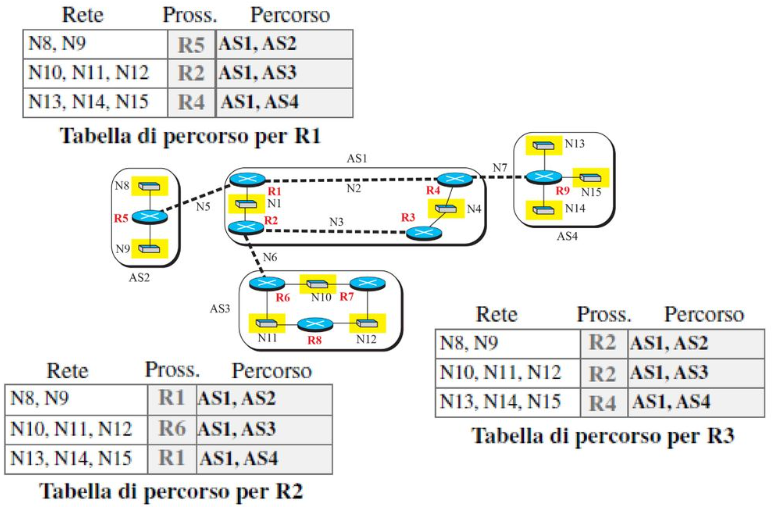
\includegraphics[width=0.7\textwidth]{images/tabelle-percorso.PNG}
        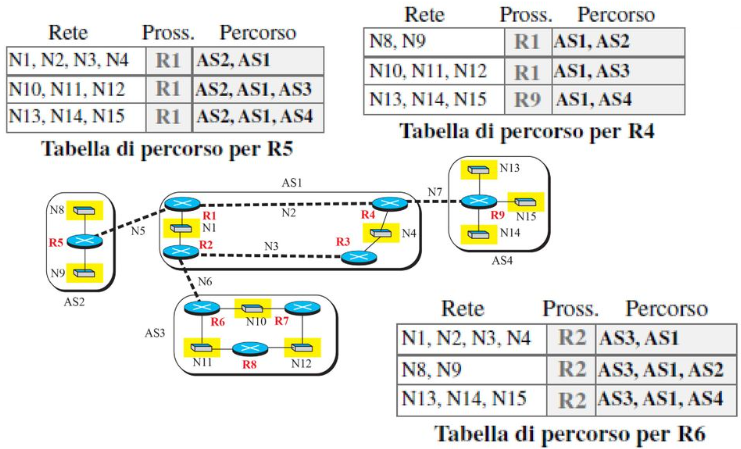
\includegraphics[width=0.7\textwidth]{images/tabelle-percorso2.PNG}
        %\captionof{figure}{Percorso a costo minimo e tabella di inoltro per il nodo $u$}
    \end{minipage}
    
    Per esempio il router R1 ora sa che tutti i pacchetti destinati alle reti N8 o N9 dovranno passare attraverso AS1 e AS2 e il router successivo a cui inoltrare il pacchetto è il router R5. Allo stesso modo, il router R4 sa che ogni pacchetto destinato alle reti N10, N11 ed N12 deve passare tramite AS1 e AS3 e il router successivo a cui inoltrare questo pacchetto è il router R1, ecc.    
\end{Example}

Il ruolo di un protocollo d'instradamento inter-dominio come il BGP è quello di permettere ai router all'interno dell'AS di incrementare le loro informazioni di routing. In altre parole, le tabelle di percorso ottenute ed organizzate da BPG non vengono usate, di per sé, per l'instradamento dei pacchetti. Bensì sono inserite nelle tabelle d'inoltro intra-dominio (generate RIP - OSPF). Ciò può essere fatto in molti modi, a seconda del tipo di AS.

Nel caso di AS stub, l'unico router di confine dell'area aggiunge una regola di default alla fine della sua tabella d'inoltro e definisce come prossimo router quello (detto speaker) che si trova dall'altro lato della connessione eBGP. Nell'Esempio \ref{funzionamento-eBGP}, R5 in AS2 definisce l'R1 come router di default per tutte le reti diverse da N8 ed N9. La situazione è la stessa per il router R9 in AS4 con il router di default impostato su R4. In AS3, R6 imposta R2 come suo router di default, mentre R7 e R8 impostano R6. Queste impostazioni avvengono in conformità con le tabelle di percorso descritte nell'Esempio \ref{tabelle-percorso} per tali router. In altre parole le tabelle di percorso vengono inserite nelle tabelle d'inoltro intra-domino aggiungendo una sola ulteriore regola di default.

Nel caso di un AS di transito la situazione è più complicata. R1 in AS1 deve inserire l'intero contenuto della tabella di percorso per R1 (Esempio \ref{tabelle-percorso}) nella sua tabella d'inoltro intra-dominio. La situazione è la stessa per R2, R3 ed R4.

Un problema da risolvere è il valore da associare al costo. Sappiamo che RIP e OSPF usano metriche differenti. Una soluzione molto comune è quella di impostare il costo di tutte le reti esterne allo stesso costo necessario per raggiungere il primo AS nel percorso. Ad esempio, il costo di R5 per raggiungere tutte le reti negli altri AS è pari al costo per raggiungere N5. Il costo di R1 per raggiungere le reti N10, N11 e N12 è il costo per raggiungere N6, e così via. Quindi, in questo caso, il costo viene preso direttamente dalle tabelle d'inoltro intra-dominio.

\begin{Example}{Tabelle d'inoltro inter-dominio}{}
    \textit{Vengono mostrate le tabelle d'inoltro inter-dominio.}

    \begin{minipage}{\textwidth}
        \centering
        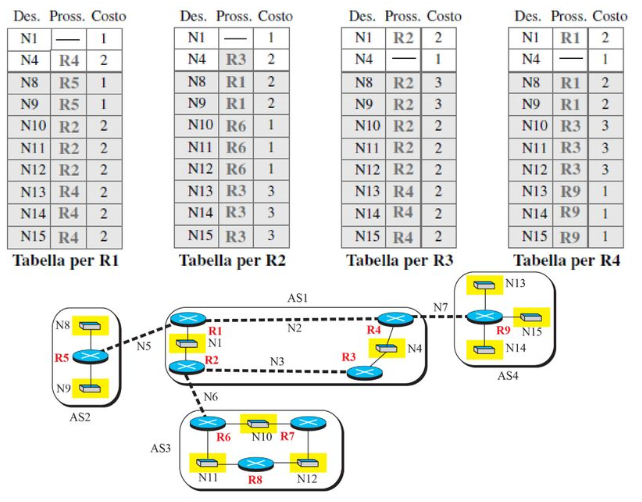
\includegraphics[width=0.7\textwidth]{images/tabelle-inoltro.PNG}
        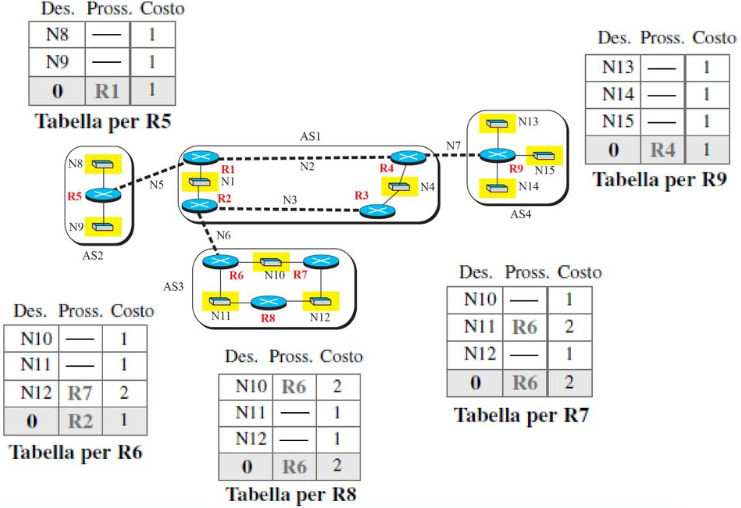
\includegraphics[width=0.7\textwidth]{images/tabelle-inoltro2.PNG}
        %\captionof{figure}{Percorso a costo minimo e tabella di inoltro per il nodo $u$}
    \end{minipage}

    Per semplicità assumiamo che tutti gli AS stiano utilizzando il RIP come protocollo di routing intra-dominio. Le aree ombreggiate sono le informazioni inserite dal protocollo BGP, le regole di default hanno il valore 0 come destinazione.
\end{Example}

Quando un router annuncia un prefisso per una sessione BGP, include anche un certo numero di attributi BGP. In gergo, un prefisso assieme ai suoi attributi è detto rotta (route). Due dei più importanti attributi sono AS-PATH e NEXT-HOP. 

AS-PATH elenca i sistemi autonomi attraverso i quali è passato l’annuncio del prefisso. Quando un prefisso attraversa un sistema autonomo, questi aggiunge il proprio ASN all’attributo AS-PATH. I router usano tale attributo per rilevare ed evitare gli annunci reiterati. Nello specifico, se un router vede che il proprio AS è contenuto nella lista di percorsi, rifiuta l’annuncio.

Nel fornire il delicato collegamento tra i protocolli di instradamento intra-AS e inter-AS, l’attributo NEXT-HOP ha un ruolo sottile, ma importante. In NEXT-HOP è riportata l’interfaccia del router che inizia l’AS-PATH.

L’input del processo di selezione è l’insieme di tutte le rotte apprese e accettate dal router. Se ne esistono due o più verso lo stesso prefisso, BGP invoca in sequenza le seguenti regole di eliminazione fino a individuare un’unica possibilità.
\begin{enumerate}
    \item Alle rotte viene assegnato come attributo un valore di preferenza locale, che potrebbe esser stato impostato direttamente dal router o appreso da un altro router nello stesso AS. Si tratta di una scelta che è lasciata all’amministratore di rete del sistema autonomo. Si selezionano quindi le rotte con i più alti valori di preferenza locale.
    \item Tra le rotte con lo stesso valore di preferenza locale, si seleziona quella con AS-PATH più breve. Se questa fosse l’unica regola di selezione, allora BGP utilizzerebbe un algoritmo Bellman Ford per la determinazione del percorso, con metrica sulla distanza data dal numero di hop tra sistemi autonomi anziché il numero di hop tra router.
    \item Tra le rotte con lo stesso valore di preferenza locale e la stessa lunghezza AS-PATH si seleziona quella il cui router di NEXT-HOP è più vicino. In questo caso, con “router più vicino” s’intende quello che presenta il percorso con costo minore, determinato dall’algoritmo intra-AS (instradamento a patata bollente).
    \item Se rimane ancora più di una rotta, il router si basa sugli identificatori BGP.
\end{enumerate}

Il protocollo BGP usa quattro tipi di messaggi per la comunicazione tra speaker, sia attraverso gli AS che all'interno di un AS: open (apertura), update (aggiornamento), keepalive (mantenimento in vita) e notification (notifica). Tutti i pacchetti BGP condividono la stessa intestazione comune.
\begin{itemize}
    \item \textit{Messaggio open.} Per collegarsi ai router vicini, un router BGP apre una connessione TCP con un vicino ed invia un messaggio di questo tipo.
    \item \textit{Messaggio update.} Si tratta del cuore del protocollo BGP. I messaggi di update sono usati dai router per rimuovere le destinazioni che erano state precedentemente annunciate, per annunciare il percorso verso una nuova destinazione, o entrambe le cose. Da notare che in BGP, un singolo messaggio di update può rimuovere numerose destinazioni già annunciate in precedenza ma può annunciare solo una nuova destinazione (o destinazioni multiple con gli stessi attributi di percorso).
    \item \textit{Messaggio keepalive.} I peer BGP si scambiano, a intervalli regolari di tempo, dei messaggi per verificare che il peer dall'altro lato della connessione sia ancora presente e funzionante.
    \item \textit{Messaggio notification.} Un messaggio di notifica viene inviato da un router ogni volta che una condizione d'errore viene rilevata oppure se un router desidera chiudere la sessione.
\end{itemize}

\subsection{Routing multicast}
Nelle sezioni precedenti abbiamo appreso che l'inoltro di un datagramma da parte di un router è normalmente basato sul prefisso dell'indirizzo di destinazione presente nel datagramma, che definisce la rete alla quale l'host di destinazione è collegato. Una volta compreso il principio d'inoltro, possiamo ora definire più in dettaglio cosa intendiamo per unicast, multicast e broadcast. Analizziamo questi termini e il modo in cui riferiscono ad Internet.

\subsubsection{Unicast}
Nell'unicast è presente una rete sorgente e una di destinazione. Il rapporto tra la rete sorgente e quella di destinazione è uno a uno. Ogni router lungo il percorso del datagramma lo inoltra attraverso una sola delle sue interfacce. 

\begin{Example}{Unicast}{}
    \textit{La figura mostra una rete di piccole dimensioni dove un pacchetto unicast deve essere consegnato da un host d'origine a un host di destinazione collegato allo switch Ethernet chiamato N6.}

    \begin{minipage}{\textwidth}
        \centering
        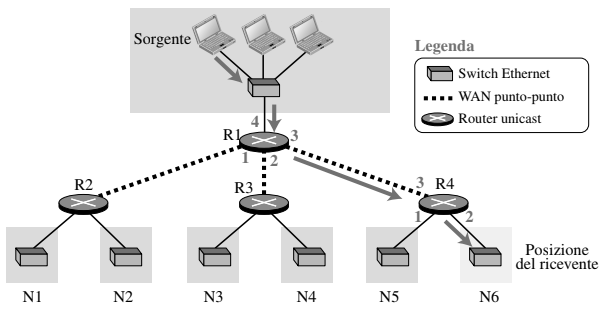
\includegraphics[width=0.7\textwidth]{images/unicast.PNG}
        %\captionof{figure}{Percorso a costo minimo e tabella di inoltro per il nodo $u$}
    \end{minipage}
    
    Il router R1 è responsabile dell' inoltro del datagramma attraverso l'interfaccia 3 e il router R4 deve inoltrare il datagramma attraverso l'interfaccia 2. Quando il datagramma arriva a N6, la consegna all'host di destinazione è di responsabilità della rete. Infatti, il datagramma può essere inviato in broadcast (a tutti gli host della rete) oppure lo switch Ethernet può consegnarlo al solo host di destinazione.
\end{Example}

\subsubsection{Broadcast}
L'invio broadcast implica una comunicazione uno-a-tutti: quando un nodo trasmette un frame, il canale lo diffonde e tutti gli altri nodi ne ricevono una copia. Broadcast può essere eseguito come:
\begin{itemize}
    \item \textit{Uncontrolled flooding:} quando un nodo riceve un pacchetto broadcast, lo duplica e lo invia a tutti i nodi vicini (eccetto a quello da cui lo ha ricevuto). Se il grafo ha cicli, una o più copie del pacchetto cicleranno all’infinito nella rete.
    \item \textit{Controlled flooding:} a sua volta diviso in Sequence number e Reverse path forwarding.

    Con il sequence number non vengono forwardati i pacchetti già ricevuti e inoltrati. Ogni nodo tiene una lista di $(indirizzo IP, \#seq)$ dei pacchetti già ricevuti, duplicati, inoltrati. Quando riceve un pacchetto controlla nella lista, se già inoltrato lo scarta, altrimenti lo forwarda.

    Con il reverse path forwarding (RPF) viene forwardato il pacchetto solo se è arrivato dal link che è sul suo shortest path (unicast) verso la sorgente. RPF elimina il problema di inondare la rete con troppi pacchetti ma non elimina completamente la trasmissione di pacchetti ridondanti. Come soluzione si può costruire lo spanning tree prima di inviare i pacchetti broadcast: si prende un nodo come centro ($E$); ogni nodo invia un messaggio di join in unicast verso il centro; i messaggi vengono inoltrati finchè arrivano a un nodo che già appartiene all’albero o alla radice. I pacchetti vengono inoltrati solo sui link dell’albero, e ogni nodo riceve solo una copia del pacchetto.

    \begin{figure}[ht]
        \centering
        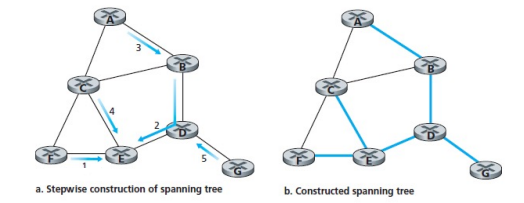
\includegraphics[width=11cm]{images/spanning-tree.PNG}
        \caption{Broadcast sullo spanning tree}
        \label{fig:spanning-tree}
    \end{figure}
\end{itemize}


\subsubsection{Multicast}
Nel multicast è presente una sola sorgente e un gruppo di destinazioni. Il rapporto è uno a molti. In questo tipo di comunicazione, l'indirizzo della sorgente è un indirizzo unicast, mentre l'indirizzo di destinazione è un indirizzo di gruppo, cioè un gruppo di una o più reti di destinazione nelle quali si trova almeno un host che è interessato a ricevere il datagramma multicast. L'indirizzo di gruppo definisce i membri del gruppo stesso.

\begin{Example}{Multicast}{}
    \textit{Nel multicast, un router potrebbe inviare copie multiple dello stesso datagramma attraverso più interfacce di rete.} 

    \begin{minipage}{\textwidth}
        \centering
        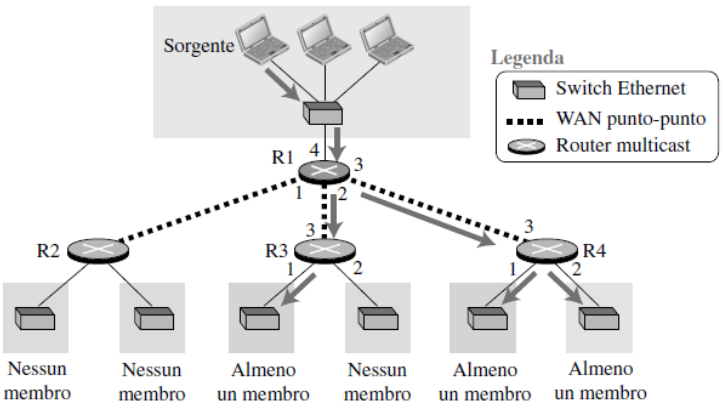
\includegraphics[width=0.7\textwidth]{images/multicast.PNG}
        %\captionof{figure}{Percorso a costo minimo e tabella di inoltro per il nodo $u$}
    \end{minipage}
    
    Nella figura, il router R1 deve inviare il datagramma attraverso le interfacce 2 e 3. Allo stesso modo, il router R4 necessita di inviare il datagramma attraverso tutte le sue interfacce. Il router R3 invece sa che non ci sono membri che appartengono al gruppo multicast nell'area raggiunta dall'interfaccia 2 e quindi invia i datagrammi relativi al gruppo solamente attraverso l'interfaccia 1.
\end{Example}

Occorre distinguere tra multicast e unicast multiplo. La Figura \ref{fig:confronto-multicast} illustra entrambi i concetti.

\begin{figure}[ht]
    \centering
    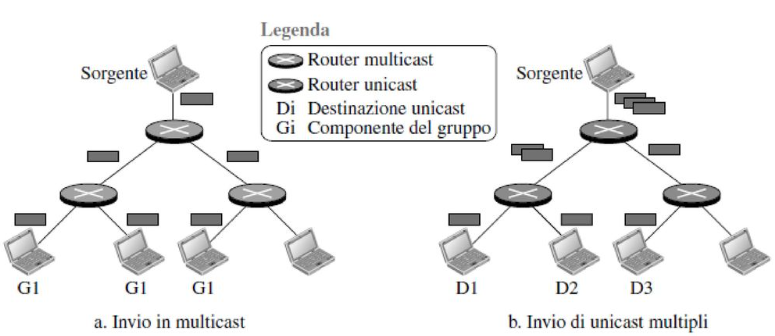
\includegraphics[width=11cm]{images/confronto-multicast.PNG}
    \caption{Confronto tra multicast e unicast multiplo}
    \label{fig:confronto-multicast}
\end{figure}

Il multicast ha inizio con un singolo datagramma spedito dalla sorgente che viene poi duplicato dai router. L'indirizzo di destinazione presente in ogni datagramma è lo stesso per tutti i duplicati. Da notare che tra ogni coppia di router viaggia una singola copia del datagramma.

Nel caso dell'unicast multiplo invece dalla sorgente partono numerosi datagrammi. Ad esempio, se ci sono tre destinazioni, la sorgente invia tre datagrammi distinti, ognuno con un differente indirizzo unicast di destinazione. In questo caso ci possono essere copie multiple del datagramma che viaggiano tra le coppie di router. Ad esempio, se una persona invia un'email a un gruppo di persone quello che avviene è un unicast multiplo. Il software usato per la spedizione della e-mail crea tante copie del messaggio quanti sono i destinatari e le invia una ad una.

\subsubsection{Indirizzi multicast}
Quando inviamo un datagramma unicast a una destinazione, l'indirizzo sorgente del datagramma definisce il mittente e l'indirizzo di destinazione definisce il ricevente. Nella comunicazione multicast, il mittente è solo uno, ma i riceventi sono tanti, a volte migliaia o potenzialmente milioni. Dovrebbe essere chiaro che non possiamo includere gli indirizzi di tutti i destinatari nell'intestazione del datagramma. L'indirizzo di destinazione di un datagramma, come descritto nell'Internet Protocol (IP), deve essere uno solo. Per questa ragione servono degli specifici indirizzi multicast. Un indirizzo multicast definisce un gruppo di destinatari. In altre parole, un indirizzo multicast è l'identificatore di un gruppo. Quando viene formato un nuovo gruppo, composto da vari membri attivi, un'apposita autorità assegnerà un indirizzo multicast inutilizzato a questo nuovo gruppo, indirizzo che servirà per identificare in modo univoco il gruppo. Questo significa che l'indirizzo sorgente di un datagramma in una comunicazione multicast può essere un indirizzo unicast (che individua in modo univoco il mittente), ma l'indirizzo di destinazione può essere un indirizzo multicast (che individua un gruppo). In questo modo, un host che è membro di $n$ gruppi ha in realtà ($n+1$) indirizzi: il suo indirizzo unicast che lo identifica come sorgente o destinazione nelle comunicazioni unicast ed $n$ indirizzi multicast che sono usati solo come indirizzi di destinazione per l'invio di datagrammi a ciascun gruppo.

\begin{figure}[ht]
    \centering
    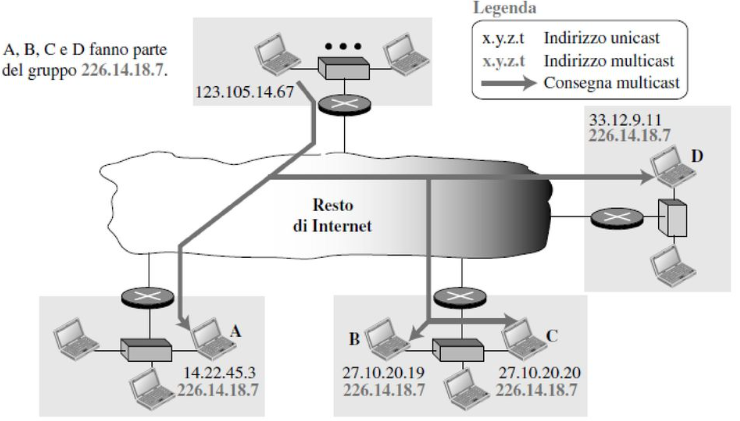
\includegraphics[width=11cm]{images/indirizzi-multicast.PNG}
    \caption{Esempio di utilizzo degli indirizzi multicast}
    \label{fig:indirizzi-multicast}
\end{figure}

Un router o un host di destinazione hanno la necessità di distinguere tra datagrammi unicast e multicast. IPv4 riserva un blocco di indirizzi esclusivamente per il multicast. Nell'indirizzamento con classi tutta la classe D era composta da indirizzi multicast. L'indirizzamento senza classi utilizza lo stesso blocco di indirizzi a cui ora si fa riferimento come \texttt{224.0.0.0/4} (da \texttt{224.0.0.0} a \texttt{239.255.255.255}). 

\begin{figure}[ht]
    \centering
    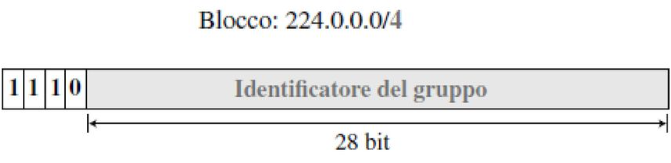
\includegraphics[width=9cm]{images/indirizzi-multicast2.PNG}
    \caption{Un indirizzo multicast in notazione binaria}
    \label{fig:indirizzi-multicast2}
\end{figure}

I primi quattro bit definiscono il blocco, tutti i successivi invece sono a disposizione per identificare gruppi multicast. E' bene notare come il numero di gruppi che possono essere definiti è molto elevato (225).

\subsubsection{Gruppi multicast}
I router non sono a conoscenza dell'appartenenza degli host ai vari gruppi multicast. L'appartenenza ad un gruppo infatti non ha alcuna relazione con il prefisso associato alla rete. L'appartenenza ad un gruppo multicast porta l'host ad avere un indirizzo multicast separato ed aggiuntivo rispetto a quello primario. In secondo luogo, l'appartenenza non è un attributo fisso dell'host; ciascun host può entrare a far parte di nuovi gruppi e lasciarne altri, anche in un periodo di tempo molto breve. Per questa ragione, un router ha bisogno di aiuto per scoprire quali gruppi sono presenti in ciascuna delle sue interfacce. Dopo aver raccolto queste informazioni, il router può propagare l'appartenenza al gruppo ad ogni altro router che faccia uso di un protocollo di routing multicast.

\begin{Example}{Annuncio unicast rispetto ad annuncio multicast}{}
    \begin{minipage}{\textwidth}
        \centering
        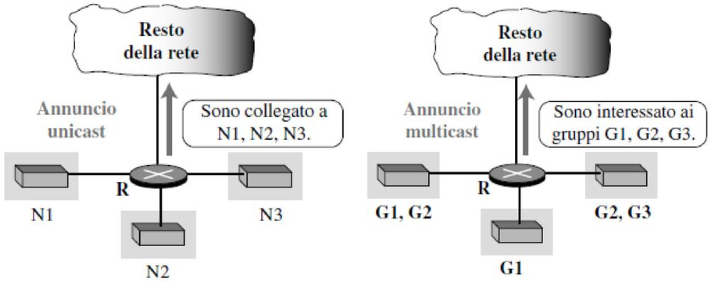
\includegraphics[width=0.7\textwidth]{images/annuncio-multicast.PNG}
        %\captionof{figure}{Percorso a costo minimo e tabella di inoltro per il nodo $u$}
    \end{minipage}

    Nel caso dell'unicast, il router R sa che gli host con i prefissi N1, N2 e N3 sono connessi alle sue interfacce; esso propaga quindi queste informazioni al resto della rete. Nel caso del multicast, il router R necessita di conoscere se ciascun host fa parte di qualche gruppo multicast (G1, G2 o G3).
\end{Example}

In altre parole, nel routing unicast è sufficiente avere un protocollo d'instradamento per diffondere le informazioni relative ai vari collegamenti. Invece, nel caso del multicast occorrono due protocolli: il primo per raccogliere le informazioni di appartenenza ai gruppi e il secondo per diffonderle.

\subsubsection{Internet Group Management Protocol (IGMP)}
Il protocollo che oggi viene usato per raccogliere informazioni relative all'appartenenza a gruppi è l'Internet Group Management Protocol (IGMP). L'IGMP è un protocollo di livello rete e così come l'ICMP si tratta anche in questo caso di un protocollo ausiliario, che viene considerato parte integrante di IP. Lavora tra un host e il router che gli è direttamente connesso e offre agli host il mezzo di informare i router ad essi connessi del fatto che un’applicazione in esecuzione vuole aderire ad uno specifico gruppo multicast. I messaggi IGMP, così come quelli ICMP, vengono incapsulati in datagrammi IP.
\begin{itemize}
    \item \texttt{Membershp query}. Periodicamente tutti gli host collegati ad un router vengono contattati per mezzo di un messaggio query. Il messaggio chiede a ciascun host di indicare il suo stato di appartenenza a gruppi multicast.

    \item \texttt{Membershp report}. Viene inviato da un host al suo router, come risposta ad un messaggio query, per informare il router su un’adesione, anche non inseguito a una query (al momento dell’adesione). Il messaggio contiene una lista di record, in ciascun record l'host fornisce l'identificatore di un gruppo (il suo indirizzo multicast) e la lista di tutte le fonti da cui l'host è interessato a ricevere messaggi di gruppo (versione inclusiva) oppure la lista delle fonti da cui non è interessato a ricevere messaggi di gruppo (versione esclusiva).

    \item \texttt{Leave group}. Viene inviato da host al suo router quando si lascia un gruppo. Il leave group è opzionale: il router può capire che non ci sono più host associati a un gruppo quando non riceve report in risposta a query.
\end{itemize}

\begin{figure}[ht]
    \centering
    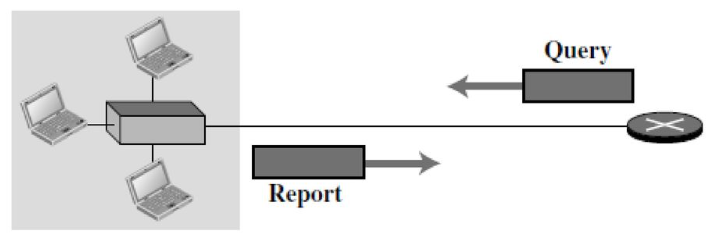
\includegraphics[width=8cm]{images/igmp.PNG}
    \caption{Funzionamento di IGMP}
    \label{fig:igmp}
\end{figure}

Se un host desidera entrare a far parte di gruppo aspetterà fino a quando non riceve un messaggio query per poi inviare la sua richiesta nel messaggio report di risposta. Se invece un host intende lasciare il gruppo, esso semplicemente non risponde al messaggio query. Nel caso nessun altro host risponda al messaggio corrispondente, il gruppo verrà eliminato dal database del router. 

Un router multicast tiene una lista per ciascuna sottorete dei gruppi multicast con un timer per membership. La membership deve essere aggiornata da report inviati prima della scadenza del timer, può essere anche aggiornata tramite messaggi di leave espliciti.

\subsubsection{Instradamento multicast}
Nell'instradamento multicast, come così come in quello unicast, occorre creare tabelle di routing per instradare in modo ottimale i pacchetti dalla sorgente alla loro destinazione. Tuttavia, come abbiamo detto in precedenza, le decisioni sull'instradamento multicast di ciascun router dipendono non solo dalla destinazione del pacchetto ma anche dalla sorgente del pacchetto stesso. Il coinvolgimento della sorgente nel processo di instradamento rende il routing multicast molto più complesso rispetto a quello unicast. Fra la popolazione complessiva di router solo alcuni (quelli collegati a
host del gruppo multicast) dovranno ricevere traffico multicast. E' necessario un protocollo che coordini i router multicast in Internet (instradare pacchetti multicast dalla sorgente alla destinazione). A grandi linee sono stati sviluppati due differenti approcci per l'instradamento multicast: quello definito Source-based Tree e quello chiamato Group-shared Tree.

\begin{itemize}
    \item \textit{Approccio Source-based Tree.} Nell'approccio Source-based Tree ciascun router crea un albero diverso per ogni combinazione di sorgente e gruppo. In altre parole, se in una rete ci sono $m$ gruppi ed $n$ sorgenti, un router necessita di creare ($m \times n$) alberi d'instradamento. In ciascun albero, la sorgente è la radice, i membri del gruppo sono le foglie e il router stesso si trova da qualche parte nell'albero.

    \item \textit{Approccio Group-shared Tree.} Nell'approccio Group-shared Tree si designa un router che finge di essere la sorgente di ciascun gruppo. Il router designato, che viene chiamato core o rendezvous-point router, agisce come rappresentante del gruppo. Qualsiasi sorgente che abbia un pacchetto da inviare a un membro di questo gruppo, lo invia al core router (usando unicast) e il core router è poi responsabile del multicast per gli altri componenti del gruppo. Il core router crea un singolo albero d'instradamento con se stesso come radice e gli altri router come foglie (purché abbiano host attivi come componenti del gruppo). In questo approccio, ci sono $m$ core router (uno per ogni gruppo) e ogni core router costruisce un albero d'instradamento, per un totale di $m$ alberi. Questo significa che il numero degli alberi d'instradamento viene ridotto da ($m\times n$) dell'approccio Source-based Tree a $m$.
\end{itemize}

\section{IPv6}
L'esaurimento degli indirizzi e alcune limitazioni di IPv4, già nei primi anni '90, hanno portato allo sviluppo di una nuova versione del protocollo. Questa nuova versione, chiamata Internet Protocol versione 6 (IPv6) o IP di nuova generazione (IP new generation, IPng) è nata con lo scopo di aumentare lo spazio degli indirizzi rispetto a IPv4, ridisegnare il formato dei datagrammi IP e allo stesso tempo rivedere anche alcuni protocolli ausiliari come ICMP. Quanto segue mostra i principali cambiamenti nel protocollo IPv6.
\begin{itemize}
    \item \textit{Spazio degli indirizzi di dimensione maggiore.} Un indirizzo IPv6 è lungo 128 bit. Paragonato ai 32 bit dell'IPv4, è un enorme aumento (2\% volte) dello spazio degli indirizzi.
    \item \textit{Miglior formato dell'intestazione.} IPv6 utilizza un nuovo formato per l'intestazione (header) dei datagrammi. Nell'intestazione IPv6 le opzioni sono separate dall'intestazione di base e inserite, quando necessario, tra l'intestazione di base e i dati. Ciò semplifica e velocizza il processo di routing visto che la maggior parte delle opzioni non è necessario che sia controllata dai router.
    \item \textit{Nuove opzioni.} IPv6 supporta nuove opzioni per consentire l'implementazione di funzionalità aggiuntive.
    \item \textit{Possibilità di estensione.} L'IPv6 è progettato per consentire l'estensione del protocollo se richiesto dall'introduzione di nuove tecnologie o applicazioni.
    \item \textit{Supporto per l'allocazione delle risorse.} In IPv6 è stato rimosso il campo tipo del servizio (Type Of Service, TOS) che è presente in IPv4. Al suo posto sono stati aggiunti due nuovi campi, classe di traffico ed etichetta di flusso, per consentire alla sorgente di richiedere un trattamento speciale per il datagramma. Il meccanismo, se fosse supportato dai router, potrebbe migliorare la gestione del traffico audio o video in tempo reale.
    \item \textit{Maggiore sicurezza.} Le opzioni relative a crittografia ed autenticazione permettono di migliorare la riservatezza e verificare l'integrità dei datagrammi.
\end{itemize}

L'adozione di IPv6 è stata lenta. Il motivo principale che ha portato al suo sviluppo, cioè il progressivo esaurimento degli indirizzi IPv4, è stato rallentato grazie a tre rimedi a breve termine: l'indirizzamento senza classi, l'uso del protocollo DHCP e soprattutto la diffusione del NAT. Il fatto che si tratti di soluzioni a breve termine, che non risolvono a fondo il problema, e l'uso sempre più ampio di nuovi servizi (per esempio, l'uso del protocollo IP in mobilità, la telefonia basata su IP ecc.) prima o poi richiederanno la sostituzione totale di IPv4 con IPv6. In passato si prevedeva che questa migrazione sarebbe avvenuta entro il 2010, cosa che in effetti non è successa. Le previsioni attuali parlano invece del 2020, ma probabilmente si andrà ben oltre.

\subsection{Formato dei datagrammi IPv6}
Ciascun datagramma è composto da un'intestazione di base (base header) seguita dai dati (payload). L'intestazione di base occupa 40 byte, mentre il payload può arrivare fino a 65.535 byte.

\begin{figure}[ht]
    \centering
    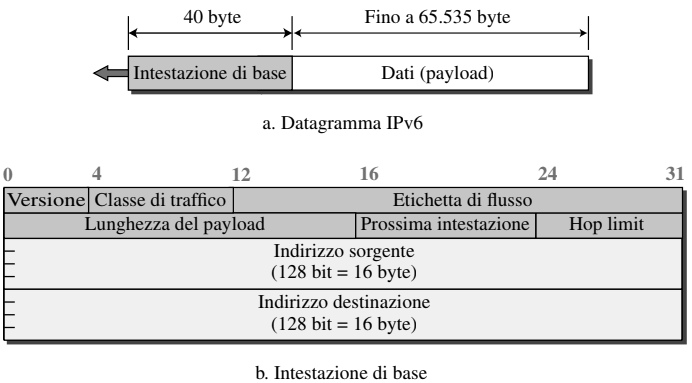
\includegraphics[width=11cm]{images/formato-ipv6.PNG}
    \caption{Formato dei datagrammi IPv6}
    \label{fig:formato-ipv6}
\end{figure}

\begin{itemize}
    \item \textit{Versione (version).} Il campo versione (4 bit) definisce il numero di versione del protocollo IP. Per l'IPv6, il valore è 6.
    \item \textit{Classe di traffico (traffic class).} Il campo classe di traffico (8 bit) è utilizzato per distinguere il tipo di servizio di trasferimento a seconda della tipologia di dati contenuti nel payload. Esso sostituisce il campo tipo di servizio (Type Of Service, TOS) che è presente in IPv4.
    \item \textit{Etichetta di flusso (flow label).} L'etichetta di flusso (20 bit) dovrebbe permettere una nuova gestione dei dati sotto forma di flusso di datagrammi, rispetto ai singoli datagrammi indipendenti come accade in IPv4.
    \item \textit{Lunghezza del payload (payload length).} Il campo lunghezza del payload (2 byte) definisce la lunghezza del datagramma IP escludendo l'intestazione. Si noti che in IPv4 ci sono due campi legati dalla lunghezza: lunghezza dell'intestazione e lunghezza totale. Invece in IPv6, la lunghezza dell'intestazione di base è fissa (40 byte), quindi è necessario indicare solamente la lunghezza del payload.
    \item \textit{Prossima intestazione (next header).} La prossima intestazione è un campo (8 bit) che definisce il tipo della prima intestazione estesa (extension header), se presente, o il tipo dei dati che seguono l'intestazione di base all'interno del payload. Questo campo è simile al campo "protocollo" che è presente in IPv4.
    \item \textit{Hop limit (numero massimo di salti).} Il campo hop limit ha la stessa funzione del campo TTL in IPv4.
    \item \textit{Indirizzo sorgente e indirizzo destinazione (source and destination address).} I campi indirizzo sorgente e destinazione sono indirizzi Internet da 16 byte (128 bit) che identificano la sorgente originale del datagramma e la sua destinazione.
    \item \textit{Dati (payload).} Se confrontato con IPv4, il campo payload in IPv6 ha una forma e un significato differenti. Il campo dati in IPv6 può contenere una combinazione di zero o più intestazioni estese (usate per rappresentare le varie opzioni) seguite dai dati provenienti da altri protocolli (UDP, TCP e così via). In IPv6, le opzioni, che fanno parte dell'intestazione in IPv4, sono implementate sotto forma di intestazioni estese. Il campo dati può contenere tante intestazioni quante ne sono necessarie. Ogni intestazione è formata da due campi obbligatori, intestazione successiva (next header) e lunghezza (length), seguite dalle informazioni specifiche della varie opzioni. Si noti l'uso che viene fatto del campo "prossima intestazione" (next header); definisce il tipo della prossima intestazione quando si riferisce a un'opzione oppure identifica il protocollo incapsulato nel payload del datagramma.
\end{itemize}

\subsection{Passaggio da IPv4 a IPv6}
Anche se è pronta una nuova versione del protocollo IP, rimane da capire come può essere fatto il passaggio dalla versione corrente a quella nuova. La prima soluzione che viene in mente, la più banale, è definire un giorno di passaggio nel quale tutti gli host e router smetteranno di usare IPv4 ed inizieranno ad usare solo IPv6. Ovviamente la transizione non può essere fatta in questo modo. A causa dell'enorme numero di sistemi in rete la migrazione non può avvenire improvvisamente. Ci sarà bisogno di una quantità di tempo considerevole prima che tutti i sistemi siano aggiornati. La transizione dovrà essere studiata accuratamente per evitare problemi tra il vecchio sistema e quello nuovo. L'IETF ha studiato tre strategie che possono essere implementate in questa fase: il dual stack (doppia pila di protocolli), il tunneling e la traduzione dell'intestazione (header translation).

\subsubsection{Dual stack}
La strategia prevede che tutti gli host, durante la transizione, abbiano una doppia pila di protocolli per la comunicazione in rete. In altre parole, ciascun host (o router) deve eseguire IPv4 e IPv6 simultaneamente fino a quando tutta la rete non sarà passata ad IPv6.

\begin{figure}[ht]
    \centering
    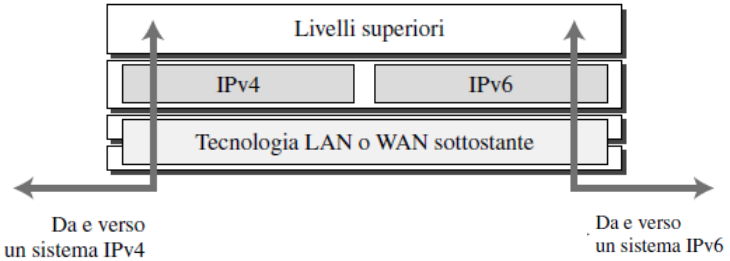
\includegraphics[width=10cm]{images/dual-stack.PNG}
    \caption{Dual stack}
    \label{fig:dual-stack}
\end{figure}

Per determinare quale versione utilizzare quando si invia un pacchetto a una destinazione, l'host sorgente interroga il DNS. Se il DNS restituisce un indirizzo IPv4 allora l'host invía un pacchetto IPv4. Se il DNS restituisce un indirizzo IPv6 allora l'host invia un pacchetto IPv6.

\subsubsection{Tunneling}
Il tunneling è una tecnica utilizzata quando due host che usano IPv6 vogliono comunicare tra loro ma i datagrammi devono attraversare una regione della rete che usa solo IPv4. Per passare attraverso questa regione i datagrammi devono necessariamente avere un indirizzo IPv4. La soluzione è quella di incapsulare ciascun datagramma IPv6 nel payload di un datagramma IPv4. Una volta superata la tratta IPv4, il datagramma IPv6 potrà essere nuovamente estratto. E' come se i datagrammi IPv6 viaggiassero all'interno di un tunnel tra due isole IPv6. Per rendere esplicito il fatto che il datagramma IPv4 sta trasportando un datagramma IPv6, il valore del protocollo nell'intestazione del datagramma IPv4 viene impostato a 41.

\begin{figure}[ht]
    \centering
    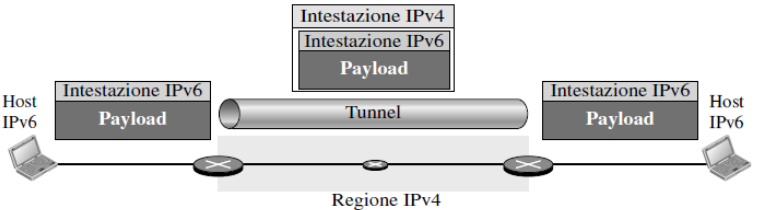
\includegraphics[width=11cm]{images/tunneling.PNG}
    \caption{Strategia di tunneling}
    \label{fig:tunneling}
\end{figure}

\subsubsection{Traduzione dell'intestazione}
La traduzione dell'intestazione (header translation) sarà necessaria quando la maggior parte di Internet sarà migrata ad IPv6, con alcuni sistemi residui ancora basati su IPv4. Supponiamo che il mittente intenda (o debba) usare IPv6, ma che il ricevente non sia in grado di supportarlo. In questo caso il meccanismo di tunneling non funziona. L'unica alternativa è quella di effettuare una traduzione completa dell'intestazione del datagramma, in modo di convertirla da IPv6 a IPv4, prima che il datagramma arrivi a destinazione.

\begin{figure}[ht]
    \centering
    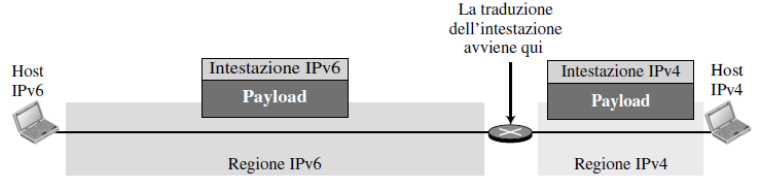
\includegraphics[width=11cm]{images/traduzione-intestazione.PNG}
    \caption{Strategia di traduzione dell'intestazione}
    \label{fig:traduzione-intestazione}
\end{figure}